\documentclass[class=report,crop=false]{standalone}
\usepackage[screen]{../exo7book}

% Commande ponctuelle
\newcommand{\alenvers}[1]{\rotatebox[origin=c]{180}{#1}}
\newcommand{\vect}{\overrightarrow}


\begin{document}

%====================================================================
\chapitre{Calcul formel}
%====================================================================



%\insertvideo{4DY7CI_Q1zM}{partie 1. Premiers pas avec Sage}
%
%\insertvideo{nT94JZKl3cg}{partie 2. Structures de contrôle avec \Sage}
%
%\insertvideo{2lmDmNL8DwI}{partie 3. Suites récurrentes et preuves formelles}
%
%\insertvideo{ciw-QPp7p98}{partie 4. Suites récurrentes et visualisation}
%
%\insertvideo{s0aR-QbmTAo}{partie 5. Algèbre linéaire}

\insertvideo{kvviYsb9Ltk}{partie 6a. Courbes et surfaces}

\insertvideo{ttiZ7bDXeEA}{partie 6b. Courbes et surfaces}

\insertvideo{teKCZNGXGkQ}{partie 7. Calculs d'intégrales}
%
%\insertvideo{ybVCQQtHIDk}{partie 8. Polynômes}
%
%\insertvideo{lSn_KZvTCOs}{partie 9. \'Equations différentielles}

\setcounter{section}{5}


%%%%%%%%%%%%%%%%%%%%%%%%%%%%%%%%%%%%%%%%%%%%%%%%%%%%%%%%%%%%%%%%%
%\section{Premiers pas avec \Sage}
%
%Le calcul formel est un domaine charnière entre mathématiques et informatique. 
%L'objectif de ce cours est d'obtenir des algorithmes efficaces afin de manipuler des 
%objets mathématiques abstraits tels que les fonctions, 
%les polynômes, les matrices, etc. 
%\`A notre niveau, le calcul formel ou symbolique sera synonyme de <<mathématiques effectives et efficaces>>.
%
%
%%--------------------------------------------------------
%\subsection{Hello world!}
%
%Servons-nous d'abord de \Sage\ comme d'une calculatrice :
%\begin{tp}
%\sauteligne
%\begin{enumerate}
%  \item Calculer $1+2 \times 3^4$.
%  \item Calculer $\frac{22}{33}$.
%  \item Calculer $\cos(\frac{\pi}{6})$.
%\end{enumerate}  
%\end{tp}
%
%Voilà les résultats : 
%\insertcode{algos/hello-world-tex.sage}{hello-world.sage}
%
%
%On retient que :
%\begin{itemize}
%  \item \Sage\ connaît les opérations classiques $+$, $-$, $\times$, $/$.
%  La puissance $a^b$ s'écrit
%  \codeinline{a^b} ou \codeinline{a**b}.
%  
%  \item \Sage\ fait des calculs exacts, il simplifie $\frac{22}{33}$ en 
%  $\frac{2}{3}$, contrairement à une banale calculatrice qui afficherait $0.6666\ldots$
%  
%  \item \Sage\  manipule les fonctions et les constantes usuelles : 
%  par exemple $\cos\left(\frac{\pi}{6}\right) = \frac{\sqrt{3}}{2}$.
%\end{itemize}
%
%Dans toute la suite, on omettra l'invite de commande << \codeinline{sage:} >>.
%En fin de section vous trouverez davantage d'informations sur la mise en place de \Sage.
%
%%--------------------------------------------------------
%\subsection{Calcul formel}
%
%L'utilisation d'un système de calcul symbolique conduit le mathématicien 
%à un type de démarche auquel il n'est  traditionnellement pas habitué : 
%l'expérimentation !
%\begin{enumerate}
%  \item Je me pose des questions.
%  
%  \item J'écris un algorithme pour tenter d'y répondre.
%  
%  \item Je trouve une conjecture sur la base des résultats expérimentaux.
%  
%  \item Je prouve la conjecture.
%\end{enumerate}
%
%\begin{tp}
%\sauteligne
%\begin{enumerate}
%  \item Que vaut le nombre complexe $(1-\ii)^k$, pour $k\ge 0$ ?
%  \item Les nombres de la forme $F_n = 2^{(2^n)}+1$ sont-ils tous premiers ?
%\end{enumerate}  
%\end{tp}
%
%
%Nous pouvons faire des calculs avec les nombres complexes.
%En posant $z= 1 - \ii$, on calcule successivement la partie réelle (par la commande 
%\codeinline{real_part}), la partie imaginaire (\codeinline{imag_part}), le module 
%(\codeinline{abs}) et l'argument (\codeinline{arg}) de $z^0, z^1, z^2,\ldots$.
%
%\insertcode{algos/motiv-calcul-formel-tex1.sage}{motiv-calcul-formel.sage (1)}
%
%\begin{tabular}{llll}
%\begin{lstlisting}
%0 1
%1 -I + 1
%2 -2*I
%3 -2*I - 2
%4 -4
%\end{lstlisting}
%&
%\begin{lstlisting}
%5 4*I - 4
%6 8*I
%7 8*I + 8
%8 16
%9 -16*I + 16
%\end{lstlisting}
%&
%\begin{lstlisting}
%10 -32*I
%11 -32*I - 32
%12 -64
%13 64*I - 64
%14 128*I
%\end{lstlisting}
%&
%\begin{tabular}{l}
%\pause 
%\!\!\!\!$z^{4\ell}=(-1)^\ell 2^{2\ell}$\\
%\!\!\!\!$z^{4\ell+1}=(-1)^\ell 2^{2\ell}(1-\ii)$\\
%\!\!\!\!$z^{4\ell+2}=(-1)^\ell 2^{2\ell}(-\ii)$\\
%\!\!\!\!$z^{4\ell+3}=(-1)^\ell 2^{2\ell}(-1-\ii)$\\
%\end{tabular}
%\end{tabular}
%
%On remarque expérimentalement une structure assez simple. 
%Par exemple pour passer de $z_k = (1+\ii)^k$ à $z_{k+1} = (1+\ii)^{k+1}$ 
%le module est multiplié par $\sqrt 2$ alors que 
%l'argument change de $-\frac{\pi}{4}$. On en conjecture $z_{k+1} = \sqrt{2} e^{-\frac{\ii\pi}{4}} z_k$.
%Comme $z_0 = (1-\ii)^0 = 1$ alors on conjecture $z_k = \sqrt{2}^k e^{-\frac{k\ii\pi}{4}}$.
%
%Passons à la preuve : en écrivant sous la forme module-argument $z = \sqrt{2} e^{-\frac{\ii\pi}{4}}$,
%on obtient bien que $z^k = \sqrt{2}^k e^{-\frac{k\ii\pi}{4}}$.
%On pourrait aussi obtenir une expression simple en discutant selon les valeurs de $k$ modulo $8$. 
%
%\bigskip
%
%Le calcul formel permet aussi d'éviter de passer des années à essayer de montrer un résultat qui s'avère faux
%au final. Pierre de Fermat pensait que tous les nombres de la forme $F_n = 2^{2^n}+1$ étaient premiers.
%Cent ans plus tard, Euler calcule que $F_5 = 4\;294\;967\;297 = 641 \times 6\;700\;417$ n'est pas un nombre premier.
%
%\insertcode{algos/motiv-calcul-formel-tex2.sage}{motiv-calcul-formel.sage (2)}
%
%%--------------------------------------------------------
%\subsection{Calcul formel vs calcul numérique}
%
%Même si \Sage\ est conçu pour le calcul symbolique, il sait aussi 
%effectuer des calculs numériques. Bien que non exact, le calcul numérique possède plusieurs avantages :
%il est plus rapide, souvent suffisant pour les applications pratiques et peut aussi être plus lisible.
%
%\begin{tp}
%Quelle est la limite de la suite définie par récurrence :
%$$u_0 = 1 \qquad u_{n+1} = \sqrt{1+u_n} \ \text{ pour } n \ge 0 \quad \text{ ?}$$
%\end{tp}
%
%Si on calcule formellement les premiers termes on trouve :
%$$u_0=1 \qquad u_1 = \sqrt{2} \qquad u_2 = \sqrt{1+\sqrt{2}} \qquad
%u_3 = \sqrt{1+\sqrt{1+\sqrt{2}}} \qquad u_4 = \sqrt{1+\sqrt{1+\sqrt{1+\sqrt{2}}}}$$
%Ce qui n'éclaire pas vraiment sur le comportement de la suite.
%
%\insertcode{algos/calcul-numerique.sage}{calcul-numerique.sage}
%
%Par contre au vu des approximations :
%$$\begin{array}{rcl}
%u_0 &=& 1 \\
%u_1 &=& 1.4142\ldots \\
%u_2 &=& 1.5537\ldots\\
%u_3 &=& 1.5980\ldots\\
%u_4 &=& 1.6118\ldots\\
%u_5 &=& 1.6161\ldots\\
%\end{array}$$
%on peut émettre plusieurs conjectures : la suite est croissante, elle est majorée par $2$
%et converge. En poussant les calculs, une approximation de la limite est
%$1.618033\ldots$
%Les plus observateurs auront reconnu une approximation 
%du nombre d'or $\phi = \frac{1+\sqrt{5}}{2}$, solution positive 
%de l'équation $x^2-x-1$. On renvoie à un cours d'analyse pour la preuve
%que la suite $(u_n)$ converge effectivement vers $\phi$.
%
%%--------------------------------------------------------
%\subsection{Graphiques}
%
%La production de graphiques est un formidable outil qui permet de mettre en lumière des phénomènes complexes.
%
%\begin{tp}
%Soit la fonction $f(x)= \sin(x) \cdot \exp(x)$.
%Calculer les premiers polynômes de Taylor associés aux développements limités de $f$ en $0$. 
%Tracer leurs graphes. Quelles propriétés des développements limités cela met-il en évidence ?
%\end{tp}
%
%\begin{center}
%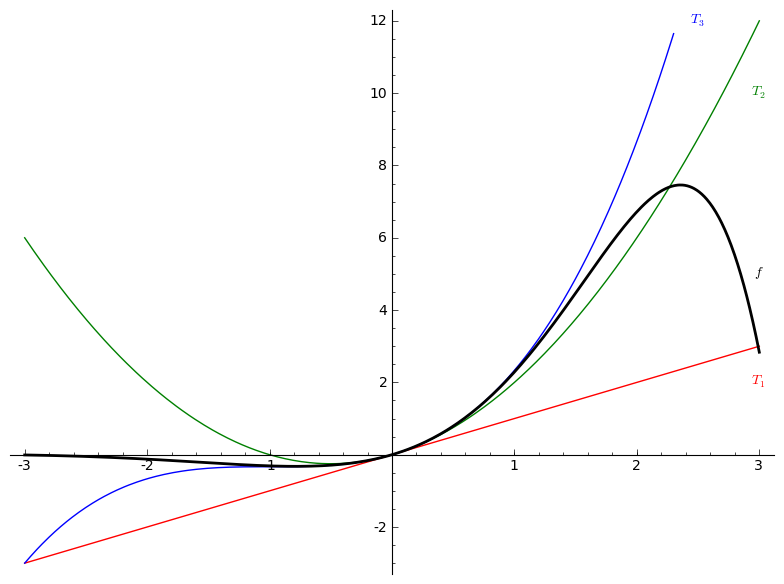
\includegraphics[scale=0.5]{figures/formel-taylor}
%\end{center}
%
%
%\begin{itemize}
%  \item Après avoir défini la fonction $f$ par \codeinline{f = sin(x)*exp(x)}, la commande 
%  \codeinline{taylor(f,x,0,n)} renvoie le DL de
%  $f$ en $x=0$ à l'ordre $n$, par exemple ici 
%  $f(x) = x + x^2 + \frac13 x^3+ \epsilon(x) x^3$, donc  $T_1(x) = x$,
%  $T_2(x)=x+x^2$, $T_3(x) =  x + x^2 + \frac13 x^3$.
%  
%  \item La commande \codeinline{plot(f,(a,b))} trace le graphe de $f$ sur l'intervalle $[a,b]$.
%\end{itemize}
%
%
%Il est perceptible que :
%\begin{itemize}
%  \item Les polynômes de Taylor sont une bonne approximation de la fonction au voisinage d'un point.
%  \item Plus l'ordre du DL est élevé, meilleure est l'approximation.
%  \item L'approximation est seulement \emph{locale} : loin du point considéré (ici l'origine)
%  les polynômes de Taylor n'approchent plus du tout la fonction.
%\end{itemize}
%
%\bigskip
%
%Il est possible de tracer une grande variété de graphiques.
%Voici par exemple la courbe de Lissajous d'équation $t \mapsto \big(\cos(3t),\sin(4t)\big)$
%et le graphe de la fonction de deux variables définie par 
%$f(x,y)= \cos(xy)$.
%Les commandes sont :
%\begin{itemize}
%  \item \codeinline{parametric_plot((cos(3*t),sin(4*t)),(t,0,2*pi))}
%  \item \codeinline{plot3d(cos(x*y),(x,-4,4),(y,-4,4))}
%\end{itemize}
%
%Attention ! Il faut avoir au préalable définir les variables utilisées : \codeinline{var('t')}
%et \codeinline{var('x,y')}. (En fait, seule la variable $x$ est définie par défaut dans \Sage.)
%
%\begin{center}
%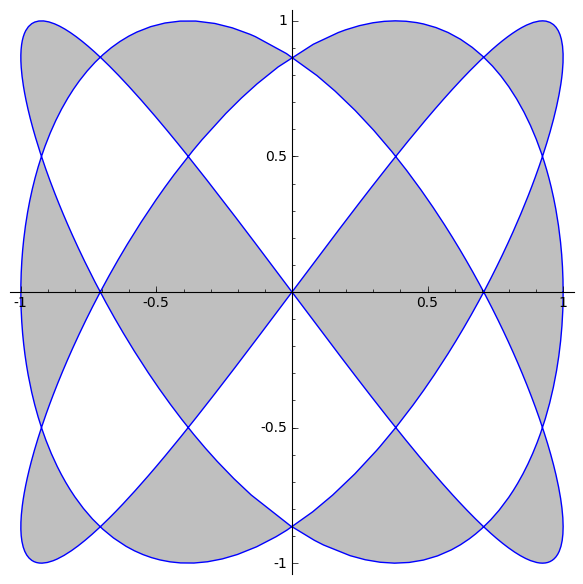
\includegraphics[scale=0.3]{figures/formel-lissajou}
%\includegraphics[scale=0.25]{figures/formel-surface}
%\end{center}
%
%%--------------------------------------------------------
%\subsection{Le calcul formel peut-il tout faire ?}
%
%Le calcul formel ne résout malheureusement pas tous les problèmes 
%de mathématique d'un coup de baguette magique !
%
%
%\begin{tp}
%\sauteligne
%\begin{enumerate}
%  \item Pouvez-vous calculer les solutions réelles de $x^k-x-1=0$ pour les entiers $k \ge 2$ ?
%  \item Est-ce que \Sage\ sait que toutes ces expressions sont nulles ?
%  $$2^{10} - 1024 \qquad (x+1)^2-x^2-2x-1 \qquad \sin^2(x)+\cos^2(x) - 1$$
%\end{enumerate}  
%\end{tp}
%
%
%\begin{enumerate}
%  \item La première limitation est propre aux mathématiques : on ne peut pas trouver 
%une écriture explicite des solutions de toutes les équations.
%Pour $x^2-x-1=0$ à l'aide de la commande
%\codeinline{solve(x^2-x-1==0,x)} on trouve bien les deux solutions
%$\frac{1+\sqrt5}{2}$ et $\frac{1-\sqrt5}{2}$.
%Par contre \codeinline{solve(x^5-x-1==0,x)} ne renvoie pas les solutions, 
%mais il renvoie l'équation qui définit les solutions (ce qui ne nous avance guère).
%Ce n'est pas ici un problème de \Sage.
%En effet, il n'est mathématiquement pas possible d'exprimer la solution réelle de $x^5-x-1=0$ 
%à l'aide de racines ($\sqrt{\phantom{0}}, \sqrt{\phantom{0}}, 
%\sqrt[3]{\phantom{0}}, \sqrt[4]{\phantom{0}},\ldots$). 
%C'est seulement possible jusqu'au degré $4$.
%Par contre on obtient une approximation de la solution réelle par la commande 
%\codeinline{find_root(x^5-x-1==0,-1,2)} en précisant que l'on 
%cherche la solution sur l'intervalle $[-1,2]$.
%  
%  \item 
%  \begin{enumerate}
%    \item Sans problème \codeinline{2^10-1024} renvoie $0$.
%    \item Il est nécessaire de développer pour trouver $0$ : \codeinline{expand((x+1)^2-x^2-2*x-1)}.
%    \item Il faut explicitement préciser de simplifier l'expression trigonométrique :
%    d'abord \codeinline{f = sin(x)^2+cos(x)^2 - 1} puis on demande de simplifier \codeinline{f.simplify_trig()}
%    pour obtenir $0$.  
%  \end{enumerate}
%\end{enumerate}
%
%\bigskip
%
%  Il n'est pas du tout évident pour un ordinateur de reconnaître les identités comme $(a+b)^2 = a^2+2ab+b^2$
%  ou bien $\cos^2(x)+\sin^2(x)=1$. Souvenez-vous d'ailleurs qu'il faut plusieurs années d'apprentissage 
%  pour les assimiler. Lorsqu'il y a plusieurs écritures d'une même expression, 
%  il n'est pas non plus évident pour l'ordinateur de savoir quelle forme est la plus adaptée à l'utilisateur.
%  Par exemple, selon le contexte, les trois écritures sont utiles : $(a-b)^3 = (a-b)(a^2-2ab+b^2)= a^3-3a^2b+3a^2b-b^3$.
%  Il faudra donc <<guider>> le logiciel de calcul formel avec les fonctions 
%  \codeinline{expand}, \codeinline{factor}, \codeinline{simplify}...
%
%\begin{remarque*}
%Pour avoir une idée de la difficulté à identifier deux expressions, voici 
%une représentation de la façon dont les expressions $(a+b)^2$ et $a^2+2ab+b^2$ sont stockées 
%dans le logiciel.
%
%\begin{center}
%\begin{tikzpicture}
%
%\node (A1) at (0,0) {\texttt{a}};
%\node (A2) at (1,0) {\texttt{b}};
%\node (B1) at (0.5,1) {\texttt{+}};
%\node (B2) at (1.5,1) {\texttt{2}};
%\node (C) at (1,2) {\texttt{\^}};
%
%\draw (A1.north) -- (B1.south west);
%\draw (A2.north) -- (B1.south east);
%\draw (B1.north) -- (C.south west);
%\draw (B2.north) -- (C.south east);
%
%\node at (1,-1) {$(a+b)^2$};
%
%
%\begin{scope}[xshift=5cm]
%\node (AA1) at (0,0) {\texttt{a}};
%\node (AA2) at (1,0) {\texttt{2}};
%\node (AA3) at (2,0) {\texttt{2}};
%\node (AA4) at (3,0) {\texttt{a}};
%\node (AA5) at (4,0) {\texttt{b}};
%\node (AA6) at (5,0) {\texttt{b}};
%\node (AA7) at (6,0) {\texttt{2}};
%\node (BB1) at (0.5,1) {\texttt{\^}};
%\node (BB2) at (3,1) {\texttt{*}};
%\node (BB3) at (5.5,1) {\texttt{\^}};
%\node (CC) at (3,2) {\texttt{+}};
%
%\draw (AA1.north) -- (BB1.south west);
%\draw (AA2.north) -- (BB1.south east);
%\draw (AA3.north) -- (BB2.south west);
%\draw (AA4.north) -- (BB2.south);
%\draw (AA5.north) -- (BB2.south east);
%\draw (AA6.north) -- (BB3.south west);
%\draw (AA7.north) -- (BB3.south east);
%
%\draw (BB1.north) -- (CC.south west);
%\draw (BB2.north) -- (CC.south);
%\draw (BB3.north) -- (CC.south east);
%
%\node at (3,-1) {$a^2+2ab+b^2$};
%\end{scope}
%
%\end{tikzpicture}
%\end{center}
%\end{remarque*}
% 
%  
%%--------------------------------------------------------
%\subsection{Un peu plus sur \Sage}
%
%
%
%
%Ce cours n'a pas pour but d'être un manuel d'utilisation du logiciel \Sage.
%Vous trouverez sur internet des tutoriels pour démarrer et pour un usage avancé : \\
%\centerline{\href{http://www.sagemath.org/fr/}{Site officiel de \Sage}}
%Il existe aussi un livre gratuit : \\
%\centerline{\href{http://sagebook.gforge.inria.fr/}{Calcul mathématique avec \Sage}}
%
%Une façon simple d'obtenir de l'aide pour une commande \Sage\ 
%est d'utiliser le point d'interrogation : \codeinline{ln?} (ou bien \codeinline{help(ln)}).
%Vous y apprendrez que la fonction \codeinline{ln} est le logarithme naturel.
%
%
%\bigskip
%Il y a deux façons d'utiliser \Sage\ :
%\begin{itemize}
%  \item \emph{En ligne de commande} : vous obtenez une fenêtre avec l'invite
%  \codeinline{sage} : puis vous tapez vos commandes (en n'oubliant pas de faire une copie de
%  votre travail dans un fichier texte du type \codeinline{mon_programme.sage}).
%  
%  \item \emph{Dans votre navigateur} : à partir de l'invite \codeinline{sage:}
%  vous tapez \codeinline{notebook()} pour obtenir une interface complète et conviviale.
%\end{itemize}
%
%Voici une liste de fonctions usuelles :
%\begin{center}
%\setlength{\arrayrulewidth}{0.05mm}
%%\begin{tabular}{|l|l|l|} \hline
%\begin{tabular}[t]{|c|c@{\vrule depth 1.2ex height 3ex width 0mm \ }|} 
%\hline
%   \codeinline{abs(x)}     &   $|x|$      \\ \hline
%   \codeinline{x^n} \  ou \  \codeinline{x**n}     &   $x^n$      \\ \hline
%   \codeinline{sqrt(x)}    &  $\sqrt{x}$ \\ \hline   
%   \codeinline{exp(x)}     & $\exp x$    \\ \hline   
%   \codeinline{ln(x)} \  ou \  \codeinline{log(x)}     & $\ln x$ logarithme népérien \\ \hline
%   \codeinline{log(x,10)}  & $\log x$ logarithme décimal \\ \hline
%   \codeinline{cos(x), sin(x), tan(x)}  & $\cos x$, $\sin x$, $\tan x$ en radians\\ \hline
%   \codeinline{arccos(x), arcsin(x), arctan(x)}  & $\arccos x$, $\arcsin x$, $\arctan x$ en radians \\ \hline      
%   \codeinline{floor(x)}  & partie entière $E(x)$ : plus grand entier $n \le x$ (\emph{floor} = plancher) \\ \hline
%   \codeinline{ceil(x)}   & plus petit entier $n \ge x$ (\emph{ceil} = plafond) \\ \hline      
%\end{tabular} 
%\end{center}
%
%Il existe des fonctions spécifiques qui manipulent les entiers, les vecteurs, les matrices, les polynômes, les fonctions mathématiques...
%Nous les découvrions au fil des chapitres.
%
%\bigskip
%
%La syntaxe de \Sage\ est celle du langage \Python. 
%Il n'est pas nécessaire de connaître ce langage, la syntaxe 
%sera introduite au fur et à mesure. Cependant vous pourrez 
%étudier avec profit le chapitre <<Algorithmes et mathématiques>>.
%
%Pour l'instant voici ce que l'on retient de l'exemple
%\insertcode{algos/motiv-calcul-formel-tex2.sage}{motiv-calcul-formel.sage (2)}
%\begin{itemize}
%  \item Une boucle \codeinline{for n in range(N):} l'indice $n$ parcourt les entiers de $0$ à 
%  $N-1$.
%  
%  \item Le bloc d'instructions suivant \codeinline{print n, factor(2^(2^n)+1)}
%  est donc exécuté successivement pour $n=0,1,\ldots,N-1$.
%  
% \item Les espaces en début de ligne (\emph{l'indentation}) sont essentielles
% car elles délimitent le début et la fin d'un bloc d'instructions.
%\end{itemize}
%
%
%
%%--------------------------------------------------------
%%\subsection{Mini-exercices}
%
%% \begin{miniexercices}
%% \begin{enumerate}
%%   \item Calculer $\sin(\frac{\pi}{12})$ et en donner une valeur approchée.
%%    
%%   \item Calculer la partie réelle, la partie imaginaire, le module et l'argument 
%%   des nombres complexes suivants : $(3+4\ii)^4(-5+2\ii)$,
%%   $(1+\ii)/(\sqrt{3}+\ii)$, $\sqrt{1+\ii}$.
%%   
%%   \item Que peut-on dire de la suite définie par $u_0=1$ et $u_{n+1}=\frac{1}{1+u_n}$ [à changer, croissante] ]?
%%   Idem avec $u_0=1$ et $u_{n+1} = \exp(-u_n)$. [à changer aussi]
%%   
%%   \item Calculer les premiers polynômes de Taylor de $f(x) = \exp(x)$ au voisinage de $x=0$.
%%   Tracer les graphes. Idem au voisinage de $x=1$.
%%   
%%   \item Trouver les racines du polynôme $x^3-6x^2+7x+4$.
%%   Trouver la racine réelle du polynôme $x^3+3x+1$ sous forme exacte et sous forme approchées.
%%   
%%   \item Tracer le graphe de la courbe paramétrée : 
%%   $\big( e^{\cos x}\sin x  - 2\cos(4x) - \sin(\frac{x}{12})^5,
%%          e^{\cos x}\cos x  - 2\cos(4x) - \sin(\frac{x}{12})^5 \big)$.
%%          
%%   \item Tracer le graphe de la fonction $f(x,y)=\frac{y}{e^{x^2+y^2}}$.   
%% \end{enumerate}
%% \end{miniexercices}
%
%
%%%%%%%%%%%%%%%%%%%%%%%%%%%%%%%%%%%%%%%%%%%%%%%%%%%%%%%%%%%%%%%%%
%\section{Structures de contrôle avec \Sage}
%
%%--------------------------------------------------------
%\subsection{Boucles}
%
%%--------------------
%\subsubsection*{Boucle \codeinline{for} (pour)} 
%
%Pour faire varier un élément dans un ensemble on utilise
%l'instruction "\codeinline{for x in ensemble:}". Le bloc d'instructions suivant sera 
%successivement exécuté pour toutes les valeurs de $x$.
%
%\insertcode{algos/structures-tex1.sage}{structures.sage (1)}
%
%Notez encore une fois que le bloc d'instructions exécuté 
%est délimité par les espaces en début de ligne.
%Un exemple fréquent est "\codeinline{for k in range(n):}" qui fait varier $k$ de $0$ à $n-1$.
%
%
%%--------------------
%\subsubsection*{Liste \codeinline{range} (intervalle)}
%
%
%En fait \codeinline{range(n)} renvoie la liste des $n$ premiers entiers : \codeinline{[0,1,2,...,n-1]}
%
%Plus généralement \codeinline{range(a,b)} renvoie la liste \codeinline{[a,a+1,...,b-1]}.
%Alors que  \codeinline{range(a,b,c)} effectue une saut de $c$ termes,
%par exemple \codeinline{range(0,101,5)} renvoie la liste \codeinline{[0,5,10,15,...,100]}.
%
%
%Une autre façon légèrement différente pour définir des listes d'entiers 
%est l'instruction \codeinline{[a..b]}
%qui renvoie la liste des entiers $k$ tels que $a\le k \le b$.
%Par exemple après l'instruction \codeinline{for k in [-7..12]:}
%l'entier $k$ va prendre successivement les valeurs $-7$, $-6$, $-5$, ..., 
%$-1$, $0$, $+1$,... jusqu'à $+12$.
%
%
%La boucle \codeinline{for} permet plus généralement de parcourir n'importe quelle liste,
%par exemple \codeinline{for x in [0.13,0.31,0.53,0.98]:} fait prendre à $x$ les $4$ valeurs
%de $\{0.13 , 0.31, 0.53, 0.98\}$.
%
%%--------------------
%\subsubsection*{Boucle \codeinline{while} (tant que)}
%
%\insertcode{algos/structures-tex2.sage}{structures.sage (2)}
%
%
%La boucle \codeinline{while} exécute le bloc d'instructions,
%tant que la condition est vérifiée. Lorsque la condition n'est plus vérifiée, on passe
%aux instructions suivantes.
%
%
%Voici le calcul de la racine carrée entière d'un entier $n$ : 
%\insertcode{algos/structures-tex3.sage}{structures.sage (3)}
%
%Lorsque la recherche est terminée, $k$ est le plus petit entier dont le carré dépasse $n$, 
%par conséquent la racine carrée entière de $n$ est $k-1$.
%
%Notez qu'utiliser une boucle << tant que >> comporte des risques, en effet
%il faut toujours s'assurer que la boucle se termine.
%Voici quelques instructions utiles pour les boucles :
%\codeinline{break} termine immédiatement la boucle alors que 
%\codeinline{continue} passe directement à l'itération suivante (sans exécuter le reste du bloc). 
%
%
%%--------------------
%\subsubsection*{Test \codeinline{if... else} (si... sinon)} 
% 
%\insertcode{algos/structures-tex4.sage}{structures.sage (4)}
%
%Si la condition est vérifiée, c'est le premier bloc d'instructions qui est exécuté,
%si la condition n'est pas vérifiée, c'est le second bloc. 
%On passe ensuite aux instructions suivantes.
%
%
%%--------------------------------------------------------
%\subsection{Booléens et conditions}
%
%
%%--------------------
%\subsubsection*{Booléens}
%
%Une \defi{expression booléenne} est une expression
%qui peut seulement prendre les valeurs  \og Vrai \fg\
%ou \og Faux \fg\ et qui sont codées par \codeinline{True}
%ou \codeinline{False}.
%Les expressions booléennes s'obtiennent 
%principalement par des conditions.
%
%%--------------------
%\subsubsection*{Quelques conditions}
%
%Voici une liste de conditions :
%\begin{itemize}
%  \item \codeinline{a < b} : teste l'inégalité stricte $a<b$,
%  \item \codeinline{a > b} : teste l'inégalité stricte $a>b$,
%  \item \codeinline{a <= b} : teste l'inégalité large $a\le b$,
%  \item \codeinline{a >= b} : teste l'inégalité large $a\ge b$,
%  \item \codeinline{a == b} : teste l'égalité $a=b$,
%  \item \codeinline{a <> b} (ou \codeinline{a != b}) : teste la non égalité $a\neq b$.
%  \item \codeinline{a in B} : teste si l'élément $a$ appartient à $B$.
%\end{itemize}
%
%
%
%\begin{remarque*}
%\begin{enumerate}
%  \item Une condition prend la valeur \codeinline{True} si elle est vraie et \codeinline{False} sinon.
%Par exemple \codeinline{x == 2} renvoie \codeinline{True} si $x$ vaut $2$ et \codeinline{False} sinon.
%La valeur de $x$ n'est pas modifiée pas le test.
%  
%  \item Il ne faut surtout pas confondre le test d'égalité
%\codeinline{x == 2} avec l'affectation \codeinline{x = 2} (après cette dernière instruction 
%$x$ vaut $2$).
%  
%  \item On peut combiner des conditions avec les opérateurs \codeinline{and},
%  \codeinline{or}, \codeinline{not}. Par exemple :
%  \codeinline{ (n>0) and (not (is_prime(n))) } est vraie
%  si et seulement si $n$ est strictement positif et non premier.
%  
%\end{enumerate}  
%\end{remarque*}
%
%\begin{tp}
%\sauteligne
%\begin{enumerate}
%  \item Pour deux assertions logiques $P$, $Q$ écrire l'assertion $P\implies Q$.
%  
%  \item Une \defi{tautologie} est une assertion vraie quelles que soient les valeurs des paramètres,
%  par exemple $(P \text{ ou } (\text{non\;} P))$ est vraie que l'assertion $P$ soit vraie ou fausse.
%  Montrer que l'assertion suivante est une tautologie :
%  $$\text{non\;} \bigg( \big[\text{non\;}(P \text{ et } Q)  \text{ et } (Q \text{ ou } R) \big] 
%  \text{ et } \big[P \text{ et } (\text{non\;} R)\big] \bigg)$$
%\end{enumerate}
%  
%\end{tp}
%
%Il faut se souvenir du cours de logique qui définit l'assertion
%\og$P\implies Q$\fg\ comme étant \og$\text{non\;}(P) \text{ ou } Q$\fg.
%Il suffit donc de renvoyer : \codeinline{not(P) or Q}.
%
%
%Pour l'examen de la tautologie, on teste toutes les possibilités et on 
%vérifie que le résultat est vrai dans chaque cas !
%
%\insertcode{algos/structures-tex10.sage}{structures.sage (10)}
%
%%--------------------------------------------------------
%\subsection{Fonctions informatiques}
%
%Une fonction informatique prend en entrée un ou plusieurs paramètres
%et renvoie un ou plusieurs résultats.
%
%\insertcode{algos/structures-tex5.sage}{structures.sage (5)}
%
%Par exemple voici comment définir une fonction valeur absolue.
%\insertcode{algos/structures-tex6.sage}{structures.sage (6)}
%
%Par exemple \codeinline{valeur_absolue(-3)} renvoie $+3$.
%
%Il est possible d'utiliser cette fonction dans le reste du programme ou dans une autre fonction.
%Noter aussi qu'une fonction peut prendre plusieurs paramètres.
%
%Par exemple que fait la fonction suivante ? Quel nom aurait été plus approprié ?
%
%\insertcode{algos/structures-tex7.sage}{structures.sage (7)}
%
%\begin{tp}
%On considère trois réels distincts $a,b,c$ et on définit le polynôme
%$$P(X) = \frac{(X-a)(X-b)}{(c-a)(c-b)}+\frac{(X-b)(X-c)}{(a-b)(a-c)}
%+  \frac{(X-a)(X-c)}{(b-a)(b-c)}-1$$
%\begin{enumerate}
%  \item Définir trois variables par \codeinline{var('a,b,c')}.
%  Définir une fonction \codeinline{polynome(x)} qui renvoie $P(x)$.
%  
%  \item Calculer $P(a)$, $P(b)$, $P(c)$.
%  
%  \item Comment un polynôme de degré $2$ pourrait avoir $3$ racines distinctes ?
%  Expliquez ! (Vous pourrez appliquer la méthode \codeinline{full_simplify()} à votre fonction.)
%\end{enumerate}
%  
%\end{tp}
%
%
%%--------------------------------------------------------
%\subsection{Variable locale/variable globale}
%
%Il faut bien faire la distinction entre les variables locales et les variables globales.
%
%Par exemple, qu'affiche l'instruction \codeinline{print(x)} dans ce petit programme ?
%
%\insertcode{algos/structures-tex9.sage}{structures.sage (9)}
%
%Il faut bien comprendre que tous les \codeinline{x} de la fonction
%%\codeinline{def incremente(x):},    \codeinline{x = x+1},     \codeinline{return x}
%\codeinline{incremente}
%représentent une variable locale qui n'existe que dans cette fonction et disparaît 
%en dehors. On aurait tout aussi bien pu définir
%\codeinline{def incremente(y):     y = y+1     return y}
%ou bien utiliser la variable \codeinline{truc} ou \codeinline{zut}.
%Par contre les \codeinline{x} des lignes
%\codeinline{x=2}, \codeinline{incremente(x)}, \codeinline{print(x)}
%correspondent à une variable globale.
%Une variable globale existe partout (sauf dans les fonctions où une variable
%locale porte le même nom !).
%
%
%En mathématique, on parle plutôt de variable muette au lieu de variable locale, par exemple
%dans 
%$$\sum_{k=0}^n k^2$$
%$k$ est une variable muette, on aurait pu tout aussi bien la nommer $i$ ou $x$.
%Par contre il faut au préalable avoir défini $n$ (comme une variable globale), par exemple
%\og $n=7$ \fg\ ou \og fixons un entier $n$ \fg...
%
%
%
%
%
%    
%
%%--------------------------------------------------------
%\subsection{Conjecture de Syracuse}
%
%Mettez immédiatement en pratique les structures de contrôle avec le travail suivant.
%
%\begin{tp}
%La \defi{suite de Syracuse} de terme initial $u_0 \in \Nn^*$ est définie par récurrence
%pour $n\ge0$ par :
%$$u_{n+1} = 
%\begin{cases}
%  \frac{u_n}{2} & \text{ si $u_n$ est pair} \\
%  3u_n + 1 & \text{ si $u_n$ est impair} \\
%  \end{cases}$$
%\begin{enumerate}
%  \item \'Ecrire une fonction qui, à partir de $u_0$ et de $n$, calcule le terme $u_n$ de la suite de Syracuse.
%  \item Vérifier pour différentes valeurs du terme initial $u_0$, que la suite de Syracuse
%  atteint la valeur $1$ au bout d'un certain rang (puis devient périodique : 
%  $...,1,4,2,1,4,2,...$). \'Ecrire une fonction qui pour un certain choix de $u_0$ 
%  renvoie le premier rang $n$ tel que $u_n=1$.
%\end{enumerate}
%
%\end{tp}
%Personne ne sait prouver que pour toutes les valeurs du terme initial $u_0$,
%la suite de Syracuse atteint toujours la valeur $1$.
%
%Voici le code pour calculer le $n$-ème terme de la suite.
%\insertcode{algos/suite-syracuse-tex1.sage}{suite-syracuse.sage (1)}
%
%Quelques remarques : on a utilisé une boucle \codeinline{for} pour calculer les $n$ premiers
%termes de la suite et aussi un test \codeinline{if...else}. 
%%Expliquons la condition \codeinline{u\%2 == 0} ainsi que l'opération \codeinline{u = u//2}.
%
%L'instruction \codeinline{u\%2} renvoie le reste de la division de $u$ par $2$. 
%Le booléen \codeinline{u\%2 == 0} teste donc la parité de $u$.
%L'instruction \codeinline{u//2} renvoie le quotient de la division euclidienne de $u$ par $2$.
%
%\begin{remarque*}
%Si $a \in \Zz$ et $n\in\Nn^*$ alors
%\begin{itemize}
%  \item \codeinline{a\%n} est le \defi{reste} de la division euclidienne de $a$ par $n$.
%  C'est donc l'entier $r$ tel que $r \equiv a \pmod{n}$ et $0 \le r < n$. 
%  
%  \item \codeinline{a//n} est le \defi{quotient} de la division euclidienne de $a$ par $n$.
%  C'est donc l'entier $q$ tel que $a=nq+r$ et $0\leq r <n$.
%\end{itemize}
%
%Il ne faut pas confondre la division de nombres réels : \codeinline{a/b}
%et le quotient de la division euclidienne de deux entiers : \codeinline{a//b}.
%Par exemple \codeinline{7/2} est la fraction $\frac72$ dont la valeur numérique est $3,5$
%alors que \codeinline{7//2} renvoie $3$. On a \codeinline{7\%2} qui vaut $1$.
%On a bien $7 = 2\times 3 + 1$.
%
%Pour notre cas \codeinline{u\%2} renvoie le reste de la division euclidienne 
%de $u$ par $2$. Donc cela vaut $0$ si $u$ est pair et $1$ si $u$ est impair.
%Ainsi \codeinline{u\%2 == 0} teste si $u$ est pair ou impair.
%Ensuite \codeinline{u = u//2} divise $u$ par $2$
%(en fait cette opération n'est effectuée que pour $u$ pair).
%%, donc \codeinline{u = u/2} donne le même résultat).  
%\end{remarque*}
%
%
%Pour calculer à partir de quel rang on obtient $1$, on utilise une boucle 
%\codeinline{while} dont les instructions sont exécutées tant que $u \neq 1$.
%Donc par construction quand la boucle se termine c'est que $u=1$.
%
%\insertcode{algos/suite-syracuse-tex2.sage}{suite-syracuse.sage (2)}
%
%
%
%
%%%%%%%%%%%%%%%%%%%%%%%%%%%%%%%%%%%%%%%%%%%%%%%%%%%%%%%%%%%%%%%%%
%\section{Suites récurrentes et preuves formelles}
%
%Commençons par un exemple. Après avoir déclaré les deux variables $a$ et $b$
%par \codeinline{var('a,b')} alors la commande
%
%\centerline{\codeinline{expand((a+b)^2-a^2-2*a*b-b^2)}}
%
%renvoie $0$.
%Ce simple calcul doit être considéré comme une preuve par ordinateur
%de l'identité $(a+b)^2 = a^2+2ab+b^2$,
%sans qu'il y ait obligation de vérification.
%Cette << preuve >> est fondée sur la confiance en \Sage\ 
%qui sait manipuler les expressions algébriques.
%Nous allons utiliser la puissance du calcul formel, nous seulement pour faire des 
%expérimentations, mais aussi pour effectuer des preuves (presque) à notre place.
%
%\bigskip
%
%Rappelons la démarche que l'on adopte :
%\begin{enumerate}
%  \item Je me pose des questions.
%  
%  \item J'écris un algorithme pour tenter d'y répondre.
%  
%  \item Je trouve une conjecture sur la base des résultats expérimentaux.
%  
%  \item Je prouve la conjecture.
%\end{enumerate}
%
%
%
%%--------------------------------------------------------
%\subsection{La suite de Fibonacci}
%
%
%La suite de Fibonacci est définie par les relations suivantes :
%$$F_0 = 0 \qquad F_1 = 1 \qquad F_{n} = F_{n-1} + F_{n-2} \quad \text{ pour } n\ge 2.$$
%
%
%\begin{tp}
%\sauteligne
%\begin{enumerate}
%  \item Calculer les $10$ premiers termes de la suite de Fibonacci.
%  \item \textbf{Recherche d'une conjecture.} On cherche s'il peut exister 
%  des constantes $\phi,\psi,c \in \Rr$ telles que
%  $$F_n = c \big(\phi^n-\psi^n\big)$$
%  Nous allons calculer les constantes qui conviendraient.
%   \begin{enumerate}
%    \item On pose $G_n = \phi^n$. Quelle équation doit satisfaire $\phi$
%    afin que $G_{n} = G_{n-1}+G_{n-2}$ ?
%    \item Résoudre cette équation.
%    \item Calculer $c,\phi,\psi$.
%  \end{enumerate}
%  
%  \item \textbf{Preuve.} On note $H_n = \frac{1}{\sqrt{5}}  \big(\phi^n-\psi^n\big)$
%  où $\phi = \frac{1+\sqrt5}{2}$ et $\psi=\frac{1-\sqrt5}{2}$.
%  \begin{enumerate}
%    \item Vérifier que $F_n=H_n$ pour les premières valeurs de $n$.
%    \item Montrer à l'aide du calcul formel que $H_{n} = H_{n-1}+H_{n-2}$. Conclure.
%  \end{enumerate}  
%\end{enumerate}
%\end{tp}
%
%\begin{enumerate}
%  \item 
%
%
%Voici une fonction qui calcule le terme de rang $n$ de la suite de Fibonacci
%en appliquant la formule de récurrence.
%
%\insertcode{algos/fibonacci-tex1.sage}{fibonacci.sage (1)}
%
%On affiche les valeurs de $F_0$ à $F_9$ :
%\insertcode{algos/fibonacci-tex2.sage}{fibonacci.sage (2)}
%
%
%Ce qui donne :
%$$0 \qquad 1 \qquad 1 \qquad 2 \qquad 3 \qquad 5 \qquad 8 \qquad 13 \qquad 21 
%\qquad 34 $$
%
%  \item 
%  \begin{enumerate}
%    \item On pose $G_n = \phi^n$ et on suppose que $G_{n} = G_{n-1}+G_{n-2}$.
%  C'est-à-dire que l'on veut résoudre $\phi^n = \phi^{n-1} + \phi^{n-2}$.
%  Notons $(E)$ cette équation $X^n = X^{n-1} + X^{n-2}$,
%  ce qui équivaut à l'équation $X^{n-2}\big(X^2-X-1 \big) = 0$.
%  On écarte la solution triviale $X=0$, pour obtenir l'équation 
%  $X^2-X-1 = 0$.  
%  
%  
%    \item On profite de \Sage\ pour calculer les deux racines de cette dernière
%  équation.
%  \insertcode{algos/fibonacci-tex3.sage}{fibonacci.sage (3)}
%  
%  Les solutions sont fournies sous la forme d'une liste que l'on appelle
%  \codeinline{solutions}. On récupère chaque solution
%  avec \codeinline{solutions[0]} et \codeinline{solutions[1]}.
%  Par exemple \codeinline{solutions[1]} renvoie \codeinline{x == 1/2*sqrt(5) + 1/2}.
%  Pour récupérer la partie droite de cette solution et la nommer $\phi$, 
%  on utilise la fonction \codeinline{rhs()} (pour \emph{right hand side})
%  qui renvoie la partie droite d'une équation (de même \codeinline{lhs()}, 
%  pour \emph{left hand side} renverrait la partie gauche d'une équation).
%  
%  On obtient donc les deux racines
%  $$\phi = \frac{1+\sqrt5}{2} \qquad \mbox{et} \qquad \psi  = \frac{1-\sqrt5}{2}.$$
%  
%  $\phi^n$ et $\psi^n$ vérifient la même relation de récurrence que la suite de Fibonacci
%  mais bien sûr les valeurs prises ne sont pas entières.
%  
%    \item Comme $F_1=1$ alors $c(\phi-\psi)=1$, ce qui donne $c = \frac{1}{\sqrt 5}$.
%  \end{enumerate}  
%  La conséquence de notre analyse est que \emph{si} une formule 
%  $F_n = c(\phi^n-\psi^n)$ existe alors les constantes sont
%  nécessairement $c= \frac{1}{\sqrt 5}$, $\phi = \frac{1+\sqrt5}{2}$, 
%  $\psi  = \frac{1-\sqrt5}{2}$.
%  
%
%  
%  \item  
%  Dans cette question, nous allons maintenant montrer qu'avec ces constantes on a effectivement 
%  
%  $$F_n = \frac{1}{\sqrt5}\left(\left(\tfrac{1+\sqrt5}{2}\right)^n- 
%  \left(\tfrac{1-\sqrt5}{2}\right)^n\right).$$
%  \begin{enumerate}
%    \item On définit une nouvelle fonction \codeinline{conjec} qui correspond à $H_n$,
%    la conjecture que l'on souhaite montrer.
%    On vérifie que l'on a l'égalité souhaitée pour les premières valeurs de $n$.
%    
%    \insertcode{algos/fibonacci-tex4.sage}{fibonacci.sage (4)}
%    
%    \item Nous allons montrer que $F_n=H_n$ pour tout $n\ge0$ en s'aidant du calcul formel.
%    \begin{itemize}
%      \item \textbf{Initialisation.}
%      Il est clair que $F_0=H_0=0$ et $F_1=H_1=1$.
%      On peut même demander à l'ordinateur de le faire, en effet
%      \codeinline{fibonacci(0)-conjec(0)} et \codeinline{fibonacci(1)-conjec(1)}
%      renvoient tous les deux $0$.
%      
%      \item \textbf{Relation de récurrence.}
%      Nous allons montrer que $H_n$ vérifie exactement la même relation de récurrence que les nombres de Fibonacci.
%      Encore une fois on peut le faire à la main, ou bien demander à l'ordinateur de le faire pour nous :
%      \insertcode{algos/fibonacci-tex5.sage}{fibonacci.sage (5)}
%      
%
%      
%      Le résultat est $0$. Comme le calcul est valable pour la variable formelle $n$,
%      il est vrai quel que soit $n\ge0$. Ainsi $H_n=H_{n-1}+H_{n-2}$.    
%      Il a tout de même fallu préciser à \Sage\ de simplifier les racines carrées
%      avec la commande \codeinline{simplify_radical()}.   
%      
%      \item \textbf{Conclusion.} 
%      Les suites $(F_n)$ et $(H_n)$ ont les mêmes termes initiaux et 
%      vérifient la même relation de récurrence. Elles ont donc les mêmes termes pour chaque rang :
%      pour tout $n\ge0$, $F_n=H_n$.
%      
%      
%    \end{itemize}
%
%  \end{enumerate}
%  
%\end{enumerate}
%
%%--------------------------------------------------------
%\subsection{L'identité de Cassini}
%
%
%A votre tour maintenant d'expérimenter, conjecturer et prouver 
%\emph{l'identité de Cassini}.
%\begin{tp}
%Calculer, pour différentes valeurs de $n$, la quantité
%$$F_{n+1}F_{n-1}-F_n^2.$$
%
%Que constatez-vous ? 
%Proposez une formule générale.
%Prouvez cette formule qui s'appelle l'identité de Cassini.   
%\end{tp}
%
%
%Notons pour $n \ge 1$ :
%$$C_n = F_{n+1}F_{n-1}-F_n^2.$$
%Après quelques tests, on conjecture la formule très simple $C_n = (-1)^n$.
%  
%Voici deux preuves : une preuve utilisant le calcul formel
%et une autre à la main.
%
%\textbf{Première preuve -- \`A l'aide du calcul formel.}
%
%
%On utilise la formule   
%$$F_n = \frac{1}{\sqrt5}\left(\left(\frac{1+\sqrt5}{2}\right)^n- 
%  \left(\frac{1-\sqrt5}{2}\right)^n\right)$$
%et on demande simplement à l'ordinateur de vérifier l'identité !
%
%\insertcode{algos/cassini-tex1.sage}{cassini.sage (1)}
%
%
%\insertcode{algos/cassini-tex2.sage}{cassini.sage (2)}
%
%L'ordinateur effectue (presque) tous les calculs pour nous.
%Le seul problème est que \Sage\ échoue de peu à simplifier l'expression 
%contenant des racines carrées (peut-être les versions futures feront mieux ?).
%En effet, après simplification on obtient :
%$$C_n = (-1) ^n \frac{(\sqrt 5 -1)^n (\sqrt 5 + 1)^n}{2^{2n}}.$$
%
%Il ne reste qu'à conclure à la main. 
%En utilisant l'identité remarquable $(a-b)(a+b)=a^2-b^2$,
%on obtient $(\sqrt 5 -1)(\sqrt 5 + 1) = (\sqrt 5)^2 - 1 = 4$
%et donc $C_n = (-1) ^n \frac{4^n}{2^{2n}} = (-1)^n$.
%
%\bigskip
%
%\textbf{Seconde preuve -- Par récurrence.}
%
%On souhaite montrer que l'assertion
%$$(\mathcal{H}_n) \qquad F_n^2 = F_{n+1}F_{n-1} - (-1)^n$$
%est vrai pour tout $n \ge 1$.
%
%\begin{itemize}
%  \item Pour $n=1$, $F_1^2 = 1^2 = 1\times 0 - (-1)^1 = F_2\times F_0 - (-1)^1$.
%  $\mathcal{H}_1$ est donc vraie.
%  \item Fixons $n \ge 1$ et supposons $\mathcal{H}_n$ vraie.
%  Montrons $\mathcal{H}_{n+1}$ est vraie. On a : 
%  $$F_{n+1}^2 = F_{n+1}\times (F_n+F_{n-1})
%  = F_{n+1}F_n+F_{n+1}F_{n-1}.$$
%  Par l'hypothèse $\mathcal{H}_n$, $F_{n+1}F_{n-1}=F_n^2+(-1)^n$.
%  Donc
%  $$F_{n+1}^2 =F_{n+1}F_n+ F_n^2+(-1)^n = (F_{n+1}+F_n)F_n - (-1)^{n+1} 
%  = F_{n+2}F_n - (-1)^{n+1}.$$
%  Donc $\mathcal{H}_{n+1}$ est vraie.
%  \item Conclusion, par le principe de récurrence, pour tout $n\ge1$, 
%  l'identité de Cassini est vérifiée.
%\end{itemize}
%
%
%
%
%%--------------------------------------------------------
%\subsection{Une autre suite récurrente double}
%
%\begin{tp}
%Soit $(u_n)_{n \in \Nn}$ la suite définie par 
%$$u_0 = \frac32, \qquad u_1 = \frac53 \qquad \mbox{et} \qquad u_n = 1 - 4\frac{u_{n-2}-1}{u_{n-1}u_{n-2}}
%\quad \text{ pour } n\ge 2.$$
%Calculer les premiers termes de cette suite. \'Emettre une conjecture. 
%La prouver par récurrence.
%
%\emph{Indication.} Les puissances de $2$ seront utiles...
%\end{tp}
%
%Commençons par la partie expérimentale, le calcul des premières valeurs de la suite $(u_n)$ :
%\insertcode{algos/suite-recurrente-tex1.sage}{suite-recurrente.sage (1)}
%
%(Notez l'utilisation de la double affectation du type \codeinline{x, y = newx, newy}.
%C'est très pratique comme par exemple dans \codeinline{a, b = a+b, a-b}
%et évite l'introduction d'une variable auxiliaire.)
%
%Cela permet de calculer les premiers termes de la suite $(u_n)$ :
%$$\frac32 \qquad \frac 53 \qquad \frac95 \qquad \frac{17}{9} \qquad \frac{33}{17} \qquad \frac{65}{33} \qquad \cdots$$
%
%
%Au vu des premiers termes, on a envie de dire que notre suite $(u_n)$ coïncide 
%avec la suite $(v_n)$ définie par :
%$$v_n = \frac{2^{n+1} + 1}{2^n + 1}.$$
%
%On définit donc une fonction qui renvoie la valeur de $v_n$ en fonction de $n$.
%\insertcode{algos/suite-recurrente-tex2.sage}{suite-recurrente.sage (2)} 
%
%
%Pour renforcer notre conjecture, on vérifie que $(u_n)$ et $(v_n)$ sont égales pour les $20$ premiers termes :
%
%\insertcode{algos/suite-recurrente-tex3.sage}{suite-recurrente.sage (3)} 
%
%%La commande \codeinline{var('n')} permet ici de déclarer la variable $n$ afin de l'utiliser
%%dans la boucle. \`A la fin de la boucle $n$ vaut $19$.
%Il est à noter que l'on peut calculer $u_n$ pour des valeurs aussi grandes que l'on veut de $n$ mais que l'on n'a pas une formule
%directe pour calculer $u_n$ en fonction de $n$. L'intérêt de $(v_n)$ est de fournir une 
%telle formule.
%
%\bigskip
%
%Voici maintenant une preuve assistée par l'ordinateur.
%Notre conjecture à démontrer est : pour tout $n \ge 0$, $v_n=u_n$.
%Pour cela, on va prouver que $v_n$ et $u_n$ coïncident sur les deux premiers termes et vérifient
%la même relation de récurrence. Ce seront donc deux suites égales.
%
%\begin{itemize}
%  \item \textbf{Initialisation.} Vérifions que $v_0=u_0$ et $v_1=u_1$.
%  Il suffit de vérifier que \codeinline{conjec(0)-3/2}
%  et \codeinline{conjec(1)-5/3} renvoient tous les deux $0$.
%  
%  \item \textbf{Relation de récurrence.}
%  Par définition $(u_n)$ vérifie la relation de récurrence 
%  $u_n = 1 - 4\frac{u_{n-2}-1}{u_{n-1}u_{n-2}}$.
%  Définissons une fonction correspondant à cette relation : 
%  à partir d'une valeur $x$ (correspond à $u_{n-1}$) et $y$ (correspondant à $u_{n-2}$)
%  on renvoie $1- 4\frac{y-1}{xy}$.
%  
%  \insertcode{algos/suite-recurrente-tex4.sage}{suite-recurrente.sage (4)} 
%  
%  On demande maintenant à l'ordinateur de vérifier que la suite $(v_n)$ vérifie aussi 
%  cette relation de récurrence :
%  \insertcode{algos/suite-recurrente-tex5.sage}{suite-recurrente.sage (5)}
%  
%  Le résultat obtenu est $0$. Donc $v_n$ vérifie pour tout $n$ 
%  la relation $v_n = 1 - 4\frac{v_{n-2}-1}{v_{n-1}v_{n-2}}$.
%  
%  \item \textbf{Conclusion.} Les suites $(v_n)$ et $(u_n)$ sont égales aux rangs $0$ et $1$ 
%  et vérifient la même relation de récurrence pour $n\ge2$. Ainsi $u_n=v_n$, pour tout $n\in \Nn$.
%  Les suites $(u_n)$ et $(v_n)$ sont donc égales.
%  
%\end{itemize}
%Notez qu'il a fallu guider \Sage\ pour simplifier notre résultat à l'aide de la fonction
%\codeinline{simplify_rational} qui simplifie les fractions rationnelles.
%
%\begin{remarque*}
%Quelques commentaires sur les dernières lignes de code.
%\begin{itemize}
%  \item La commande \codeinline{var('n')} est essentielle. Elle permet de réinitialiser 
%  la variable $n$ en une variable formelle. Souvenez-vous qu'auparavant 
%  $n$ valait $19$. Après l'instruction \codeinline{var('n')} la variable $n$ redevient 
%  une indéterminée \codeinline{'n'} sans valeur spécifique.
%   
%  \item Pour bien comprendre ce point, supposons que vous souhaitiez vérifier que
%  $(n+2)^3 = n^3 + 6n^2+12n+8$.
%  Vous pouvez-bien sûr le vérifier par exemple pour les vingts premiers rang $n=0,1,2,\ldots,19$.
%  Mais en définissant la variable formelle \codeinline{var('n')} et à l'aide
%  de la commande \codeinline{expand((n+2)^3-n^3-6*n^2-12*n-8))} le logiciel de calcul formel
%  <<prouve>> directement que l'égalité est vérifiée pour tout $n$.
%  Si vous oubliez de réinitialiser la variable $n$ en une variable formelle, 
%  vous ne l'aurez vérifiée que pour l'unique valeur $n=19$ !
% 
%\end{itemize}
%  
%  
%\end{remarque*}
%
%
%% %--------------------------------------------------------
%% %\subsection{Mini-exercices}
%% 
%% \begin{miniexercices}
%% \begin{enumerate}
%%   \item Trouver une expression simple pour $1^2+3^2+5^2+\cdots +(2n+1)^2$.
%%   Puis prouver la formule.
%%   
%%   \item   
%%   
%%   \item Nous nous intéressons à une propriété très intéressante du Triangle de Pascal : 
%%   les sommes des diagonales forment la suite de Fibonacci : 
%% \end{enumerate}
%% \end{miniexercices}
% 
%%%%%%%%%%%%%%%%%%%%%%%%%%%%%%%%%%%%%%%%%%%%%%%%%%%%%%%%%%%%%%%%%
%\section{Suites récurrentes et visualisation}
%
%%--------------------------------------------------------
%\subsection{Visualiser une suite récurrente}
%
%\begin{tp}
%Fixons $a\in\Rr$. Définissons une suite $(u_n)_{n\in\Nn}$ par récurrence :
%$$u_0 = a \qquad \text{et} \qquad u_{n+1} = \exp(-u_n) \quad \text{pour } n\ge 0.$$
%\begin{enumerate}
%  \item Calculer les premiers valeurs de la suite pour $a=-1$. 
%  \'Ecrire une fonction qui renvoie ces premières valeurs sous la forme d'une liste.
%  
%  \item Sur un même graphique tracer le graphe de la fonction de récurrence $f(x) = \exp(-x)$, la bissectrice $(y=x)$
%  et la trace de la suite récurrente, c'est-à-dire la ligne brisée 
%  joignant les points $\big(u_k,f(u_k)\big)$, $(u_{k+1},u_{k+1})$ et $\big(u_{k+1},f(u_{k+1})\big)$.
% 
%  \item \'Emettre plusieurs conjectures : la suite (ou certaines sous-suites) sont-elles
%  croissantes ou décroissantes ? Majorées, minorées ? Convergentes ?
%  
%  \item Prouver vos conjectures.
%\end{enumerate}
%
%\end{tp}
%\begin{center}
%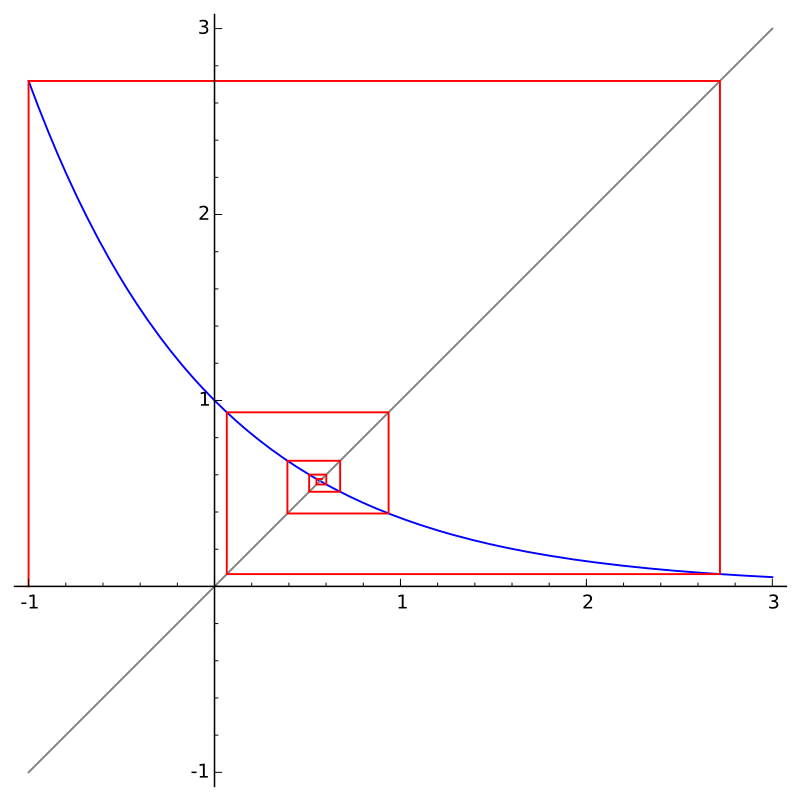
\includegraphics[scale=0.6]{figures/suites-visual1}
%\end{center}
%
%\begin{enumerate}
%  \item 
%On définit la fonction $f(x)=\exp(-x)$ par la commande \codeinline{f(x) = exp(-x)}.
%
%\insertcode{algos/suites-visual-tex1.sage}{suites-visual.sage (1)}
%
%Par exemple la commande \codeinline{liste_suite(f,-1,4)}
%calcule, pour $a=-1$, les $4$ premiers termes de la suite $(u_n)$ ;
%on obtient la liste :
%
%\centerline{\codeinline{[-1, e, e^(-e), e^(-e^(-e))]}}
%
%correspondant aux termes : $u_0=-1$, $u_1 = e$,
%$u_2 = e^{-e}$ et $u_3 = e^{-e^{-e}}$, où l'on note $e=\exp(1)$.
%
%\item Nous allons maintenant calculer une liste de points.
%On démarre du point initial $(u_0,0)$,
%puis pour chaque rang on calcule deux points :
%$\big(u_k,f(u_k)\big)$ et $\big(u_{k+1},u_{k+1}\big)$.
%Notez que chaque élément de la liste est ici un couple $(x,y)$ de
%coordonnées.
%
%\insertcode{algos/suites-visual-tex2.sage}{suites-visual.sage (2)}
%
%
%Par exemple la commande \codeinline{liste_points(f,-1,3)}
%calcule, pour $a=-1$, le point initial $(-1,0)$ et les $3$ premiers 
%points de la visualisation de la suite $(u_n)$ ;
%on obtient la liste :
%
%\centerline{\codeinline{[(-1, 0), (-1, e), (e, e), (e, e^(-e)), (e^(-e), e^(-e))]}}
%
%
%\bigskip
%
%Il ne reste plus qu'à tracer le graphe de la fonction et construire
%la suite en traçant les segments reliant les points.
%
%\insertcode{algos/suites-visual-tex3.sage}{suites-visual.sage (3)}
%
%Par exemple la figure illustrant ce tp est construite par la commande
%\codeinline{dessine_suite(f,-1,10)}.
%
%\bigskip
%
%\item  (et 4.) Passons à la partie mathématique. Pour simplifier l'étude on va supposer 
%$a=-1$. Donc $u_0=-1$ et $u_1=f(u_0)=\exp(1) = e$.
%\begin{enumerate}
%  \item La fonction $f$ définie par $f(x)=\exp(-x)$ est décroissante.
%  Donc la fonction $g$ définie par $g(x) = f\big( f(x) \big)$ est croissante.
%  
%  \item La suite $(u_{2n})_{n\in\Nn}$ 
%  des termes de rangs pairs est croissante. En effet :
%  $u_2 = e^{-e} \ge -1= u_0$. Alors 
%  $u_4 = f \circ f( u_2 ) \ge f\circ f(u_0) = u_2$
%  car $f\circ f=g$ est croissante.
%  Puis par récurrence $u_6 = f \circ f (u_4) \ge f\circ f (u_2) = u_4$...
%  La suite $(u_{2n})$ est croissante. 
%
%  \item Comme $u_2 \ge u_0$ et que $f$ est décroissante alors $u_3 \le u_1$.
%  On démontre alors de la même façon que la suite 
%  $(u_{2n+1})_{n\in\Nn}$ des termes de rangs impairs est décroissante.
%  
%  \item Enfin, toujours par la même méthode et en partant de
%  $u_0 \le u_1$, on prouve que $u_{2n} \le u_{2n+1}$.
%  
%  \item La situation est donc la suivante :
%  $$u_0 \le u_2 \le \cdots \le u_{2n} \le \cdots \le u_{2n+1} \le \cdots \le u_3 \le u_1$$
%  
%  La suite $(u_{2n})$ est croissante et majorée par $u_1$, donc elle converge. Notons $\ell$
%  sa limite.
%  
%  La suite $(u_{2n+1})$ est décroissante et minorée par $u_0$, donc elle converge. Notons $\ell'$
%  sa limite.
%  
%  \item Par les théorèmes usuels d'analyse, la suite $(u_{2n})$
%  converge vers un point fixe de la fonction $g=f \circ f$, 
%  c'est-à-dire une valeur $x_0$ vérifiant $f\circ f(x_0)=x_0$.
%  Une étude de la fonction $g$ (ou plus précisément de $g(x)-x$) montrerait que $g$
%  n'a qu'un seul point fixe. Voici le graphe de $g$.
%  \begin{center}
%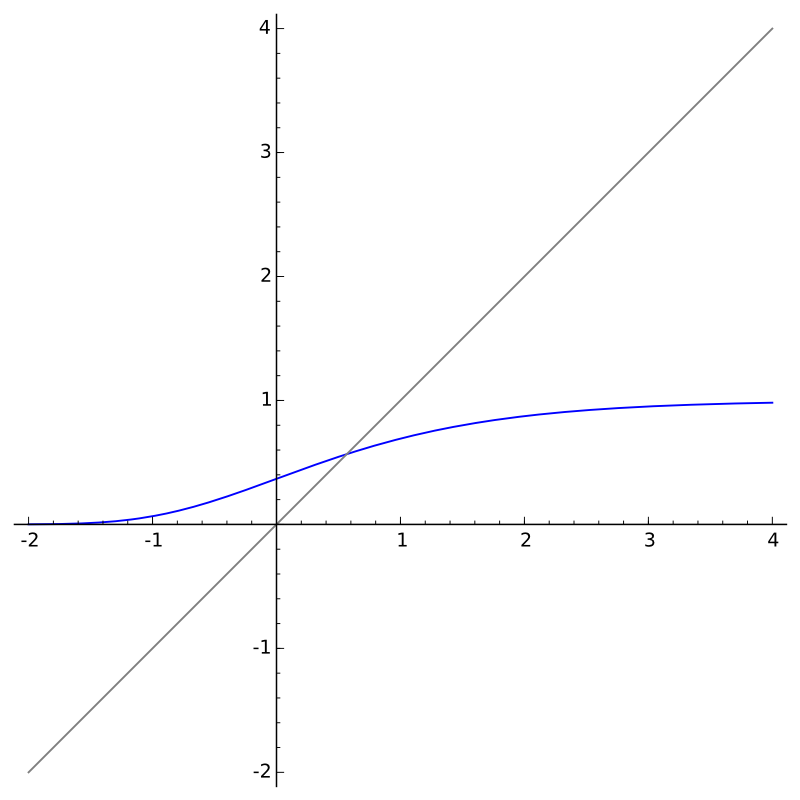
\includegraphics[scale=0.4]{figures/suites-visual2}
%\end{center} 
%
%  Cela prouve en particulier que $\ell=\ell'$.
%
%
%  \item  Par ailleurs la fonction $f$ admet un unique point fixe $x_0$.
%  Mais comme $f(x_0)=x_0$ alors l'égalité $f\big( f(x_0) \big) = f\big(x_0\big) = x_0$
%  prouve que $x_0$ est aussi le point fixe de $g$.
%  
%  \item Conclusion : la suite $(u_{2n})$ et la suite $(u_{2n+1})$ convergent
%  vers $x_0=\ell=\ell'$. Ainsi la suite $(u_n)$ converge vers $x_0$ le point fixe de $f$.
%
%  
%  \item Il n'y a pas d'expression simple de la solution $x_0$ de l'équation $f(x)=x$.
%  La commande \codeinline{solve(f(x)==x,x)} renvoie seulement l'équation.
%  Par contre, on obtient une valeur numérique approchée par
%  \codeinline{find_root(f(x)==x,0,1)}. On trouve $x_0 = 0,56714329041\ldots$
%  
%\end{enumerate}
%\end{enumerate}
%
%
%%--------------------------------------------------------
%\subsection{Listes}
%
%Une \defi{liste} est ce qui ressemble le plus à une suite mathématique.
%Une liste est une suite de nombres, de points\ldots ou même de listes !
%
%\begin{itemize}
%  
%  \item Une liste est présentée entre crochets :
%  \codeinline{mesprems = [2,3,5,7,11,13]}. 
%  On accède aux valeurs par \codeinline{mesprems[i]} ;
%  \codeinline{mesprems[0]} vaut $2$,  \codeinline{mesprems[1]} vaut $3$\ldots
%  
%
%  \item On parcourt les éléments d'une liste avec \codeinline{for p in mesprems:}, 
%  $p$ vaut alors successivement $2$, $3$, $5$, $7$\ldots
%  
%  \item Une première façon de créer une liste est de partir de la liste vide, 
%  qui s'écrit \codeinline{[]},
%  puis d'ajouter un à un des éléments à l'aide de la méthode \codeinline{append}. 
%  Par exemple \codeinline{mespoints=[]}, puis \codeinline{mespoints.append((2,3))},
%  \codeinline{mespoints.append((7,-1))}. La liste \codeinline{mespoints} contient alors deux
%  éléments (ici deux points)  \codeinline{[ (2,3), (7,-1) ]}.
%
%\end{itemize}
%  
%\begin{tp}
%Pour $n$ un entier fixé. Composer les listes suivantes :
%\begin{enumerate}
%  \item la liste des entiers de $0$ à $n-1$,
%  
%  \item la liste des entiers premiers strictement inférieurs à $n$,
%  
%  \item la liste des $2p+1$, pour les premiers $p$ strictement inférieurs à $n$,
%  
%  \item les $10$ premiers éléments de la liste précédente,
%    
%  \item la liste de $p_i+i$, où $(p_i)_{i\ge0}$ sont les nombres premiers 
%  strictement inférieurs à $n$ ($p_0=2$, $p_1=3$,...),
%  
%  \item la liste de $1$ et $0$ selon que le rang $0\le k <n$ soit premier ou pas.
%\end{enumerate} 
%\end{tp}
%
%
%Une utilisation intelligente permet un code très court et très lisible.
%Il faut potasser le manuel afin de manipuler les listes avec aisance.
%\begin{enumerate}
%  \item \codeinline{entiers = range(n)}
%  \item \codeinline{premiers = [k for k in range(n) if is_prime(k)]} 
%  \item \codeinline{doubles = [2*p+1 for p in premiers]}
%  \item \codeinline{debut = doubles[0:10]}
%  \item \codeinline{premiersplusrang = [premiers[i]+i for i in range(len(premiers))]}
%  \item \codeinline{binaire = [zeroun(k) for k in range(n)]} 
%  où \codeinline{zeroun(k)} est une fonction à définir qui renvoie $1$ ou $0$ 
%  selon que $k$ est premier ou pas. 
%\end{enumerate}
%
%On peut aussi trier les listes, les fusionner...
%
%% 
%% %--------------------------------------------------------
%% \subsection{La constante de Champernowne [à virer ?]}
%% 
%% Le tp suivant peut être passé lors d'une première lecture.
%% 
%% \begin{tp}
%% La constante de Champernowne
%% est 
%% $$\tau  = 0,0123456789\ 000102030405060708091011121314\ldots $$
%% Les décimales sont formées de tous les nombres à $1$ chiffres ($0,1,2,\ldots,9$), puis tous les nombres
%% à $2$ chiffres($00,01,2,\ldots,99$), puis tous les nombres à $3$ chiffres,... 
%% 
%% \begin{enumerate}
%%   \item \'Ecrire une fonction qui renvoie le réels
%%   $\tau_k$, dont les décimales sont formées des entiers de $1$ à $k$ chiffres.
%%   
%%   \item \'Ecrire une fonction qui renvoie la partie fractionnaire $\{x\}$ d'un réel $x$ :
%%   $$\{x\} = x - E(x)$$
%%   où $E(x)$ désigne la partie entière.
%%   
%%   \item Soit $x\in \Rr$. Montrer que pour tout $\epsilon>0$, il existe $p$ tel que
%%   $$\big| \{x\} - \{10^p \tau\} \big| < \epsilon$$
%%  
%%  \item Faire le même travail avec la constante binaire de Champernowne, dont l'écriture binaire
%%  $$\sigma = 0,\ 0 \ 1 \ 00 \ 01 \ 10 \ 11 \ 000 \ 001 \ 010 \ldots$$
%%  formés de la juxtaposition des entiers en écriture binaires à $1$, $2$, $3$,\ldots chiffres.
%%  On note $\{x\}_2$ la partie fractionnaire d'un réel en écriture binaire.
%%  Montrer que, quelque soit $x\in\Rr$, quelque soit $\epsilon>0$, il existe $p$ tel que
%%   $$\big| \{x\}_2 - \{2^p \tau\}_2 \big| < \epsilon$$
%% \end{enumerate}
%% \end{tp}
%
%
%%--------------------------------------------------------
%\subsection{Suites et chaos}
%
%
%\begin{tp}
%On considère la fonction $f$ définie sur $x \in [0,1]$ par 
%$$f(x)=rx(1-x) \qquad \text{ où } \quad 0 \le  r \le 4.$$
%
%Pour $r$ fixé et $u_0 \in [0,1]$ fixé, on définit une suite $(u_n)$ par
%$$u_{n+1} = f(u_n).$$
%
%\begin{enumerate}
%  \item Pour différentes valeurs de $r$ et $u_0$ fixées, tracer sur un même graphique
%  le graphe de $f$, la droite d'équation $(y=x)$ et la suite $(u_n)$. Essayez de conjecturer 
%  le comportement de la suite pour $0<r\le3$, $3< r \le 1+\sqrt{6}$,
%  $1+\sqrt{6}< r < 4$ et $r=4$. 
%  
%  \item Pour $u_0$ fixé et $M<N$ grands (par exemple $M=100$, $N=200$) tracer le \defi{diagramme
%  de bifurcation} de $f$, c'est-à-dire l'ensemble des points
%  $$(u_i,r) \qquad \text{ pour } \quad M \le i \le N \text{ et } 0 \le r \le 4$$
%  
%  \item 
%  \begin{enumerate}
%    \item Montrer que les points fixes de $f$ sont $0$ et $\frac{r-1}{r}$.
%    \item Montrer que le point fixe $0$ est répulsif (c'est-à-dire $|f'(0)|>1$) dès que $r>1$.
%    \item Montrer que le point fixe $\frac{r-1}{r}$ est attractif (c'est-à-dire $|f'(\frac{r-1}{r})|<1$)
%    si et seulement si $1< r < 3$. 
%  \end{enumerate}  
%  
%  
%  \item \textbf{Cas $1 < r \le3$. Pour $0<u_0<1$ la suite $(u_n)$ converge vers $\frac{r-1}{r}$.}
% 
%  On va prouver ce résultat seulement dans le cas particulier $r=2$ :
%  \begin{enumerate}
%    \item Montrer que $u_{n+1}-\frac12 = -2\left(u_n-\frac12\right)^2$.
%    \item Montrer que si $|u_0-\frac12| < k < \frac12$ alors 
%    $|u_n-\frac12| < \frac12 (2k)^{2^n}$.
%    \item Conclure.
%  \end{enumerate} 
%  
%  \item \textbf{Cas $3<r<1+\sqrt{6}$. La suite $(u_n)$ possède un cycle attracteur de période $2$.}
%   
%  \begin{enumerate}
%    \item Déterminer les points fixes $\ell_1$ et $\ell_2$ de $f\circ f$ qui ne sont pas des points fixes 
%    de $f$.
%     
%    \item Montrer que $f(\ell_1) = \ell_2$ et $f(\ell_2)=\ell_1$.
%     
%    \item \`A l'aide du graphe de $f\circ f$, vérifier graphiquement sur un exemple, 
%    que les suites $(u_{2n})$ et $(u_{2n+1})$ sont croissantes ou décroissantes à partir d'un certain rang
%    et convergent, l'une vers $\ell_1$, l'autre vers $\ell_2$.
%  \end{enumerate} 
%  
%  
%  \item \textbf{Cas $1+\sqrt{6}<r<3, 5699456\ldots$ La suite $(u_n)$ possède 
%  un cycle attracteur de période $4,8,16...$}
%  
%  Trouver de tels exemples.    
%  
%  \item \textbf{\`A partir de $r > 3, 5699456\ldots$ la suite $(u_n)$ devient chaotique.}
%\end{enumerate}
%\end{tp}
%
%
%Le tp suivant sera consacré au cas $r=4$.
%
%
%\begin{enumerate}
%  \item 
%  Voici le comportement de différentes suites définies par le même $u_0=0,123$ et pour $r$ valant 
%  successivement $r=2,2$, $r=3,2$, $r=3,57$ et $r=4$.
%  \begin{center}
%  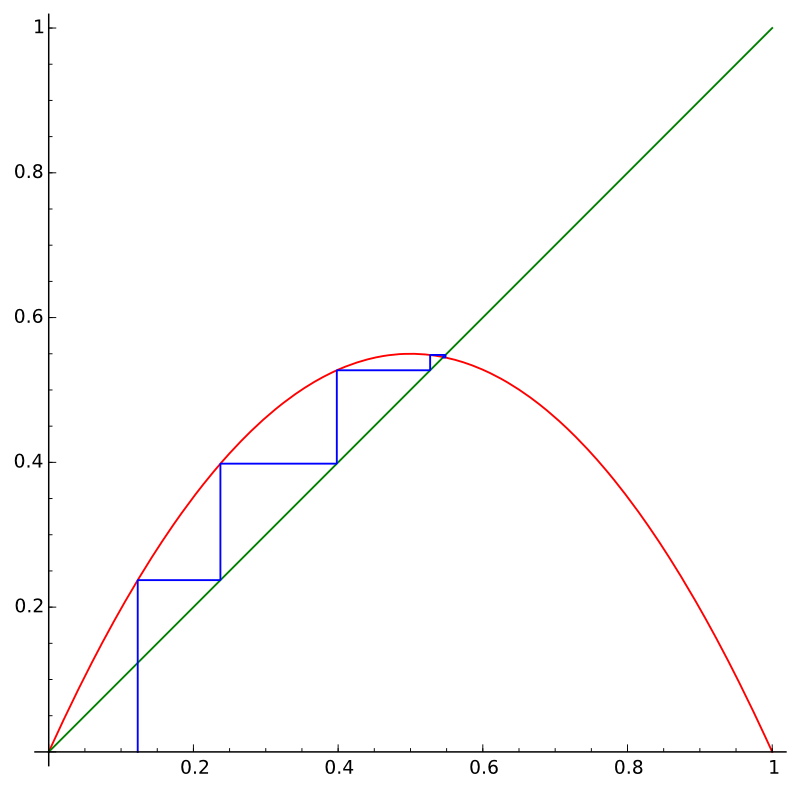
\includegraphics[scale=0.3]{figures/chaos1}\quad
%  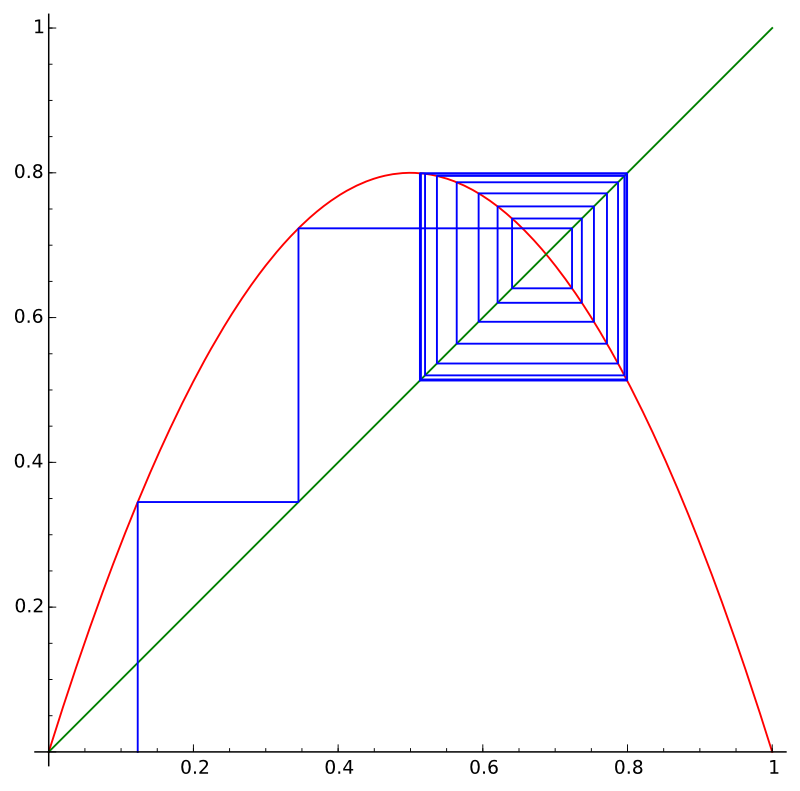
\includegraphics[scale=0.3]{figures/chaos2}\\[3mm]
%  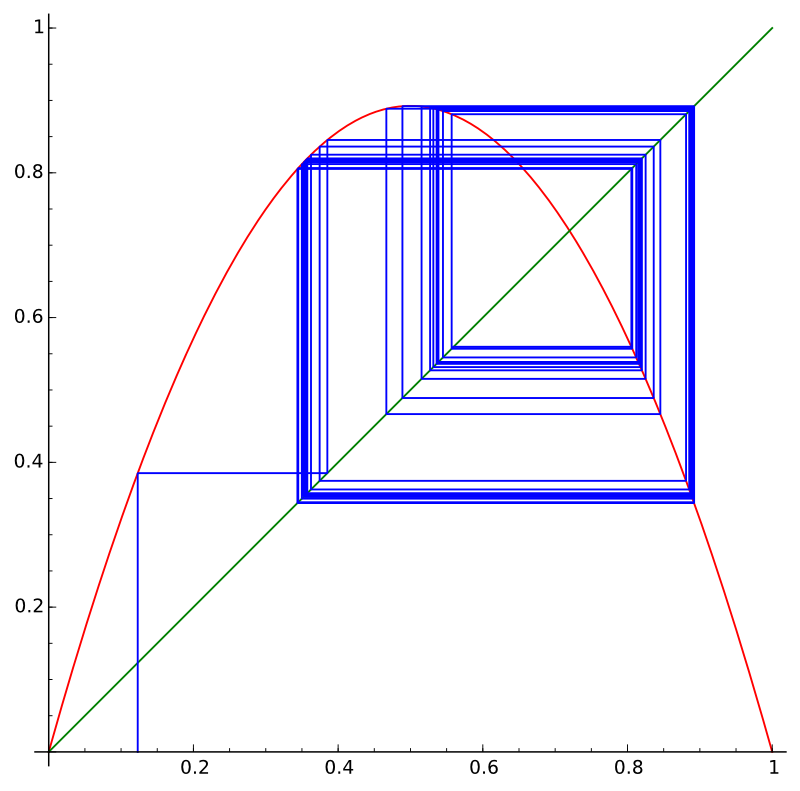
\includegraphics[scale=0.3]{figures/chaos3}\quad
%  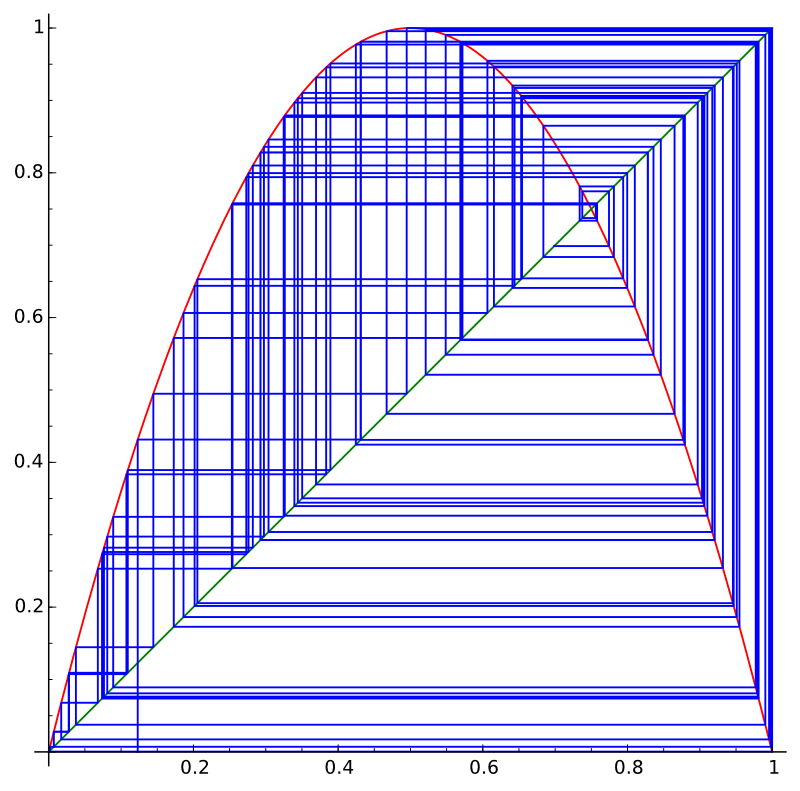
\includegraphics[scale=0.3]{figures/chaos4}  
%  \end{center}
%  On voit d'abord une limite, puis la suite semble avoir \og deux limites \fg\ c'est-à-dire
%  deux valeurs d'adhérence, puis $4$ valeurs d'adhérence. Pour 
%  $r=4$ la situation semble chaotique.
%  
%  
%  
%  \item Voici le code et le résultat.
%  
%  \insertcode{algos/suites-chaos-tex1.sage}{suites-chaos.sage (1)}
%  
%  \begin{center}
%  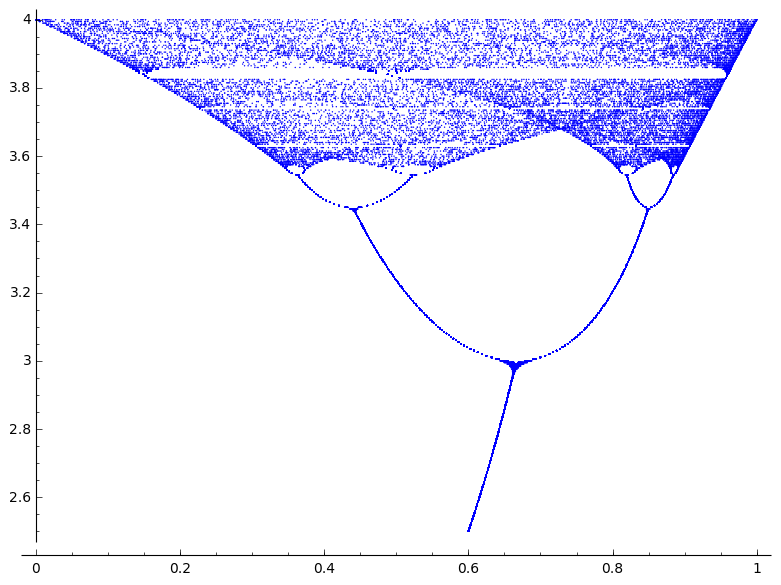
\includegraphics[scale=0.7]{figures/chaos5}  
%  \end{center} 
%
%  \item Voici le code pour les trois questions.
%    
%  \insertcode{algos/suites-chaos-tex2.sage}{suites-chaos.sage (2)}
%
%  
%    \begin{enumerate}
%    \item Les deux points fixes fournis dans la liste \codeinline{pts_fixes}
%    sont $0$ et $\frac{r-1}{r}$. 
%    
%    \item On calcule la dérivée \codeinline{ff}, 
%    on l'évalue en $0$, on trouve $f'(0)=r$. Ainsi si $r>1$ alors
%    $|f'(0)|>1$ et le point $0$ est répulsif. 
%    
%    \item Par contre lorsque l'on résout l'inéquation $|f'(\frac{r-1}{r})|<1$, 
%    la machine renvoie les conditions $r>1$ et $r < 3$. 
%    Ainsi pour $1<r<3$, le point fixe $\frac{r-1}{r}$ est attractif.
%  \end{enumerate} 
%  
%  \item On pose d'abord \codeinline{r = 2}, alors le point fixe est $\frac{r-1}{r}= \frac12$.
%  \begin{enumerate}
%    \item Après simplification \codeinline{(r*u*(1-u) - 1/2) + 2*(u-1/2)^2} vaut $0$.
%    Autrement dit $u_{n+1}-\frac12 = -2(u_n-\frac12)^2$, quelque soit $u_n$.
%    \item C'est une simple récurrence :
%    $$\left|u_{n+1}-\frac12\right|  = 2 \left(u_n-\frac12\right)^2 
%    < 2\left(\frac12 (2k)^{2^n}\right)^2 = \frac12 (2k)^{2^{n+1}}.$$
%    \item Ainsi pour $u_0 \neq 0,1$, il existe $k$ tel que $|u_0-\frac12| < k < \frac12$
%    et la suite $(u_n)$ tend (très très) vite vers le point fixe $\frac12$.
%  \end{enumerate} 
%  
%  Avec $r=2$, en quelques itérations le terme de la suite 
%  n'est plus discernable de la limite $\frac12$ :
%  \begin{center}
%  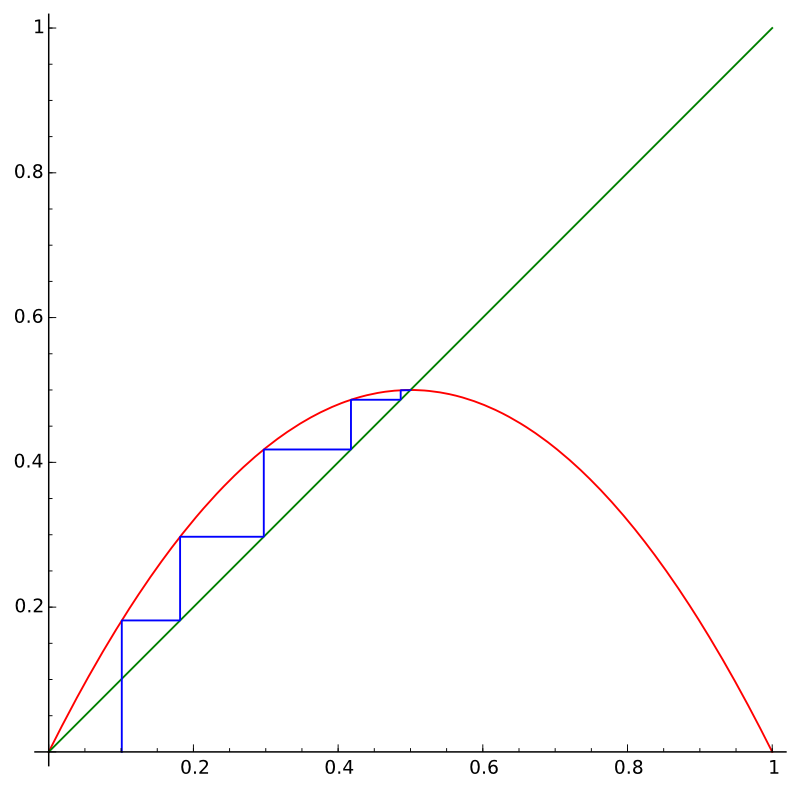
\includegraphics[scale=0.4]{figures/chaos6}  
%  \end{center}   
%  
%  \item  Voici le code pour les deux premières questions :
%  
%  \insertcode{algos/suites-chaos-tex3.sage}{suites-chaos.sage (3)}
%
%  \begin{enumerate}
%    \item On calcule les points fixes de $g = f\circ f$. Il y en a quatre, mais deux d'entre eux sont 
%    les points fixes de $f$. Les deux nouveaux sont :
%    $$\ell_1 = \frac12\frac{r + 1 - \sqrt{r^2 - 2r - 3}}{r} \qquad 
%      \ell_2 = \frac12\frac{r + 1 + \sqrt{r^2 - 2r - 3}}{r}$$
%      
%    \item Bien sûr $\ell_1$ et $\ell_2$ ne sont pas des points fixes pour $f$.
%    Par contre, on vérifie que $f(\ell_1) = \ell_2$ et $f(\ell_2)=\ell_1$.
%     
%    \item Voici les dessins pour $r=1+\sqrt{5}$ et $u_0=\frac23$.
%    La suite $(u_{2n})$, qui est vue comme suite récurrente de fonction $g$,
%    est décroissante vers $\ell_1$ (figure de gauche).
%    La suite $(u_{2n+1})$, vue comme suite récurrente de fonction $g$,
%    est croissante vers $\ell_2$ (figure de droite).
%  \begin{center}
%  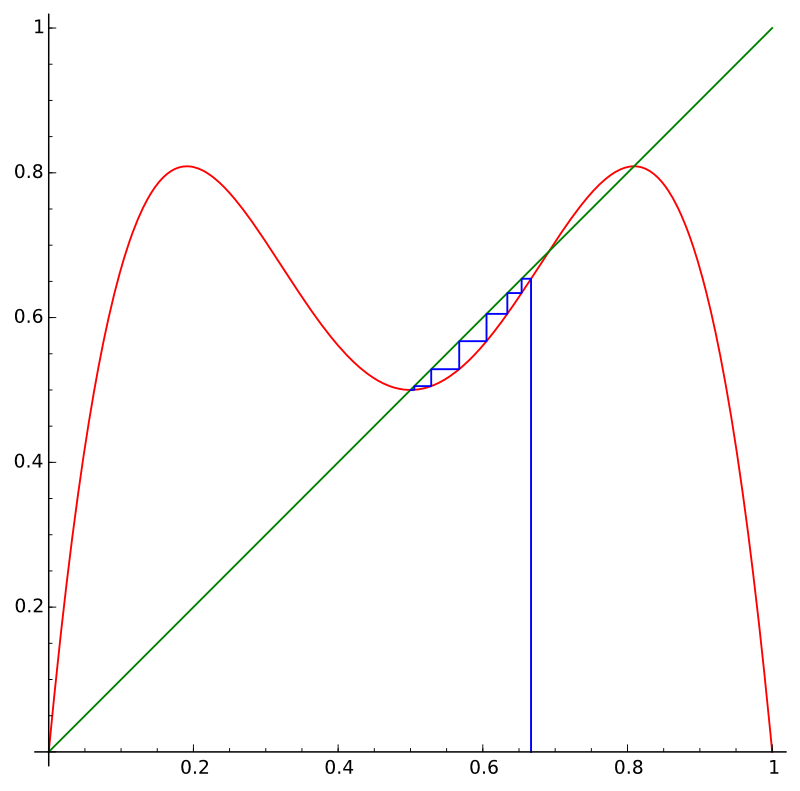
\includegraphics[scale=0.3]{figures/chaos7}\quad
%  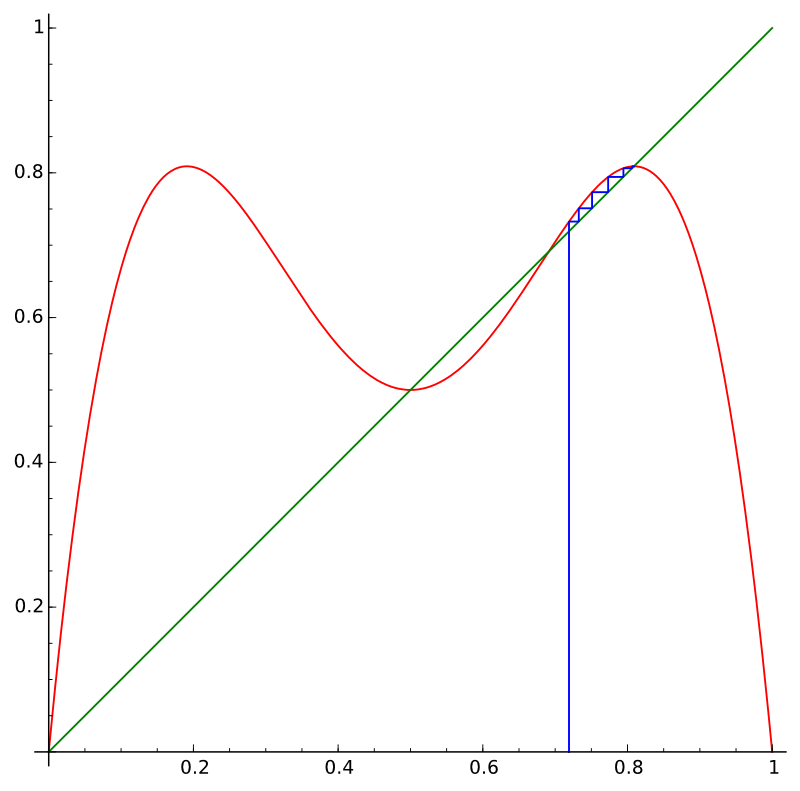
\includegraphics[scale=0.3]{figures/chaos8}
%  \end{center}
%  
%  La suite $(u_n)$, comme suite récurrente de fonction $f$, possède 
%  le cycle $(\ell_1,\ell_2)$ comme cycle attracteur :
%  \begin{center}
%  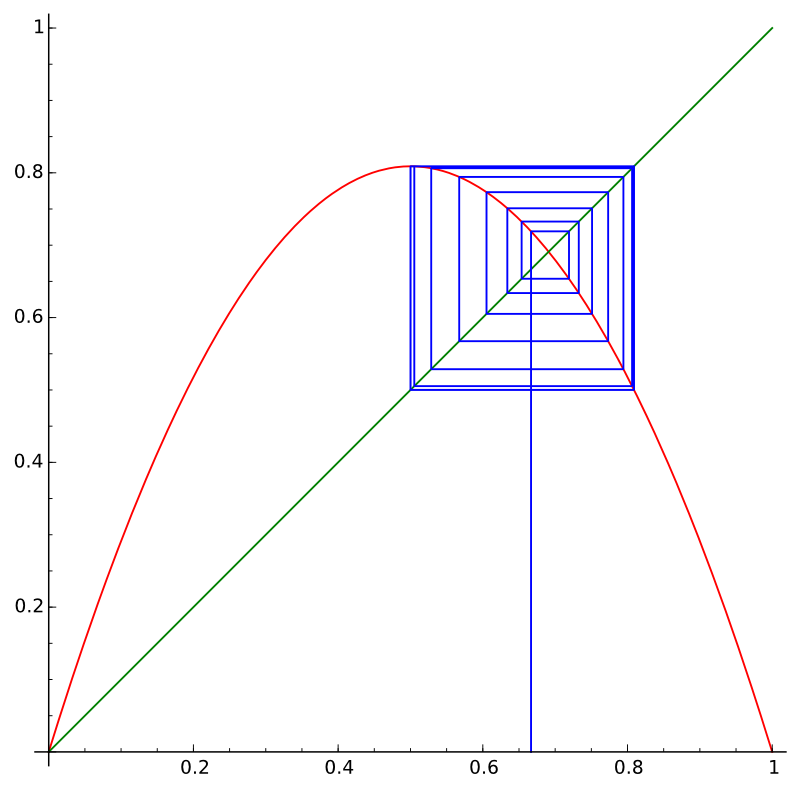
\includegraphics[scale=0.4]{figures/chaos9}
%  \end{center}
%  \end{enumerate} 
%  
%  \item Voici un exemple de cycle de longueur $8$ ($r=3,56$, $u_0=0,35$) :
%    \begin{center}
%  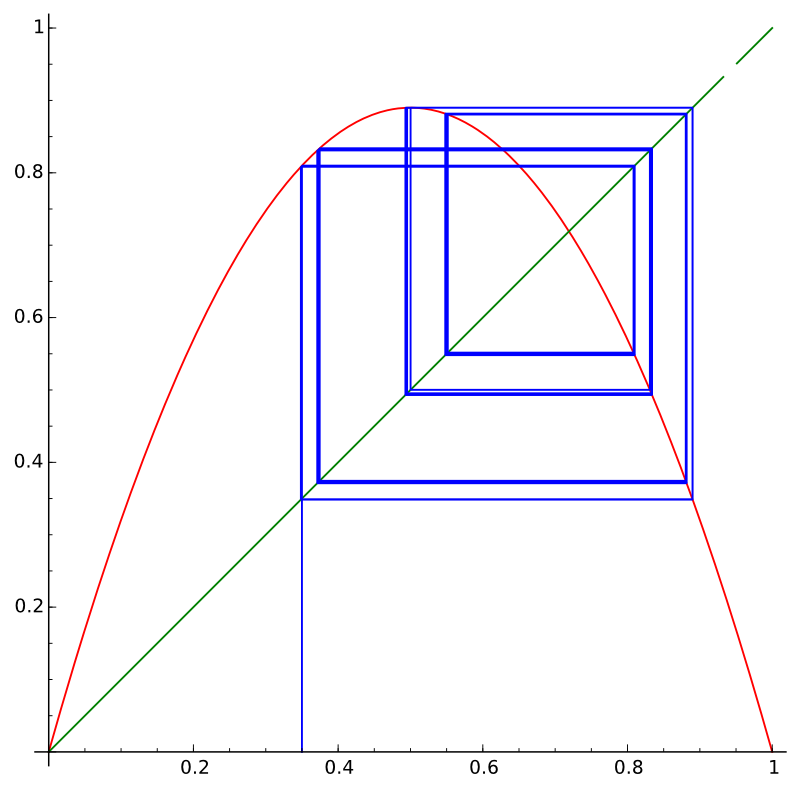
\includegraphics[scale=0.4]{figures/chaos10}
%  \end{center}
%  
%  \item Le cas $r=4$ sera étudié dans le tp suivant.
%      
%     
%\end{enumerate}
%
%
%\begin{tp}
%On s'intéresse au cas $r=4$. On rappelle que 
%$$f(x)=rx(1-x) \qquad u_0 \in [0,1] \qquad \mbox{et} \qquad u_{n+1} = f(u_n)\quad (n\geq 0).$$
%
%\begin{enumerate}
%  \item 
%  \begin{enumerate}
%    \item Montrer que $\sin^2(2t) = 4 \sin^2 t \cdot (1-\sin^2 t)$.
%    \item Montrer que pour $u_0 \in [0,1]$, il existe un unique $t \in [0,\frac\pi2]$ tel que
%    $u_0 = \sin^2 t$.
%    \item En déduire $u_n = \sin^2(2^n t)$.
%  \end{enumerate}
%  
%  \item Pour $t_k = \frac{2\pi}{2^k+1}$ et $u_0 = \sin^2 t_k$, 
%  montrer que la suite $(u_n)$ est périodique de période $k$.
%  
%  \item \textbf{La suite est instable.}
%  \begin{enumerate}
%    \item Pour $k=3$, on pose $t_3 = \frac{2\pi}{9}$, $u_0 = \sin^2 t_3$.
%    Calculer une valeur exacte (puis approchée) de $u_n$, pour tout $n$.
%    
%    \item Partant d'une valeur approchée $\tilde{u}_0$ de $u_0$, 
%    que donne la suite des approximations $(\tilde{u}_n)$ définie 
%    par la relation de récurrence ?
%  \end{enumerate}
%  
%    
%  \item \textbf{La suite est partout dense.}
%  
%  On va construire $u_0\in[0,1]$ tel que, tout $x\in[0,1]$ peut être approché d'aussi près que l'on veut par 
%  un terme $u_n$ de notre suite :
%  $$\forall x \in [0,1] \quad \forall \epsilon > 0 \quad \exists n \in \Nn \qquad \big| x -u_n \big| < \epsilon.$$
%  
%  
%  \begin{itemize}
%    \item Soit $\sigma$ la constante binaire de Champernowne, 
%    formée de la juxtaposition des entiers en écriture binaire 
%    à $1$, $2$, $3$,\ldots chiffres $0$, $1$, $00$, $01$, $10$,...
%    dont l'écriture binaire est $\sigma = 0,0100011011\ldots$
%    
%    \item Soit $u_0 = \sin^2 (\pi\sigma)$. 
%    
%    \item Soit $x \in [0,1[$. Ce réel peut s'écrire $x = \sin^2(\pi t)$ avec 
%    $t\in [0,1[$ qui admet une écriture binaire $t= 0,a_1 a_2 \ldots a_p \ldots$.
%  \end{itemize}
%  
%  Pour $\epsilon>0$ fixé, montrer qu'il existe $n$ tel que $\big| x -u_n \big| < \epsilon$.
%  
%\end{enumerate}
%
%\end{tp}
%
%\begin{enumerate}
%  \item 
%  \begin{enumerate}
%    \item On pose \codeinline{eq = sin(2*t)^2 - 4*sin(t)^2*(1-sin(t)^2)}
%    et \codeinline{eq.full_simplify()} renvoie $0$. Donc 
%    $\sin^2(2t) = 4 \sin^2 t \cdot (1-\sin^2 t)$, pour tout $t\in\Rr$.
%    
%    \item Soit $h(t) = \sin^2 t$. On définit la fonction \codeinline{h = sin(t)^2}, sa dérivée 
%    \codeinline{hh = diff(h,t)} dont on cherche les zéros 
%    par \codeinline{solve(hh==0,t)}. La dérivée ne s'annulant qu'en $t=0$ et
%    $t=\frac\pi2$. La fonction $h'$ est strictement monotone sur $[0,\frac\pi2]$.
%    Comme $h(0)=0$ et $h(\frac\pi2)=1$, pour chaque $u_0 \in [0,1]$, 
%    il existe un unique $t \in [0,\frac\pi2]$ tel que
%    $u_0 = h(t)$. 
%    \item Pour $u_0 = \sin^2 t$, on a 
%    $$u_{1} = f(u_0) = ru_0(1-u_0) = 4\sin^2 t \cdot (1-\sin^2 t) =  \sin^2(2 t).$$
%    On montre de même par récurrence que $u_n =   \sin^2(2^n t)$.
%  \end{enumerate}
%  
%  \item Le code suivant calcule $u_k-u_0$.
%  \Sage\ sait calculer que cela vaut $0$, pour $k$ prenant la valeur $0$, $1$, $2$,...
%  mais pas lorsque $k$ est une variable. Le calcul à la main est pourtant très simple !
%  
%    \insertcode{algos/suites-chaos-tex4.sage}{suites-chaos.sage (4)}
% 
%  \item \textbf{La suite est instable.}
%  \begin{enumerate}
%    \item  Pour $k=3$ et $t_3 = \frac{2\pi}{9}$, la suite $(u_k)$ est périodique de période $3$.
%    Donc il suffit de calculer $u_0,u_1,u_2$.
%    Par exemple :
%    $$u_{3p} = u_0 = \sin^2\left( \frac{2\pi}{9}\right) \simeq \num{0.4131759111\dots}$$
%    
%    \item Partons de la valeur approchée de $u_0$ avec $10$ décimales exactes :    
%    $\tilde{u}_0 = \num{0.4131759111}$ et calculons les premiers termes de la suite. On en extrait :
%
%\begin{center}
%\setlength{\arrayrulewidth}{0.05mm}
%\begin{tabular}{c} 
%%\begin{tabular}[t]{cc@{\vrule depth 2.5ex height 3.5ex width 0mm \ }} 
%$\tilde{u}_0\simeq $    \num{0.413175911100} \\
%$\tilde{u}_3\simeq $    \num{0.413175911698} \\
%$\tilde{u}_6\simeq $    \num{0.413175906908} \\
%$\tilde{u}_9\simeq $    \num{0.413175945232} \\
%$\tilde{u}_{12}\simeq $ \num{0.413175638640} \\
%$\tilde{u}_{15}\simeq $ \num{0.413178091373} \\
%$\tilde{u}_{18}\simeq $ \num{0.413158469568} \\
%$\tilde{u}_{21}\simeq $ \num{0.413315447870} \\
%$\tilde{u}_{24}\simeq $ \num{0.412059869464} \\
%$\tilde{u}_{27}\simeq $ \num{0.422119825829} \\
%$\tilde{u}_{30}\simeq $ \num{0.342897499745} \\
%$\tilde{u}_{33}\simeq $ \num{0.916955513784} \\
%$\tilde{u}_{36}\simeq $ \num{0.517632311613} \\
%$\tilde{u}_{39}\simeq $ \num{0.019774022431} \\
%\end{tabular} 
%\end{center} 
%
%Si l'approximation de départ et tous les calculs étaient exacts, on devrait obtenir
%$u_0$ à chaque ligne. On constate que l'erreur augmente terme après terme, 
%et après $\tilde{u}_{30}$, le comportement de $\tilde{u}_{n}$ 
%n'a plus rien à voir avec $u_n$.
%L'explication vient de la formule $u_n =   \sin^2(2^n t)$, une erreur 
%sur $t$, même infime au départ, devient grande par multiplication par $2^n$.
%
%  \end{enumerate}
%  
%    
%  \item \textbf{La suite est partout dense.}
%  
%  La construction est assez jolie mais délicate. (Il ne faut pas avoir peur de 
%  l'écriture en base $2$ qui n'est pas ici le point clé. 
%  Vous pouvez penser en base $10$ pour mieux comprendre.)
%  
%  
%  Fixons $\epsilon >0$. Soit un entier $p$ tel que 
%  $\frac{\pi}{2^p} < \epsilon$.
%  L'écriture binaire de $t$ étant $t= 0,a_1 a_2 \ldots a_p \ldots$
%  la séquence $a_1 a_2 \ldots a_p$ apparaît quelque part dans la constante de
%  Champernowne. Plus précisément il existe un entier $n$ tel que
%  $2^n \sigma = \ldots b_2b_1b_0,a_1 a_2 \ldots a_p\ldots$
%  (on a fait apparaître la séquence juste après la virgule par 
%  décalage de la virgule).
%  
%  On va pouvoir oublier la partie entière $m = \ldots b_2b_1b_0 \in \Nn$ et on note $\tilde \sigma 
%  = 0,a_1 a_2 \ldots a_p\ldots$ la partie fractionnaire de $\sigma$, 
%  de sorte que $\sigma = m + \tilde  \sigma$.
%  
%  \begin{align*}
%  |x-u_p| 
%    &= \left| \sin^2(\pi t) - \sin^2(2^p \pi \sigma)\right| \\
%   &= \left| \sin^2(\pi t) - \sin^2(2^p \pi m + \pi \tilde\sigma)\right| \\ 
%    &=   \left| \sin^2(\pi t) - \sin^2(\pi \tilde\sigma)\right| 
%      \qquad \text{ car $\sin^2$ est $\pi$-périodique}\\
%    &\le  \left| \pi t - \pi \tilde\sigma\right| 
%      \qquad \text{ par le théorème des accroissements finis}\\
%    &\le  \pi \frac1{2^p}  
%      \qquad \text{ car $t$ et $\tilde\sigma$ ont les mêmes $p$ premières décimales}\\
%    &< \epsilon
%  \end{align*}
%
%  Conclusion : n'importe quel $x$ est approché d'aussi près que 
%  l'on veut par la suite. 
%  
%\end{enumerate}
%
%
%\bigskip
%
%Pour en savoir plus : 
%\begin{itemize}
%  \item \href{http://www.math.u-psud.fr/~perrin/Conferences/logistiqueDP.pdf}
%  {\emph{La suite logistique et le chaos}}, Daniel Perrin.
%  
%  \item \href{http://www.casio-education.fr/calculatrice_casio_documents/exercices/classpad330/exo001.pdf}
%  {\emph{\'Etude d’une suite récurrente}}, Jean-Michel Ferrard.
%\end{itemize}
%
%
%
%
%
%
%% 
%% %%%%%%%%%%%%%%%%%%%%%%%%%%%%%%%%%%%%%%%%%%%%%%%%%%%%%%%%%%%%%%%%
%% \section{Calculs approchés d'intégrales}
%% 
%% Nous allons voir plusieurs méthodes pour calculer des intégrales. Nous verrons plus tard des 
%% méthodes de résolution exacte. 
%% Il arrive très souvent que l'on ne puisse calculer de façon exact les intégrales, 
%% c'est pourquoi nous commençons par exposer différentes façons 
%% d'obtenir des valeurs approchées d'une intégrale.
%% 
%% 
%% 
%% On souhaite trouver une valeur approchée de l'intégrale :
%% $$I = \int_a^b f(x)\;\dd x$$
%% Les méthodes d'approximation que vous allez étudier sont toutes basées sur
%% le même principe : 
%% \begin{itemize}
%%   \item On divise l'intervalle $[a,b]$ en $n$ sous-intervalles. 
%%   On pose $x_k = a + k \frac{b-a}{n}$ et $0\le k \le n$.
%%   Alors $x_0=a$ et $x_n = b$. Cela définit une subdivision régulière 
%%   composée de $n$ sous-intervalles $[x_k,x_{k+1}]$, $0 \le k < n$,
%%   chaque sous-intervalle a une longueur constante 
%%   $x_{k+1}-x_k= \frac{b-a}{n}$ que l'on note $\epsilon$.
%%   
%% \myfigure{1}{
%% \tikzinput{fig_formel_int09}
%% }  
%% 
%%   \item Sur chaque sous-intervalle $[x_k,x_{k+1}]$ on approche l'aire sous la courbe
%%   par l'aire d'une figure géométrique simple.
%% \end{itemize}
%% 
%% Nous allons tester nos approximations sur deux exemples :
%% \myfigure{1}{
%% \tikzinput{fig_formel_int01}\qquad
%% \tikzinput{fig_formel_int02}
%% } 
%% \begin{itemize}
%%   \item L'intégrale $$I = \int_0^2 \frac{\dd x}{1+x} = \big[ \ln(1+x) \big]_0^2 = \ln 3,$$ 
%%   ce qui nous permettra d'obtenir une valeur approchée de $\ln 3$.
%%   
%%   \item Le (quart du) périmètre d'une ellipse 
%%   $$J = \int_ 0^{\frac\pi2}  \sqrt{4 \sin^2 x + \cos^2 x}\;\dd x$$
%%   En effet la longueur d'une courbe paramétrée 
%%   $\big(x(t),y(t)\big)$, $t\in[a,b]$ est donnée par
%%   $\ell = \int_a^b  \sqrt{x'(t)^2+y'(t)^2} \;\dd t$.
%%   Ce qui donne bien la formule $J$ pour la paramétrisation de l'ellipse 
%%   $\big(x(t) = 2\cos t, y(t) =\sin t\big)$.
%% \end{itemize}
%% 
%% 
%% 
%% 
%% %--------------------------------------------------------
%% \subsection{Méthode des rectangles}
%% 
%% La méthode des rectangles à gauche consiste à approcher l'aire sous la courbe
%% par l'aire de rectangles. La hauteur de chaque rectangle est la valeur à gauche
%% de $f$ sur le sous-intervalle (c.f. rectangles ci-dessous).
%% Pour un intervalle élémentaire, cela revient à approcher
%% $\int_a^b f(x)\;\dd x$ par $(b-a) f(a)$.
%% 
%% \myfigure{1}{
%% \tikzinput{fig_formel_int03}\qquad
%% \tikzinput{fig_formel_int05}
%% } 
%% 
%% On définit de même une méthode de rectangles à droite, en approchant l'intégrale 
%% par $(b-a) f(b)$ 
%% (c.f. rectangles ci-dessous).
%% 
%% \myfigure{1}{
%% \tikzinput{fig_formel_int04}
%% \tikzinput{fig_formel_int06}
%% } 
%% 
%% \begin{tp}
%% \begin{enumerate}
%%   \item \'Ecrire une fonction qui met en \oe uvre 
%%   la méthode des rectangles à gauche ; 
%%   puis la méthode des rectangles à droites.
%%     
%%   \item 
%%   \begin{enumerate}
%%     \item Quel encadrement obtient-on si la fonction est décroissante ?
%%     \item Donner l'encadrement de $I = \int_0^2 \frac{\dd x}{1+x}$, par des rationnels, obtenu pour $n=5$. 
%%     \item Trouver une approximation à $10^{-3}$ de $\ln 3$ par des décimaux.
%%   \end{enumerate}
%%   
%%   \item Quelle approximation de $J = \int_ 0^{\frac\pi2}  \sqrt{4 \sin^2 x + \cos^2 x}\;\dd x$ obtient-on pour $n=10$ ?
%% \end{enumerate}  
%% \end{tp}
%% 
%% \begin{enumerate}
%%   \item L'aire d'un rectangle à gauche au-dessus de l'intervalle élémentaire $[x_k,x_{k+1}]$ est
%%   $\frac{b-a}{n} f(x_k)$. 
%%   La méthode des rectangles à gauche est l'approximation de l'intégrale par la somme
%%   $$S_G(n) = \frac{b-a}{n}\sum_{k=0}^{n-1} f(x_k).$$
%%   
%%   Voici le code :
%%   
%%   \insertcode{algos/approx-integrale-tex1.sage}{approx-integrale.sage (1)} 
%%   
%%   Notez que l'on ne calcule pas $x_k$ par la formule $x_k = a + k\frac{b-a}{n}$,
%%   (qui demande un addition, une multiplication et une division à chaque étape) 
%%   mais par la formule de récurrence $x_k = x_{k-1} + \epsilon$ où $\epsilon =  \frac{b-a}{n}$
%%   est calculé une fois pour toute (ce qui fait donc seulement une addition à chaque étape).
%%   
%%   La méthode des rectangles à droite est l'approximation de l'intégrale par la somme
%%   $$S_D(n) = \frac{b-a}{n}\sum_{k=1}^{n} f(x_k).$$
%%   Noter que l'indice $k$ varie ici de $1$ à $n$.
%%   
%%   \item  
%%   \begin{enumerate}
%%     \item Si la fonction est décroissante alors pour $x_k \le x \le x_{k+1}$ on a 
%%   $f(x_{k+1}) \le f(x) \le f(x_k)$, ainsi sur chaque intervalle élémentaire les rectangles
%%   à gauche et à droite encadre l'aire sous la courbe.
%%   
%%   
%% \myfigure{1}{
%% \tikzinput{fig_formel_int10}
%% }   
%%   
%%   Ceci correspond à l'approximation 
%%   $\frac{b-a}{n}f(x_{k+1}) \le \int_{x_k}^{x_{k+1}} f(x) \;\dd x \le \frac{b-a}{n}f(x_k) $.
%%   Lorsque l'on fait la somme pour $k=0,\ldots,n-1$, on obtient
%%   $$S_D(n) \le  \int_a^b f(x)\;\dd x\le S_G(n)$$
%%   
%%     \item Pour $n=5$ et $I = \int_0^2 \frac{\dd x}{1+x} = \ln 3$, on obtient :
%%     $$\num{0.97\dots} = \frac{44006}{45045} \le \ln 3 \le \frac{56018}{45045} = \num{1.24\dots}$$
%%     
%%     \item Pour $n=2000$, on obtient $S_D(2000) = \num{1.0982\dots} \le \ln 3 \le S_G(2000) 
%%     = \num{1.0989\dots}$
%%     Ainsi $S_G(2000)-S_D(2000) \le \num{0.001}$. Et ainsi $\big|\ln 3 - \num{1.098}\big| \le 10^{-3}$.
%%     
%%   \end{enumerate}
%%   
%%   
%%   \item Cette fois la fonction $f(x) = \sqrt{4 \sin^2 x + \cos^2 x}$ est croissante.
%%   Les rectangles à gauche sont plus petits que les rectangles à droite. 
%%   Pour l'approximation de $J$ avec $n=10$ on obtient :  
%%   $$ \num{2.343} \le  J \le \num{2.500}$$
%%   
%% \end{enumerate}
%% 
%% \bigskip
%%   
%% En fait une majoration de l'erreur est donnée par le résultat suivant.
%% \begin{proposition}
%% Soit $f : [a,b] \to \Rr$ une fonction de classe $C^1$ ; soit $M_1 = \sup_{x\in[a,b]} \big|f'(x)\big|$.
%% Soit $S_G(n) = \frac{b-a}{n}\sum_{k=0}^{n-1} f(x_k)$ la somme des rectangles à gauche.
%% Alors 
%% $$\big| I - S_G(n) \big| \le \frac{(b-a)^2}{2n} M_1$$
%% \end{proposition}
%% 
%% Par exemple pour le calcul de notre intégrale $I$,
%% on sait que $\big| f'(x) \big| = \left| \frac{-1}{(1+x)^2} \right| \le 1 = M_1$.
%% On cherche les $n$ tels que $\frac{(b-a)^2}{2n} M_1 \le 10^{-3}$.
%% 
%% Tout se fait très bien à la main, mais on peut demander à \Sage\ de 
%% faire le calcul pour nous :
%% \begin{itemize}
%%   \item Par exemple en posant \codeinline{ff = abs(diff(f,x))}
%% alors la commande \codeinline{ff.find_local_maximum(a,b)}
%% nous indique numériquement que $|f'(x)| \le 1$. 
%% 
%%   \item Puis on cherche les $n$ valides en résolvant une inéquation :\\
%%   \centerline{\codeinline{solve( (b-a)^2/(2*n) <= 10^(-3), n )}}
%%   ce qui conduit à $n\ge 2000$.
%% \end{itemize}
%% 
%% 
%% %--------------------------------------------------------
%% \subsection{Méthode des trapèzes}
%% 
%% 
%% Vous allez faire le même travail pour la méthode des trapèzes.
%% On approche l'aire sous la courbe d'un intervalle élémentaire, 
%% par l'aire d'un trapèze.
%% 
%% \myfigure{1}{
%% \tikzinput{fig_formel_int07}
%% } 
%% 
%% \begin{tp}\sauteligne
%% \begin{enumerate}
%%   \item Calculer l'aire du trapèze correspondant au dessin ci-dessus. 
%%   \'Ecrire une fonction qui met en \oe uvre   la méthode des trapèzes.
%%   
%%   \begin{enumerate}
%%     \item Donner l'approximation de $I = \int_0^2 \frac{\dd x}{1+x}$, par un rationnel, obtenue pour $n=5$. 
%%  
%%     \item Trouver une approximation à $10^{-3}$ de 
%%     $\ln 3$ par des décimaux.
%%   \end{enumerate}
%%   
%%   \item Quelle approximation de $J = \int_ 0^{\frac\pi2}  \sqrt{4 \sin^2 x + \cos^2 x}\;\dd x$ obtient-on pour $n=10$ ?
%% \end{enumerate}  
%% \end{tp}
%% Pour prouver les approximations vous aurez besoin de la 
%% majoration de l'erreur donnée par le résultat suivant.
%% \begin{proposition}
%% Soit $f : [a,b] \to \Rr$ une fonction de classe $C^2$ ; soit $M_2 = \sup_{x\in[a,b]} \big|f''(x)\big|$.
%% Soit $S_T(n) = \frac{b-a}{n}\sum_{k=0}^{n-1} \frac{f(x_k)+f(x_{k+1})}{2}$ la somme des trapèzes.
%% Alors 
%% $$\big| I - S_T(n) \big| \le \frac{(b-a)^3}{12n^2} M_2.$$
%% \end{proposition}
%% 
%% Notez le progrès par rapport à la méthode des rectangles, le dénominateur contient le terme en $n^2$.
%% Donc l'erreur tend beaucoup plus vite vers $0$, lorsque $n$ tend vers $+\infty$.
%% 
%% 
%% \begin{enumerate}
%%   \item L'aire d'un trapèze au-dessus de l'intervalle élémentaire $[x_k,x_{k+1}]$ est
%%   $\frac{b-a}{n} \frac{f(x_k)+f(x_{k+1})}{2}$. Ce qui donne la somme
%%   $$S_T(n) = \frac{b-a}{n}\sum_{k=0}^{n-1} \frac{f(x_k)+f(x_{k+1})}{2}.$$
%%   
%%   L'implémentation est donc similaire à celle des rectangles en changeant une ligne en \\
%%   \centerline{\codeinline{somme = somme + (f(xk)+f(xk+epsilon))/2}}
%%   
%%   (C'est un bon exercice de réécrire la fonction de sorte qu'elle n'évalue $f(x_k)$ qu'une seule fois, et 
%%   pas deux fois comme dans la boucle ci-dessus.)
%%   
%%   
%%   \item
%%   \begin{enumerate}
%%     \item Pour $n=5$ on trouve $I = \ln 3 \simeq \frac{50012}{45045} = \num{1.1102\dots}$.
%%     Pour savoir quelle est la précision de cette approximation, nous majorons l'erreur commise.
%%     Comme $f''(x) = \frac{2}{(x+1)^3}$. Alors $M_2 = 2$.
%%     Pour $n = 5$ :
%%     $$\big| I - S_T(n) \big| \le \frac{(b-a)^3}{12n^2} M_2 = \frac{2}{75} = \num{0.02666\dots}$$
%% 
%%     
%%     \item Pour être sûr d'avoir une erreur inférieure à $10^{-3}$, il suffit de choisir
%%     $n$ de sorte que  $\frac{(b-a)^3}{12n^2} M_2 \le 10^{-3}$.
%%     On trouve ici que dès que $n \ge 37$, l'erreur est moindre
%%     que $10^{-3}$.
%%     
%%   \end{enumerate}
%%    
%%   \item Pour le calcul de $J$ et $n= 10$ on obtient :
%%   $$J \simeq S_T(10) = \num{2.42211\dots}$$
%%   
%%   Pour savoir l'erreur maximale commise, on étudie la fonction 
%%   $f(x) = \sqrt{4 \sin^2 x + \cos^2 x}$. on demande à \Sage\ de majorer la dérivée seconde $f''$
%%   définie  par \codeinline{diff(f,x,2)} :\\
%%   \centerline{\codeinline{ff = abs(diff(f,x,2))} puis \codeinline{ff.find_local_maximum(a,b)}}
%%   On trouve que le maximum est $M_2 = \frac{3}{2}$.
%%   Donc pour $n=10$, on trouve 
%%   $$\big| J - S_T(10) \big| \le \num{0.00484\dots}$$
%%   
%%   L'erreur $\big| J - S_T(10) \big|$ est en fait bien moindre que l'erreur maximale calculée.
%%    
%% \end{enumerate}
%% 
%% %--------------------------------------------------------
%% \subsection{Méthode de Simpson}
%% 
%% La méthode de Simpson consiste à approcher la courbe sur chaque intervalle élémentaire
%% par une branche de parabole. 
%% \myfigure{1}{
%% \tikzinput{fig_formel_int08}
%% } 
%% Cette parabole est la parabole passant par les trois
%% points de la courbe  : 
%% \begin{itemize}
%%   \item $\big( a, f(a) \big)$,
%%   \item $\big( b, f(b) \big)$,
%%   \item et le point dont l'abscisse est le milieu :
%% $\big( \frac{a+b}{2}, f\left( \frac{a+b}{2}\right)\big)$.
%% \end{itemize}
%% 
%% Il se trouve que l'aire sous cette portion de parabole se calcule très facilement,
%% c'est :
%% $$\frac{b-a}{6} \left( f(a)+f(b) + 4f\left(\frac{a+b}{2}\right) \right)$$
%% 
%% 
%% \begin{tp}\sauteligne
%% \begin{enumerate}
%%   \item \'Ecrire une fonction qui met en \oe uvre  la méthode de Simpson.
%%   
%%   \begin{enumerate}
%%     \item Donner l'approximation de $I = \int_0^2 \frac{\dd x}{1+x}$, par un rationnel, obtenue pour $n=5$. 
%%  
%%     \item Trouver une approximation à $10^{-10}$ de 
%%     $\ln 3 = \int_0^2 \frac{\dd x}{1+x}$ par des décimaux.
%%   \end{enumerate}
%%   
%%   \item Quelle approximation de $J = \int_ 0^{\frac\pi2}  \sqrt{4 \sin^2 x + \cos^2 x}\;\dd x$ obtient-on pour $n=10$ ?
%% \end{enumerate}  
%% \end{tp}
%% 
%% 
%% Voici l'erreur maximale commise par la méthode de Simpson.
%% \begin{proposition}
%% Soit $f : [a,b] \to \Rr$ une fonction de classe $C^4$ ; soit $M_4 = \sup_{x\in[a,b]} \big|f^{(4)}(x)\big|$.
%% Soit 
%% $$S_S(n) = \frac{b-a}{6n}\sum_{k=0}^{n-1} f(x_k)+f(x_{k+1})+4f\left(\frac{x_k+x_{k+1}}{2}\right)$$
%% la somme de Simpson.
%% Alors 
%% $$\big| I - S_S(n) \big| \le \frac{(b-a)^5}{2880n^4} M_4.$$
%% \end{proposition}
%% C'est encore mieux que les méthodes précédentes, grâce au terme en $n^4$ au dénominateur.
%% 
%% 
%% \begin{enumerate}
%%   \item La somme pour la méthode de Simpson est
%%   $$S_S(n) = \frac{b-a}{6n}\sum_{k=0}^{n-1} 
%%   f(x_k)+f(x_{k+1})+4f\left(\frac{x_k+x_{k+1}}{2}\right).$$
%%   
%%   L'implémentation est donc similaire aux précédentes avec \\
%%   \centerline{\codeinline{somme = somme +  f(xk)+f(xk+epsilon)+4*f(xk+epsilon/2)}}
%%   et en renvoyant à la fin \codeinline{(b-a)/(6*n)*somme}.
%%  
%%   
%%   \item
%%   \begin{enumerate}
%%     \item Pour $n=5$ on trouve $I = \ln 3 \simeq \frac{59387}{54054} \simeq \num{1.09866059866060\dots}$.
%%     On calcule $M_4 = 24$, donc pour $n = 5$ :
%%     $$\big| I - S_S(n) \big| \le \frac{(b-a)^5}{2880n^4} M_4 = \num{0.000085333\dots}$$
%%     L'erreur est donc déjà inférieure à $10^{-4}$.
%%     
%%     \item Pour être sûr d'avoir une erreur inférieure à $10^{-10}$ il suffit de choisir
%%     $n$ de sorte que  $\frac{(b-a)^5}{2880n^4} M_4 \le 10^{-10}$.
%%     Ce qui est vrai dès que $n \ge 228$, ce qui donne :
%%     $$I \simeq \num{1.0986122886\dots}$$
%%     
%%   \end{enumerate}
%%    
%%   \item  Pour le calcul de $J$ et $n = 10$ on obtient :
%%   $$J \simeq S_S(10) = \num{2.42211205513\dots}$$
%%   
%%   Pour savoir l'erreur maximale commise, on majore la dérivée quatrième $f^{(4)}$ par
%%   $M_4 \le 10$.  Donc pour $n=10$, on trouve 
%%   $$\big| J - S_S(10) \big| \le 10^{-5}.$$
%%   
%%   Encore une fois l'erreur $\big| J - S_S(10) \big|$ est bien moindre 
%%   que l'erreur maximale calculée.
%%    
%% \end{enumerate}
%% 
%% %--------------------------------------------------------
%% \subsection{Résumé}
%% 
%% Comparons l'efficacité des trois méthodes :
%% les rectangles (à gauche ou à droite), les trapèzes, la méthode de Simpson.
%% 
%% \myfigure{0.7}{
%% \tikzinput{fig_formel_int05}\qquad\qquad
%% \tikzinput{fig_formel_int07}\qquad
%% \tikzinput{fig_formel_int08}
%% } 
%% 
%% Soit une fonction $f : [a,b] \to \Rr$ pour laquelle on souhaite calculer
%% une valeur approchée de 
%% $$I = \int_a^b f(x)\;\dd x.$$
%% On suppose que $f$ est suffisamment dérivable et on note 
%% $$M_k = \sup_{x\in[a,b]} \big| f^{(k)}(x) \big|.$$
%% 
%% \begin{center}
%% \setlength{\arrayrulewidth}{0.05mm}
%% %\begin{tabular}{|l|l|l|} \hline
%% \begin{tabular}[t]{ccc@{\vrule depth 2.5ex height 3.5ex width 0mm \ }} 
%%   \quad Méthode \qquad  & Somme                         & Erreur \\ \hline\hline
%%    Rectangles           & $\displaystyle S_G(n) = \frac{b-a}{n}\sum_{k=0}^{n-1} f(x_k)$      
%%    & $\displaystyle \frac{(b-a)^2}{2n} M_1$ \\ \hline
%%    Trapèzes             &   $\displaystyle S_T(n) = \frac{b-a}{n}\sum_{k=0}^{n-1} \frac{f(x_k)+f(x_{k+1})}{2}$  
%%    & $\displaystyle \frac{(b-a)^3}{12n^2} M_2$ \\ \hline
%%    Simpson              &  
%%    $\displaystyle S_S(n) = \frac{b-a}{6n}\sum_{k=0}^{n-1} f(x_k)+f(x_{k+1})+4f\left(\frac{x_k+x_{k+1}}{2}\right)$
%%    &  $\displaystyle \frac{(b-a)^5}{2880n^4} M_4$ \\ 
%% \end{tabular} 
%% \end{center}
%% 
%% Pour se convaincre davantage que la méthode de Simpson est beaucoup plus efficace
%% que les autres méthode, grâce à la présence du $n^4$ au dénominateur, 
%% voici le nombre de subdivisions nécessaires pour obtenir
%% une précision de $10^{-10}$ (soit à peu près $10$ chiffres exacts après la virgule).
%% 
%% On suppose pour cette simulation que $a=0$, $b=1$ et $M_k =1$.
%% Pour obtenir une précision de $10^{-10}$ il faut :
%% 
%% \begin{center}
%% \setlength{\arrayrulewidth}{0.05mm}
%% %\begin{tabular}{|l|l|l|} \hline
%% \begin{tabular}[t]{cc@{\vrule depth 2.5ex height 3.5ex width 0mm \ }} 
%%   \quad Méthode \qquad  & Nombre de subdivisions       \\ \hline\hline
%%    Rectangles           & $5\cdot 10^9$ \\ \hline
%%    Trapèzes             & $\num{28868}$ \\ \hline
%%    Simpson              & $44$  \\ 
%% \end{tabular} 
%% \end{center}
%% 
%% Conclusion : la méthode utilisée est beaucoup plus importante que la puissance de l'ordinateur 
%% ou le nombre d'itérations. 
%
%
%
%
%%%%%%%%%%%%%%%%%%%%%%%%%%%%%%%%%%%%%%%%%%%%%%%%%%%%%%%%%%%%%%%%%
%\section{Algèbre linéaire}
%
%L'algèbre linéaire est la partie des mathématiques qui 
%s'occupe des matrices et des structures vectorielles.
%Beaucoup de problèmes se ramènent ou s'approchent par 
%des problèmes linéaires, pour lesquels il existe souvent 
%des solutions efficaces.
%
%
%%--------------------------------------------------------
%\subsection{Opérations de base}
%
%\begin{tp}
%Soient les matrices :
%$$A = 
%\begin{pmatrix}
%1&2&3\\
%-1&0&1\\
%0&1&0\\ 
%\end{pmatrix}
%\qquad
%B = 
%\begin{pmatrix}
%2&-1&0\\
%-1&0&1\\ 
%\end{pmatrix}
%\qquad
%u = \begin{pmatrix}1\\x\\x^2\end{pmatrix}
%\qquad
%v = \begin{pmatrix}1\\0\\1\end{pmatrix}$$
%
%\begin{enumerate}
%  \item Calculer tous les produits possibles 
%  à partir de $A,B,u,v$.
%  
%  \item Calculer $(A-I)^7$ et en extraire le coefficient 
%  en position $(2,3)$.
%  
%  \item Calculer $A^{-1}$. Calculer la trace de $A^{-1}$
%  (c'est-à-dire la somme des coefficients sur la diagonale).
%\end{enumerate}
%  
%\end{tp}
%
%\begin{enumerate}
%  \item On définit une matrice $n$ lignes et $p$ colonnes par la commande \\
%  \centerline{\codeinline{matrix(n,p,[ [ligne1],[ligne2],... ])}}
%  
%  Pour nous cela donne :
%  \insertcode{algos/alglin-tex1.sage}{alglin.sage (1)} 
%  
%  On multiplie deux matrices par \codeinline{A*B}.
%  Cette opération est possible seulement si le nombre de colonnes de $A$ est égal au nombre de lignes de $B$.
%  Les produits possibles sont donc ici : 
%  $B\times A$, $A \times u$, $A \times v$,  $B \times u$, $B \times v$.
%  
%  
%  \item Ayant défini la matrice identité $I$ (par \codeinline{I = identity_matrix(3)}), 
%  on calcule $M = (A-I)^{7}$ par \codeinline{(A-I)^7}, ce qui renvoie
%  $$(A-I)^{7} = \begin{pmatrix}-16& -46&  11\\-25& -73& 153\\32&  57& -137\\\end{pmatrix}.$$
%  Le coefficient en position $(2,3)$ d'une matrice $M$ 
%  est celui sur la deuxième ligne et la troisième colonne.
%  Donc ici c'est $153$.
%  Une matrice $A$ se comporte en \Sage\ comme une liste à double entrée et 
%  on accède aux coefficients par la commande \codeinline{A[i,j]} (\codeinline{i}
%  pour les lignes, \codeinline{j} pour les colonnes).
%  Attention ! Les listes étant indexées à partir du rang $0$, les
%  indices \codeinline{i}, \codeinline{j} partent de $0$.
%  Le coefficient en position $(2,3)$ s'obtient donc par la commande :\\
%  \centerline{\codeinline{((A-I)^7)[1,2]}}
%  Faites bien attention au décalage des deux indices.
%  
%  
%  \item L'inverse d'une matrice \codeinline{A} se calcule par
%  \codeinline{A^-1} ou \codeinline{A.inverse()}. 
%  Ce qui donne 
%  $$A^{-1} = \begin{pmatrix}\frac14&-\frac34&-\frac12\\0& 0& 1\\\frac14& \frac14&-\frac12\end{pmatrix}.$$
%  La trace se calcule par une simple somme des éléments sur la diagonale principale : \\
%  \centerline{\codeinline{sum( (A^-1)[i,i] for i in range(3) )}}
%et vaut ici $-\frac14$.
%
%\end{enumerate}
%
%\begin{remarque*}
%
%\begin{itemize}
%  \item Noter encore une fois que pour une matrice de taille $n$ et pour \Sage\ les indices 
%  varient de $0$ à $n-1$.
%
%  \item On peut préciser le corps sur lequel on travaille, 
%  pour nous ce sera le plus souvent $K = \Qq$. Par exemple :
%  \codeinline{A = matrix(QQ, [[1,2],[3,4]])}.
%  
%  \item Avec \Sage\ on peut aussi définir des vecteurs par
%  \codeinline{vector([x1,x2,...,xn])}.
%  Un vecteur peut représenter soit un vecteur ligne, 
%  soit un vecteur colonne. On peut multiplier une matrice 
%  par un vecteur (à gauche ou à droite).
%   
%  \item Si on définit un vecteur, par exemple  
%  \codeinline{v = vector([1,2,3,4])} alors 
%  \codeinline{L = matrix(v)} renvoie la matrice ligne correspondante.
%  \codeinline{C = L.transpose()} renvoie la matrice colonne correspondante.   
%\end{itemize}
%\end{remarque*}
%
%\begin{tp}
%Pour une matrice $A \in M_n(\Kk)$ inversible et des vecteurs colonnes $u,v$ à $n$ lignes
%%\in  \Kk^n$,
%on définit $\alpha \in \Kk$ par : 
%$$\alpha  = 1 + v^T A^{-1} u.$$
%La formule de Sherman-Morrison affirme que si $\alpha\neq0$ alors
%$$\bigg(A+u v^T\bigg)^{-1} = A^{-1} - \frac{A^{-1}u v^T A^{-1}}{\alpha}$$
%Prouver par le calcul formel cette formule pour les matrices de taille 
%$2\times2$ et $3\times 3$.
%\end{tp}
%
%Connaissant l'inverse de $A$, cette formule permet de calculer 
%à moindre coût l'inverse d'une déformation de $A$ 
%par une matrice de rang $1$.
%Le code ne pose pas de problème. 
%
%  \insertcode{algos/alglin-tex2.sage}{alglin.sage (2)}    
% 
% 
%\begin{itemize}
%  \item On commence par définir les coefficients qui seront nos 
%	  %inconnues 
%	  variables (ici pour $n=2$).
%
%  
%  \item On calcule $\alpha$ par la formule $\alpha = 1 + v^T A^{-1} u$,
%qui est une matrice de taille $1\times1$ (\codeinline{alpha_matrice}), 
%identifiée à un réel (\codeinline{alpha_reel}). 
%  
%  \item On calcule ensuite les termes de gauche (\codeinline{B})
%et droite (\codeinline{BB}) de la formule à prouver.
%Pour la matrice \codeinline{C = B - BB}, on vérifie (après simplification) que tous ses coefficients sont nuls.
%Ce qui prouve l'égalité cherchée.
%
%  \item On pourrait également obtenir directement le résultat en demandant à \Sage\ : \\  
%  \codeinline{C.simplify_rational()==matrix(2,2,0)}.
%\end{itemize}
%
%
%Pour une preuve à la main et en toute dimension, multiplier 
%$\big(A+u v^T\big)^{-1}$ par $A^{-1} - \frac{A^{-1}u v^T A^{-1}}{\alpha}$.
%
%%--------------------------------------------------------
%\subsection{Réduction de Gauss, calcul de l'inverse}
%
%
%Le but de cette section est est de mettre en \oe uvre la méthode de Gauss.
%Cette méthode est valable pour des systèmes linéaires (ou des matrices) de taille quelconque, 
%mais ici on se limite au calcul de l'inverse d'une matrice (qui est obligatoirement carrée). 
%N'hésitez pas à d'abord relire votre cours sur la méthode de Gauss.
%
%\begin{tp}
%\sauteligne
%\begin{enumerate}
%  \item Réaliser trois fonctions qui transforment une matrice en fonction des 
%  opérations élémentaires sur les lignes :
%  \begin{itemize}
%    \item $L_i \leftarrow c L_i$ avec $c \neq 0$ :
%  on multiplie une ligne par un réel ;
%
%    \item $L_i \leftarrow L_i+ c L_j$ :
%  on ajoute à la ligne $L_i$ un multiple d'une autre ligne $L_j$ ;
%
%    \item $L_i \leftrightarrow L_j$ : on échange deux lignes.
%  \end{itemize}
%  
%  \item À l'aide de ces transformations élémentaires, transformer par la méthode de Gauss
%  une matrice inversible en une matrice échelonnée (c'est-à-dire ici, en partant d'une matrice carrée,
%  obtenir une matrice triangulaire supérieure).
%  
%  \item Toujours à l'aide de ces transformations et de la méthode de Gauss, transformer 
%  cette matrice échelonnée en une matrice échelonnée et réduite
%  (c'est-à-dire ici, en partant d'une matrice inversible, obtenir l'identité).
%  
%  \item La méthode de Gauss permet de calculer l'inverse d'une matrice $A$ :
%  \begin{itemize}
%    \item Partant de $A$, on pose $B = I$ la matrice identité.
%    \item Par la méthode de Gauss et des opérations élémentaires on transforme $A$ en 
%    la matrice $I$. 
%    \item On applique exactement les mêmes transformations à la matrice $B$.
%    \item Lorsque $A$ s'est transformée en $I$ alors $B$ s'est transformée en $A^{-1}$.
%  \end{itemize}
%  Modifier légèrement vos deux fonctions (issues des questions 2. et 3.) afin 
%  de calculer l'inverse d'une matrice.
%\end{enumerate}
%\end{tp}
%
%Voici une matrice $A$, sa forme échelonnée, sa forme échelonnée réduite (l'identité), et son inverse:
%$$
%A = \begin{pmatrix}
%1  &  2  &  3\\
%-1  &  0  &  1\\
%0  &  1  &  0\\
%\end{pmatrix}\qquad
%\begin{pmatrix}
%1  &  2  &  3\\
%0  &  2  &  4\\
%0  &  0 & -2\\
%\end{pmatrix}\qquad
%\begin{pmatrix}
%1 & 0 & 0\\
%0 & 1 & 0\\
%0 & 0 & 1\\
%\end{pmatrix}\qquad
%A^{-1} = \begin{pmatrix}
%\frac14 & -\frac34 & -\frac12\\
%0  &  0  &  1\\
%\frac14  & \frac14 & -\frac12\\ 
%\end{pmatrix}$$
%
%
%\begin{enumerate}
%  \item Voici la fonction pour la deuxième opération : $L_i \leftarrow L_i+ c L_j$.
%  
%  \insertcode{algos/gauss-tex1.sage}{gauss.sage (1)}    
%   
%  \codeinline{A[i,:]} correspond à la ligne \codeinline{i} (les deux points signifiant 
%  de prendre tous les indices des colonnes).
%  Lorsque l'on execute cette fonction sur une matrice $A$ cela modifie la matrice (voir la remarque plus bas).
%  Pour éviter cela on commence par faire une copie de $A$ par \codeinline{AA = copy(A)}, puis on exécute la fonction sur cette copie, avec par exemple \codeinline{op2(AA,0,2,-1)} pour l'opération $L_0 \leftarrow L_0-L_2$.
%
%  Les autres opérations \codeinline{op1(A,i,c)}, \codeinline{op3(A,i,j)}
%  se définissent de manière analogue.
%  
%  
%  \item 
%  Il s'agit de traduire la première partie de la méthode de Gauss.
%  Pour chaque colonne $p$ en partant de la plus à gauche :
%  \begin{enumerate}
%    \item on cherche un coefficient non nul dans cette colonne ;
%    \item on place ce coefficient en position de pivot $(p,p)$, 
%    en permutant deux lignes par la troisième opération élémentaire ;
%    \item on annule, un par un, les coefficients qui sont sous ce pivot, par des opérations élémentaires :
%    $L_i \leftarrow L_i+ c L_p$ où $c = -\frac{a_{i,p}}{a_{p,p}}$. 
%  \end{enumerate}
%  
%  \insertcode{algos/gauss-tex2.sage}{gauss.sage (2)}
%
%  \item Pour passer à une forme réduite, on parcourt les colonnes en partant de la droite : 
%  \begin{enumerate}
%    \item on commence par multiplier la ligne du pivot pour avoir un pivot valant $1$ ;
%    \item on annule, un par un, les coefficients qui sont au-dessus de ce pivot.
%  \end{enumerate}
%  
%  \insertcode{algos/gauss-tex3.sage}{gauss.sage (3)}
%  
%  
%  \item Pour calculer l'inverse, on définit deux nouvelles fonctions \codeinline{echelonne_bis(A,B)} et
%   \codeinline{reduite_bis(A,B)}
%  qui renvoient chacune, deux matrices modifiées de $A$ et $B$.
%  À chaque fois que l'on effectue une opération sur $A$, on effectue la même opération sur $B$.
%  Par exemple, la dernière boucle de \codeinline{echelonne_bis}
%  contient la ligne \codeinline{A = op2(A,i,p,c)} et la ligne \codeinline{B = op2(B,i,p,c)}.
%  C'est bien le même coefficient $c = -\frac{a_{i,p}}{a_{p,p}}$ pour les deux opérations. 
%  On obtient alors l'inverse comme ceci :
%  \insertcode{algos/gauss-tex4.sage}{gauss.sage (4)}
%  
%\end{enumerate}
%
%\begin{remarque*}
%Si on pose 
%\codeinline{A = matrix( [[1,2],[3,4]] )}, puis \codeinline{B = A},
%puis que l'on modifie la matrice $A$ par \codeinline{A[0,0]= 7}. 
%Alors la matrice \codeinline{B} est aussi modifée !
%
%Que se passe-t-il ?
%\begin{itemize}
%  \item \codeinline{A} ne contient pas les coefficients de la matrice, mais 
%  l'adresse où sont stockés ces coefficients (c'est plus léger de manipuler 
%  l'adresse d'une matrice que toute la matrice).
%  
%  Comme \codeinline{A} et \codeinline{B} pointent 
%  vers la même zone qui a été modifiée, 
%  les deux matrices \codeinline{A} et \codeinline{B} sont modifiées.
%  
%  \item Pour pouvoir définir une copie de \codeinline{A}, avec une nouvelle 
%  adresse mais les mêmes coefficients, on écrit \codeinline{B = copy(A)}.
%  Les modifications sur \codeinline{A} ne changeront plus \codeinline{B}.
%\end{itemize}
%\end{remarque*}
%
%%--------------------------------------------------------
%\subsection{Application linéaire, image, noyau}
%
%
%
%\begin{tp}
%Soit $f : \Rr^3 \to \Rr^4$ l'application linéaire définie par
%$$f : \begin{pmatrix}x\\y\\z\end{pmatrix}
%\longmapsto 
%\begin{pmatrix}
%x+2z\\
%5x+2y+2z\\
%2x+y\\
%x+y-2z
%\end{pmatrix}.$$
%\begin{enumerate}
%  \item Expliciter la matrice $A$ de $f$ (dans les bases canoniques).
%  Comment s'écrit alors l'application $f$ ?
%    
%  \item Calculer une base du noyau de $f$. L'application linéaire
%  $f$ est-elle injective ?
%  
%  \item Calculer une base de l'image de $f$. L'application linéaire
%  $f$ est-elle surjective ?
%\end{enumerate}
%\end{tp}
%
%
%%
%%Il faut d'abord comprendre une subtilité.
%%\begin{itemize}
%%  \item En mathématiques, l'application linéaire associée à une matrice $A \in M_{n,p}$
%%est définie par $X \mapsto Y = AX$ où $X$ est un vecteur colonne à $p$ composantes
%%et $Y$ un vecteur colonne à $n$ composantes.
%%  
%%  \item \Sage\ préfère travailler avec les vecteurs lignes. Ainsi étant donnée une matrice
%%$B$, \Sage\ considère que l'application est $X' \mapsto Y' = X' B$ où $X'$ et $Y'$ 
%%sont cette fois des vecteurs lignes.
%%
%% \item Pour passer d'une convention à l'autre, il suffit de demander à \Sage\ de faire les calculs pour $A^T$.
%%En effet \Sage\ considère alors que l'application linéaire associée à $A^T$ est
%%$X' \mapsto X' A^T$. Comme $X'$ est un vecteur ligne, on note $X = X'^{T}$ 
%%le même vecteur considéré comme un vecteur colonne.
%%L'application devient alors $X^T \mapsto X^TA^T = (AX)^T$, ce qui en termes de vecteurs colonnes s'écrit
%%$X \mapsto AX$ ; on retrouve ainsi notre application linéaire initiale.
%%\end{itemize}
%
%
%%Une fois que l'on a bien compris cette subtilité, il suffit de 
%%laisser la machine faire les calculs.
%
%\begin{enumerate}
%  \item La matrice associée est
%  $$A = \begin{pmatrix}1&0&2\\5&2&2\\2&1&0\\1&1&-2\\\end{pmatrix}.$$
%  L'application linéaire $f$ étant alors définie par $X \mapsto Y = AX$.
%  Voici l'implémentation avec un exemple de calcul. 
%  \insertcode{algos/matlin-tex1.sage}{matlin.sage (1)}    
% 
%  \item et 3.
%  %On pose $A' = A^T$ alors le noyau et l'image qui nous intéressent, sont ceux calculés par \Sage\ pour $A'$.
%  Le noyau s'obtient par la commande \codeinline{right_kernel()} et l'image par la commande
%  \codeinline{column_space()} car l'image est
%  exactement le sous-espace vectoriel engendré par les vecteurs colonnes de la matrice.
%  
%  \insertcode{algos/matlin-tex2.sage}{matlin.sage (2)}    
%  \begin{itemize}
%    \item Le noyau est un espace vectoriel de dimension $1$ dans $\Rr^3$ engendré par 
%  $\begin{pmatrix}2\\-4\\-1\end{pmatrix}$. 
%  Le noyau n'étant pas trivial, l'application $f$ n'est pas injective.
%  
%    \item   L'image est un espace vectoriel de dimension $2$ dans $\Rr^4$, dont une base   
%  est :
%  $$\left( 
%  \begin{pmatrix}1\\1\\0\\ -1\end{pmatrix},
%  \begin{pmatrix}0\\2\\ 1\\ 1\end{pmatrix}\right).$$
%  L'image n'étant pas tout $\Rr^4$, l'application $f$ n'est pas non plus surjective.
%  
%    \item On peut tester si un vecteur donné est dans un sous-espace. Si on pose par exemple 
%      \codeinline{X = vector(K,[1,5,2,1])} alors le test \og \codeinline{X in Im} \fg{}
%      renvoie vrai. Ce vecteur est donc bien un élément de l'image de $f$. 
%  \end{itemize}
% 
%\end{enumerate}
%
%
%
%Attention ! Il ne faut pas utiliser directement les méthodes \codeinline{kernel()}
%et \codeinline{image()} car \Sage\ préfère travailler avec les vecteurs lignes et donc ces méthodes calculent le \emph{noyau à gauche} (c'est-à-dire l'ensemble des $X$ tels que $XA=0$)
%et l'\emph{image à gauche} (c'est-à-dire l'ensemble des $Y=XA$). Si vous souhaitez utiliser ces méthodes pour calculer le noyau et l'image avec notre convention habituelle (c'est-à-dire à droite) il faut le faire sur la transposée de $A$ :
% \insertcode{algos/matlin-tex3.sage}{matlin.sage (3)}   
%
%%--------------------------------------------------------
%\subsection{Méthodes des moindres carrés}
%
%Si on veut résoudre un système linéaire avec plus d'équations que d'inconnues 
%alors il n'y a pas de solution en général. On aimerait pourtant parfois trouver 
%ce qui s'approche le plus d'une solution.
%Formalisons ceci : 
%soit $A \in M_{n,p}(\mathbb R)$ avec $n \ge p$ une matrice à coefficients réels, 
%$X$ un vecteur inconnu de taille $p$ et
%$B$ un vecteur de taille $n$.
%Il n'y a en général pas de solution $X$
%au système $AX=B$, mais on aimerait que 
%$AX-B$ soit le plus proche du vecteur nul.
%Ainsi, une \defi{solution des moindres carrés} est un vecteur $X$ 
%tel que $\| AX -B \|$ soit minimale, où la norme considérée est la norme euclidienne.
%Cette solution des moindres carrées est donnée par la formule :
%\begin{equation}
%\label{eq:moindrescarres}
%\tag{\dag}
%X = (A^TA)^{-1} A^T B
%\end{equation}
%(si $n \ge p$ et $A$ est de rang maximal $p$, ce qu'on suppose, alors on peut montrer que la matrice $A^TA$ est inversible).
%
%
%\begin{tp}
%\sauteligne
%\begin{enumerate}
%  \item \textbf{Régression linéaire.} 
%  On considère les points $\big\{(-6,0), (-2,1), (1,2), (4,4), (6,4)\big\}$.
%  Trouver la droite qui approche au mieux ces points (au sens des moindres carrés).
%  
%  \emph{Indications.} On pose $f(x) = a +bx$. On aimerait trouver $a,b \in \Rr$ tels que 
%  $f(x_i)=y_i$ pour tous les points $(x_i,y_i)$ donnés. 
%  Transformer le problème en un problème des moindres carrés : quel est le vecteur inconnu $X$ ?
%  quelle est la matrice $A$ ? quel est le second membre $B$ ?
%    
%  \item \textbf{Interpolation polynomiale.} 
%  Pour ces mêmes points, quel polynôme de degré $3$ approche 
%  au mieux ces points (au sens des moindres carrés).
%  
%  \emph{Indication.} Cette fois $f(x) = a + bx + cx^2 + dx^3$.
%  
%  
%%  \item 
%\end{enumerate}
% 
%\end{tp}
%
%
%Voici la droite demandée (à gauche) ainsi que le polynôme de degré $3$ (à droite).
%\begin{center}
%    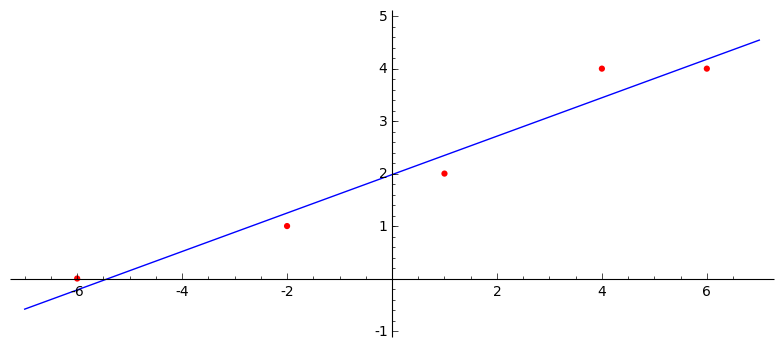
\includegraphics[scale=0.35]{figures/moindres_carres1}\quad
%    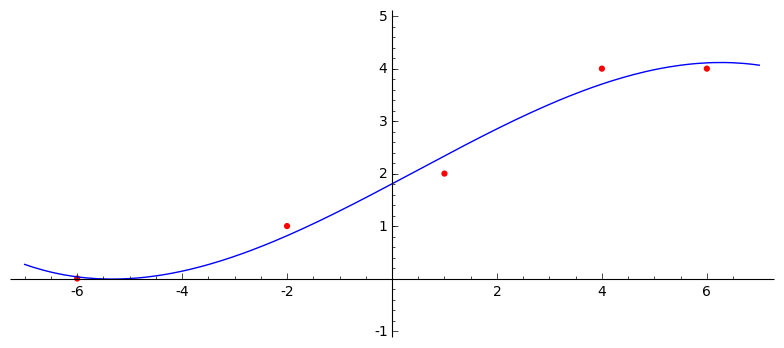
\includegraphics[scale=0.35]{figures/moindres_carres2}
%\end{center} 
%  
%\begin{enumerate}
%  \item Bien sûr les points ne sont pas alignés, donc il n'existe 
%  pas de droite passant par tous ces points.
%  On cherche une droite d'équation $y = a +bx$ qui minimise (le carré de) la distance
%  entre les points et la droite. Posons $f(x) = a + bx$.
%  
%  Alors pour nos $n$ points $(x_i,y_i)$ donnés, on voudrait $f(x_i)=y_i$. 
%  $$
%  \left\{ 
%  \begin{array}{rcl}
%  f(x_1) &=& y_1 \\
%  f(x_2) &=& y_2 \\
%  \vdots && \vdots\\
%  f(x_n) &=& y_n \\
%  \end{array}
%  \right.
%  \quad
%  \iff
%  \quad
%  \left\{ 
%  \begin{array}{rcl}
%  a +b x_1 &=& y_1 \\
%  a +b x_2 &=& y_2 \\
%  \vdots && \vdots\\
%  a +b x_n &=& y_n \\
%  \end{array}
%  \right.
%  \quad
%  \iff
%  \quad 
%  \begin{pmatrix}
%  1 & x_1 \\
%  1 & x_2 \\
%  \vdots & \vdots \\
%  1 & x_n \\  
%  \end{pmatrix}
%  \begin{pmatrix}
%  a \\ b  
%  \end{pmatrix}
%  = 
%  \begin{pmatrix}
%  y_1\\
%  y_2 \\
%  \vdots \\
%  y_n
%  \end{pmatrix}
%  \quad
%  \iff
%  \quad 
%  AX = B.
%  $$
%  
%  On résout (de façon non exacte) notre problème $AX = B$, par la formule des moindres carrés
%  $X = (A^TA)^{-1} A^T B$. Comme $X = \left(\begin{smallmatrix}a\\b\end{smallmatrix}\right)$,
%  on obtient l'équation $y=a+bxb$ de la droite des moindres carrés (voir la figure ci-dessus).
%  
%   La fonction \codeinline{moindres_carres} résout le problème général des moindres carrés.
%  Il reste ensuite à définir la matrice $A$ et le vecteur $B$ en fonction de notre liste de points
%  afin de trouver $X$.
%  Le code est le suivant :
%  \insertcode{algos/moindres_carres-tex1.sage}{moindres\_carres.sage (1)} 
%  
%
%  
%  \item L'idée est la même, mais cette fois les inconnues 
%  sont les coefficients de la fonction
%  $f(x) = a + bx +c x^2 + dx^3$ :
%   $$
%  \left\{ 
%  \begin{array}{rcl}
%  f(x_1) &=& y_1 \\
%  f(x_2) &=& y_2 \\
%  \vdots && \vdots\\
%  f(x_n) &=& y_n \\
%  \end{array}
%  \right.
%  \quad
%  \iff
%  \quad
%  \left\{ 
%  \begin{array}{rcl}
%  a +b x_1 + c x_1^2 + d x_1^3 &=& y_1 \\
%  a +b x_2 + c x_2^2 + d x_2^3 &=& y_2 \\
%  \vdots && \vdots\\
%  a +b x_n + c x_n^2 + d x_n^3 &=& y_n \\
%  \end{array}
%  \right.
%  $$
%  $$
%  \iff
%  \quad 
%  \begin{pmatrix}
%  1 & x_1 & x_1^2 & x_1^3\\
%  1 & x_2 & x_2^2 & x_2^3 \\
%  \vdots & \vdots & \vdots & \vdots\\
%  1 & x_n & x_n^2 & x_n^3  \\  
%  \end{pmatrix}
%  \begin{pmatrix}
%  a \\ b \\ c \\ d
%  \end{pmatrix}
%  = 
%  \begin{pmatrix}
%  y_1\\
%  y_2 \\
%  \vdots \\
%  y_n
%  \end{pmatrix}
%  \quad
%  \iff
%  \quad 
%  AX = B
%  $$ 
%  
%  Voici le code pour les mêmes points et une interpolation 
%  polynomiale de degré $d$ :
%  \insertcode{algos/moindres_carres-tex2.sage}{moindres\_carres.sage (2)} 
%    
%  
%\end{enumerate}
%
%Pour conclure, voici la preuve de la formule 
%(\ref{eq:moindrescarres}) des moindres carrés.
%Caractérisons géométriquement la condition << $\| AX -B \|$ minimale >>.
%On note $\Im A$ l'image de $A$, c'est-à-dire le sous-espace 
%vectoriel engendré par les vecteurs colonnes de la matrice $A$.
%Notons $p : \Rr^n \to \Rr^n$ la projection orthogonale sur $\Im A$.
%Enfin, notons $Y=p(B)$ le projeté orthogonal de $B$ sur l'image de $A$. 
%
%\myfigure{1.2}{  
%  \tikzinput{fig_formel_alglin_01}
%}
%
%Comme $Y$ est dans l'image de $A$ alors il existe $X$ tel que
%$AX=Y$ et $X$ est notre <<solution>> cherchée.
%En effet, c'est l'une des caractérisations du projeté orthogonal : 
%$Y = p(B)$ est le point de $\Im A$ qui minimise la distance entre $B$ et un 
%point de $\Im A$. 
%  
%  
%  Que $Y$ soit le projeté orthogonal de $B$ sur $\Im A$ signifie
%  que le vecteur $B-Y$ est orthogonal à tout vecteur de $\Im A$:
%  \begin{eqnarray*}
%    && \langle AV \mid B-Y \rangle = 0 \quad \forall V \in \Rr^p \\
%    & \iff & \langle AV \mid B-AX \rangle = 0 \quad \forall V \in \Rr^p \quad \text{ pour } Y=AX\\
%    & \iff & (AV)^T \cdot (B-AX)= 0 \quad \forall V \in \Rr^p \quad \text{ car } \langle u \mid v\rangle = u^T\cdot v\\
%    & \iff & V^T  A^T (B-AX)= 0 \quad \forall V \in \Rr^p \\    
%    & \iff & A^T (B-AX)= 0 \\
%    & \iff & A^TAX= A^T B \\
%    & \iff & X = (A^TA)^{-1} A^TB \\    
%  \end{eqnarray*} 
%
%%Remarque : nous admettons (et nous supposons) que la matrice $A^TA$ est inversible 
%%lorsque $A$ est de rang maximal (donc de rang $p$, car pour nous $p \le n$).
%


%%%%%%%%%%%%%%%%%%%%%%%%%%%%%%%%%%%%%%%%%%%%%%%%%%%%%%%%%%%%%%%%
\section{Courbes et surfaces}

La visualisation est une étape importante dans l'élaboration 
des preuves en mathématiques. L'avènement des logiciels de calcul 
formel possédant une interface graphique évoluée a 
rendu cette phase attrayante. Nous allons explorer 
les possibilités graphiques offertes par \Sage.
Nous avons déjà vu comment tracer les graphes de fonctions avec la commande \codeinline{plot}
(voir \og Premiers pas avec \Sage\ \fg{}), par exemple \codeinline{plot(sin(x)*exp(x),(x,-3,3))}
trace le graphe de la fonction $f(x)=\sin(x)\exp(x)$ sur l'intervalle $[-3,3]$.
\begin{center}
 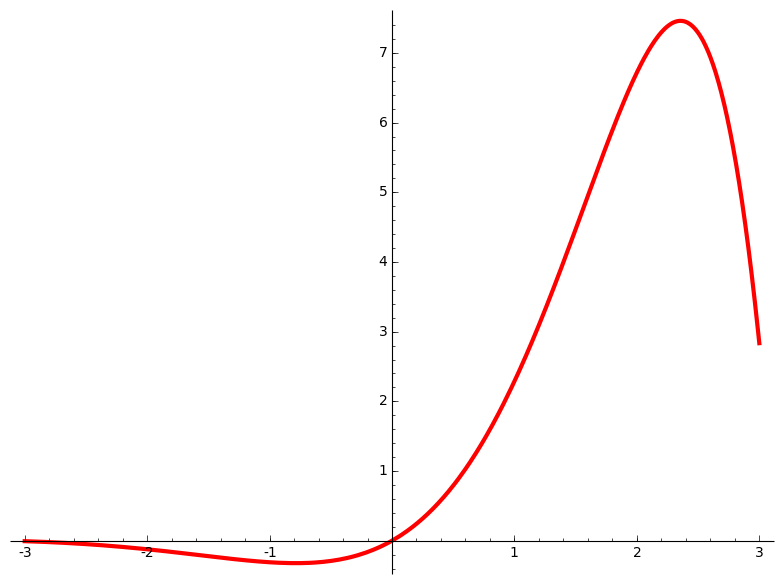
\includegraphics[scale=0.3]{figures/intro_courbes} 
\end{center}

En plus des graphes de fonctions \Sage\ sait tracer des courbes et des surfaces par d'autres méthodes.

%--------------------------------------------------------
\subsection{Courbes paramétrées}

La commande \codeinline{parametric_plot((f(t), g(t)), (t, a, b))} 
permet de tracer la courbe paramétrée plane donnée par les points 
de coordonnées $(f(t), g(t))$ lorsque le paramètre $t$ varie 
dans l'intervalle $[a,b]$. 
Commençons par la lemniscate de Bernoulli :


\begin{center}
 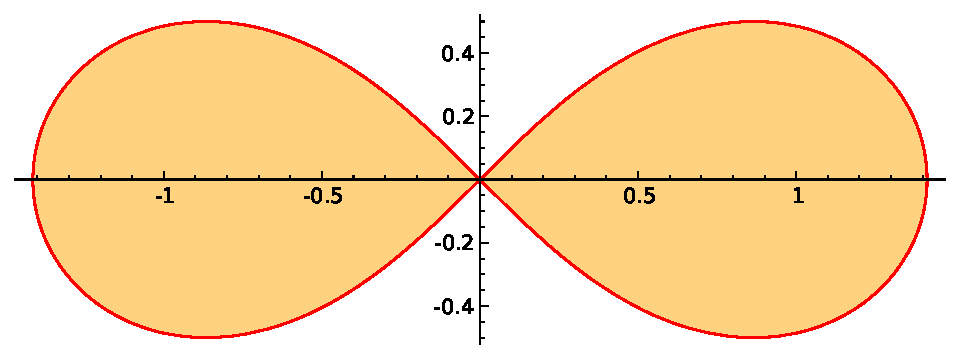
\includegraphics[scale=0.7]{figures/lemniscate_bernoulli} 
\end{center}




\insertcode{algos/lemniscate_bernoulli-tex.sage}{lemniscate-bernoulli.sage}


\begin{tp}
\sauteligne
\begin{enumerate}
  \item Tracer la spirale de Fermat d'équation
  $$\left\{
\begin{array}{l}
x(t)=\sqrt t \cos t\\[1mm]
y(t)=\sqrt t \sin t
\end{array}
\right. \qquad t \in \Rr_+.$$
  \item Tracer la courbe du papillon
  $$\left\{
\begin{array}{l}
x(t) = \sin(t)\left(\exp(\cos(t))-2\cos(4t)-\sin^5\left(\frac{t}{12}\right)\right)\\[3mm]
y(t) = \cos(t)\left(\exp(\cos(t))-2\cos(4t)-\sin^5\left(\frac{t}{12}\right)\right)
\end{array}
\right. \qquad t \in \Rr.$$
\end{enumerate} 
\end{tp}


\begin{center}

\includegraphics[scale=0.5]{figures/fermat_spiral}\quad
\includegraphics[scale=0.4]{figures/butterfly_curve}  
\end{center}


Les commandes de tracé possèdent de nombreuses options, 
qu'on pourra découvrir grâce 
à la commande \codeinline{help(parametric_plot)}. 
Par exemple :
\begin{itemize}
  \item Imposer un repère orthonormé : \codeinline{aspect_ratio = 1}

  \item Nombre de points pour le tracé : \codeinline{plot_points = 500}
    
  \item Ne pas afficher les axes : \codeinline{axes = False}
  
  \item Afficher une grille : \codeinline{gridlines = True}
  
  \item Remplir l'intérieur : \codeinline{fill = True}
  
  \item Couleur du trait : \codeinline{color = 'red'},
  couleur du remplissage : \codeinline{fillcolor = 'orange'}

\end{itemize}

% \insertcode{algos/fermat_spiral.sage}{fermat-spiral.sage}
% \insertcode{algos/butterfly_curve.sage}{butterfly-curve.sage}

%--------------------------------------------------------
\subsection{Courbes en coordonnées polaires}

Les courbes en coordonnées polaires sont tracées grâce à la 
commande \codeinline{polar_plot(r(t),(t,a,b))}, qui produira 
l'ensemble des points de coordonnées polaires $[r(t):t]$ pour 
$t$ variant dans l'intervalle $[a,b]$.
Voici le folium de Dürer d'équation 
$r(t) = \sin \frac t 2$, $t \in \Rr$.


\begin{center}
 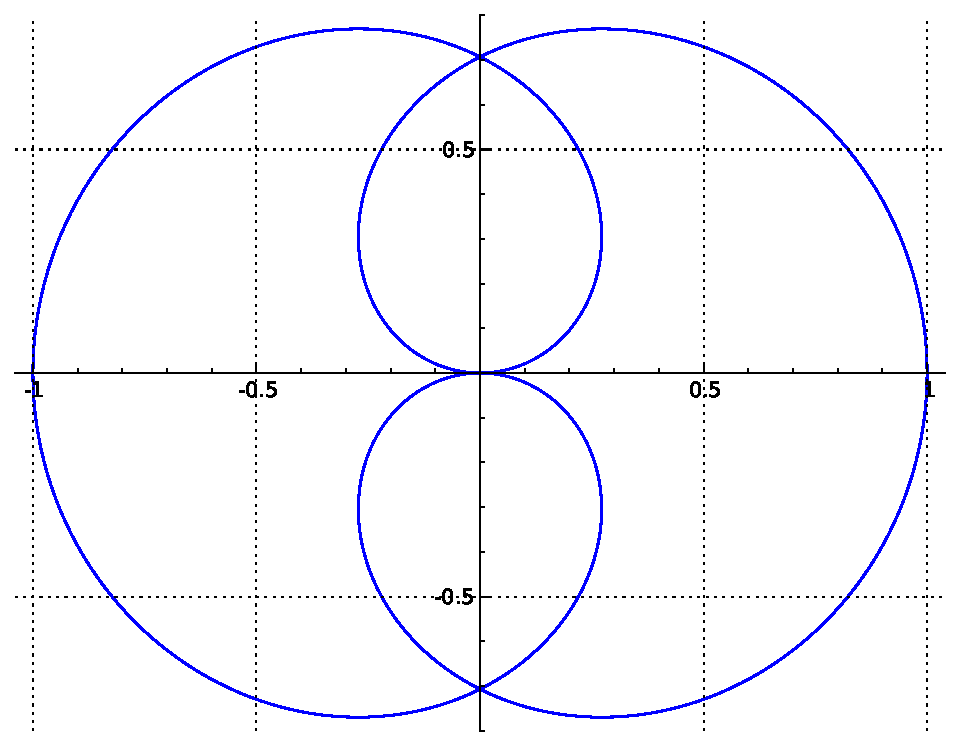
\includegraphics[scale=0.5]{figures/durer_folium} 
\end{center}


\insertcode{algos/durer_folium-tex.sage}{durer-folium.sage}

%Les options sont sensiblement les mêmes que celles 
% de la commande \codeinline{parametric_plot}, 
% on pourra y accéder grâce à la commande 
% \codeinline{help(polar_plot)}. 
% Voici quelques exemples.




\begin{tp}
\sauteligne
\begin{enumerate}
  \item Tracer la courbe du Lituus d'équation polaire 
  $$r(t)^2 = \frac{1}{t} \qquad t \in \Rr^*.$$
  \item Tracer la cochléoïde d'équation polaire 
  $$r(t) = \frac{\sin t}{t} \qquad t \in \Rr^*.$$
\end{enumerate} 
\end{tp}

Indications : on peut définir deux graphes \codeinline{G1}, 
\codeinline{G2} pour chacun des intervalles de définition. On superpose
les graphes avec \codeinline{G = G1 + G2}, puis on les affiche avec 
\codeinline{G.show()}.


\begin{center}
  \begin{minipage}{0.49\textwidth}
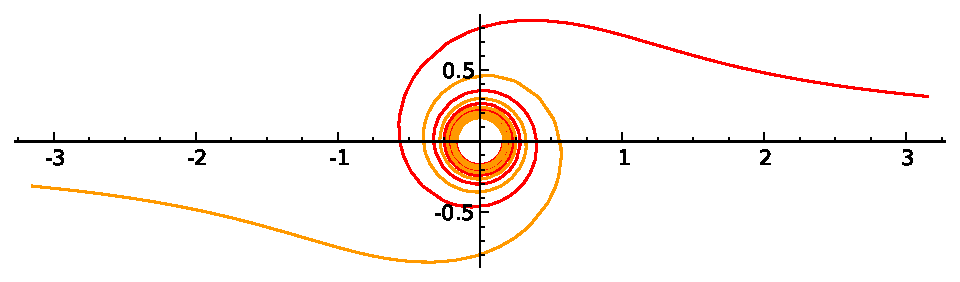
\includegraphics[scale=0.5]{figures/lituus}  
\end{minipage}
\begin{minipage}{0.49\textwidth}
\qquad\qquad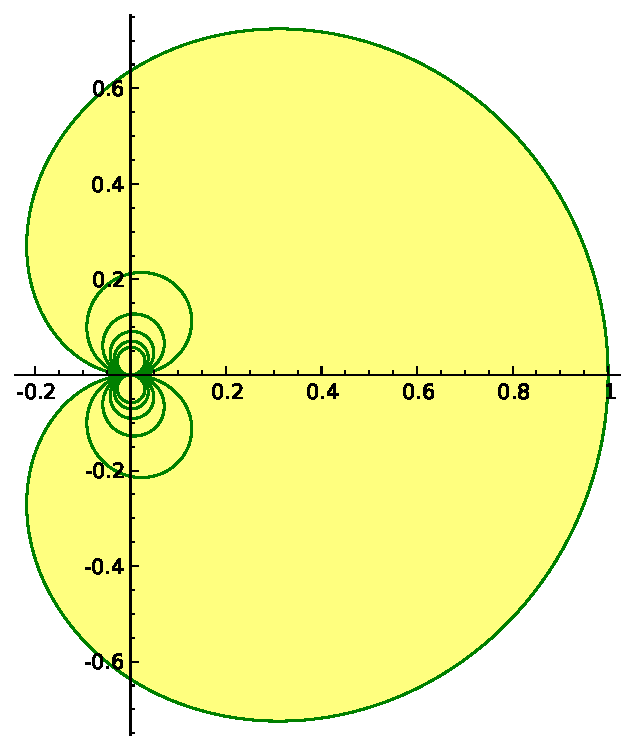
\includegraphics[scale=0.5]{figures/cochleoid}  
\end{minipage}
\end{center}



% \insertcode{algos/lituus.sage}{lituus.sage}
% \insertcode{algos/cochleoid.sage}{cochleoid.sage}



%--------------------------------------------------------
\subsection{Courbes définies par une équation}

Une courbe peut avoir plusieurs types de représentations, comme par exemple
un cercle d'équation paramétrique $(\cos t,\sin t)$ ou d'équation implicite
$x^2+y^2 = 1$.
La commande \\
\centerline{\codeinline{implicit_plot(f(x, y), (x, a, b), (y, c, d))} }
permet de tracer l'ensemble des couples $(x,y)$ 
dans $[a,b]\times[c,d]$ qui sont solutions de l'équation 
$f(x,y)=0$. Voici une autre courbe de papillon, cette fois algébrique. 

\insertcode{algos/butterfly_curve_algebraic-tex.sage}{butterfly-curve-algebraic.sage}


Noter comment il est possible de sauvegarder une image du tracé dans un fichier externe.


\begin{center}
  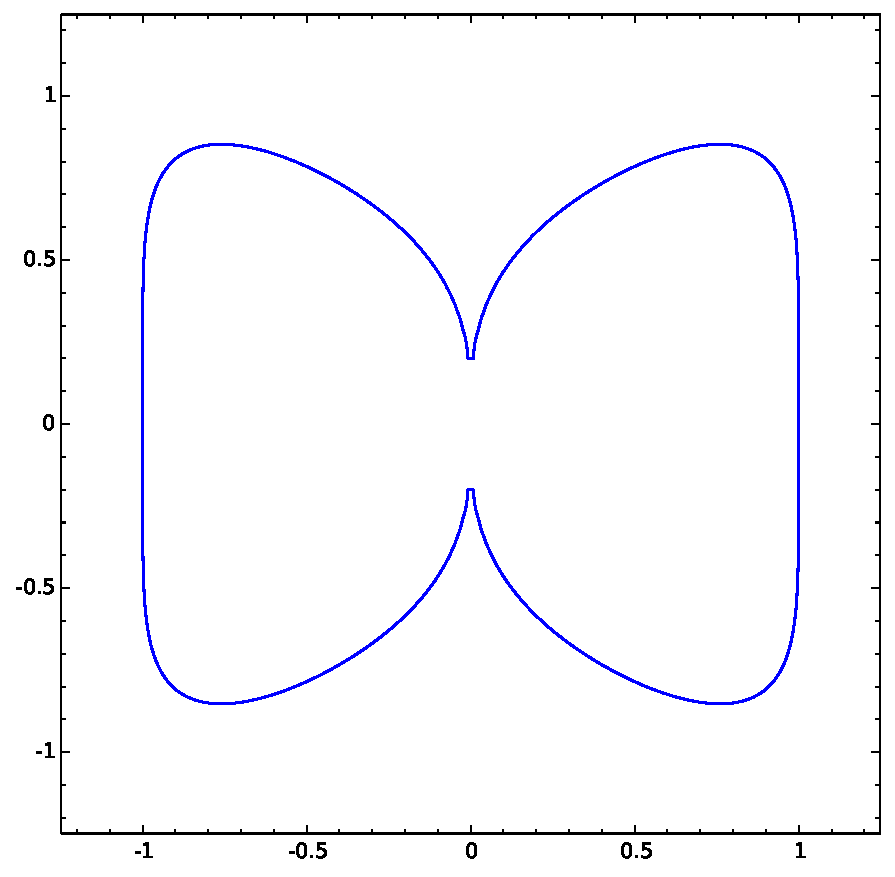
\includegraphics[scale=0.4]{figures/butterfly_curve_algebraic}
\end{center}

\begin{tp}
\sauteligne
\begin{enumerate}
  \item Définir une fonction qui renvoie la courbe définie par
  $$y^2-x^3+x+c = 0$$
  en fonction du paramètre $c\in \Rr$.
  \item \`A l'aide de la commande \codeinline{animate}, 
  réaliser une animation qui affiche l'évolution de la courbe
  pour $c \in[-1,1]$.
\end{enumerate}
\end{tp}


\begin{center}
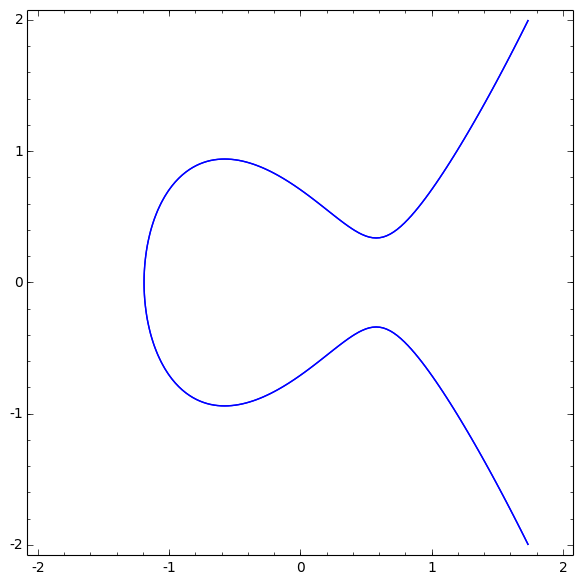
\includegraphics[scale=0.3]{figures/elliptic1}\quad
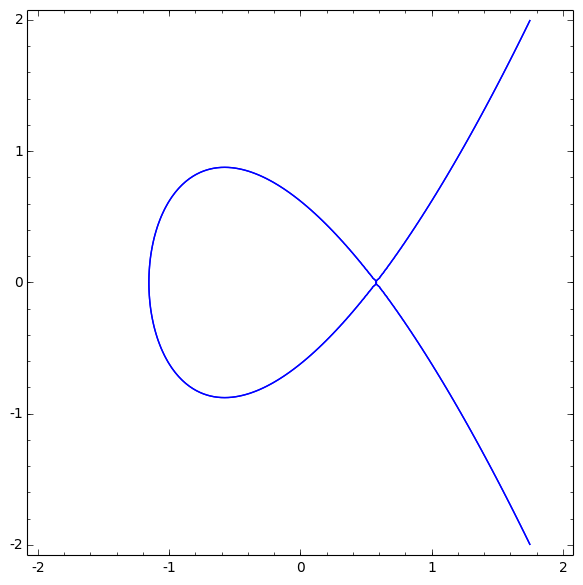
\includegraphics[scale=0.3]{figures/elliptic2}\quad
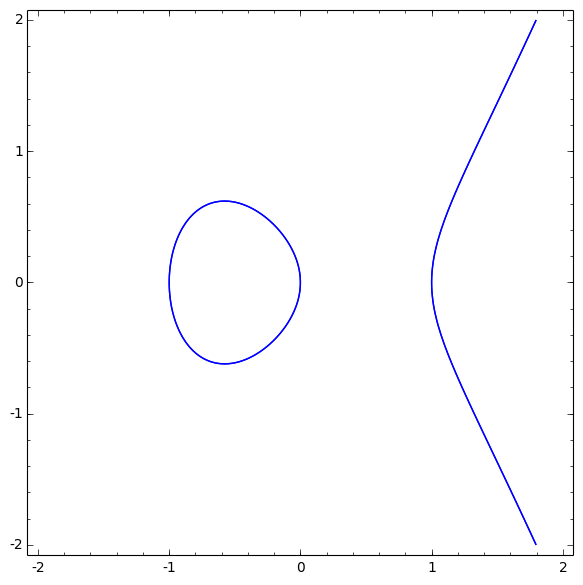
\includegraphics[scale=0.3]{figures/elliptic3}
\end{center}



%--------------------------------------------------------
\subsection{Courbes de l'espace}



La commande \codeinline{parametric_plot((x, y, z), (t, a, b))}, 
(ou bien \codeinline{parametric_plot3d()}) analogue à celle de la dimension $2$, 
trace la courbe paramétrée de 
l'espace donnée par les points de coordonnées $\big( x(t), y(t), z(t) \big)$ 
lorsque le paramètre $t$ varie dans l'intervalle $[a,b]$. 

\begin{tp}
Tracer la courbe d'Archytas d'équation paramétrique :
$$\left\{
\begin{array}{l}
x(t) = \cos^2 t \\[1mm]
y(t) = \cos t \sin t \\[1mm]
z(t) = \pm\sqrt{ \cos t(1-\cos t) }
\end{array}
\right.\qquad  t \in \big[-\tfrac\pi2,+\tfrac\pi2\big].$$
\end{tp}

%\insertcode{algos/archytas_curve.sage}{archytas-curve.sage}

Vous obtiendrez une figure qu'il est possible d'orienter dynamiquement 
avec la souris. Voici quelques-unes de ces vues.

\begin{center}
 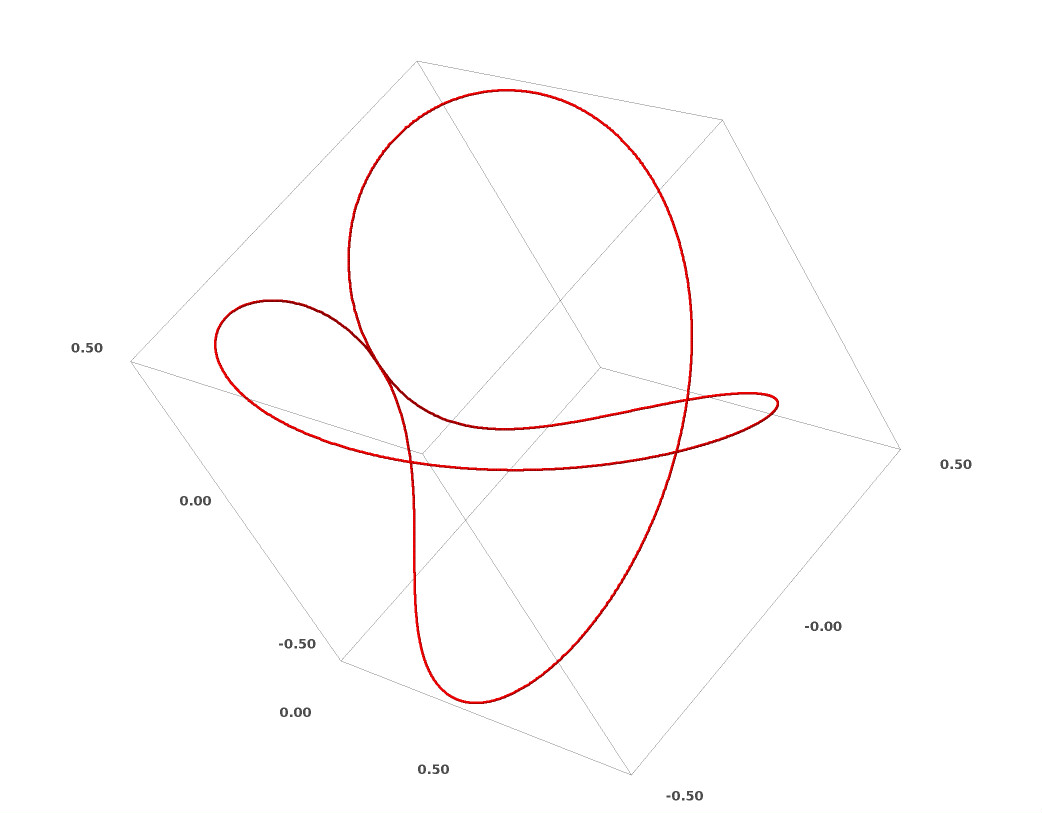
\includegraphics[scale=0.2]{figures/archytas_curve_new1.jpg} 
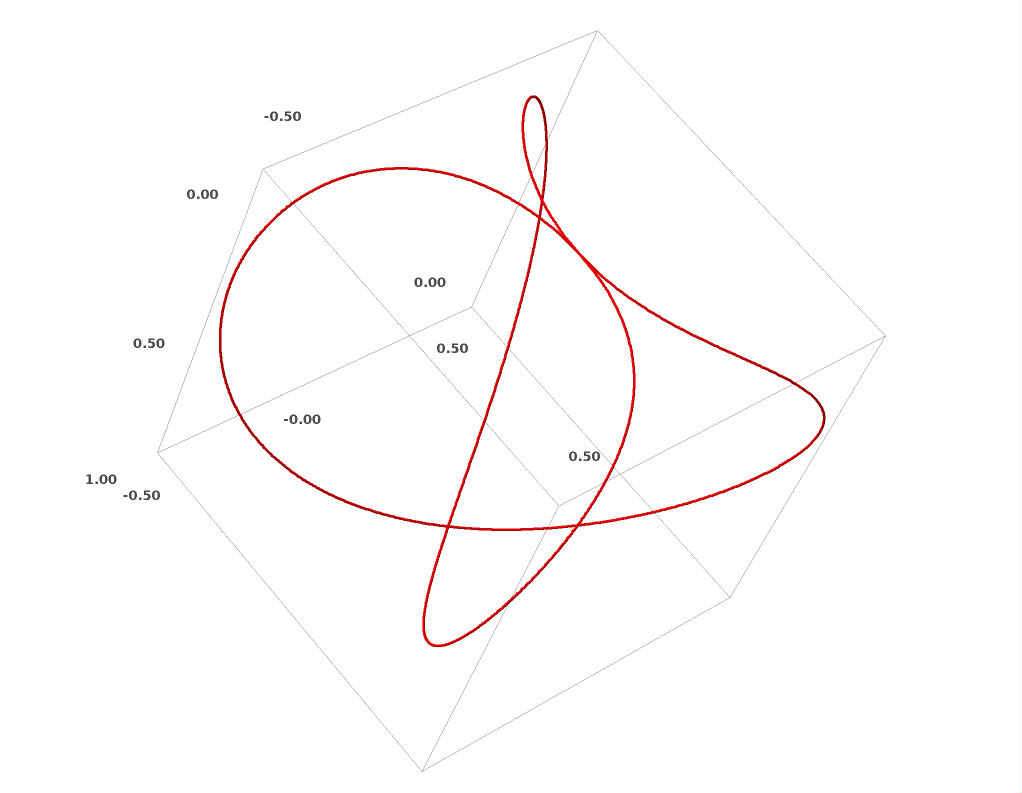
\includegraphics[scale=0.2]{figures/archytas_curve_new2.jpg}  
\end{center}




%--------------------------------------------------------
\subsection{Surfaces}


Découvrez, à l'aide de l'énoncé suivant, les différentes méthodes 
pour tracer des surfaces avec \Sage.

\begin{tp}
\sauteligne
\begin{enumerate}
  \item Tracer le graphe de la fonction $f(x,y)= x^2y^2-(x^2+y^2)^3$ définie
  sur $(x,y) \in [-1,1]\times[-1,1]$. Utiliser la fonction \codeinline{plot3d}.
  
  \item Tracer la surface d'Enneper
  définie par l'équation 
  $$\left( \frac{y^2-x^2}{2z}+\frac29z^2+\frac23\right)^3-
  6\left( \frac{y^2-x^2}{4z}-\frac14\big(x^2+y^2+\frac89z^2\big)+\frac29 \right)^2=0.$$
  Utiliser la fonction \codeinline{implicit_plot3d}.

  
  \item Tracer la nappe paramétrée définie par :
  $$\left\{
  \begin{array}{l}
  x(s,t) =  t^2 \cos s\\[1mm]
  y(s,t) =  s^2 \sin t\\[1mm]
  z(s,t) = \cos t+ \sin t
  \end{array}
  \right.\qquad  s \in \big[0,1\big], \quad t \in \big[-\pi,+\pi\big].$$
  Utiliser la fonction \codeinline{parametric_plot3d}.
  
  \item Tracer la surface paramétrée définie en coordonnées cylindriques par :
  $$r(\theta,z) = z^3 \cos \theta \qquad \theta \in [0,2\pi], \quad z \in [0,2].$$  
  Utiliser la fonction \codeinline{cylindrical_plot3d}.
  
  \item Tracer la surface paramétrée définie en coordonnées sphériques par 
  $$r(\theta,\phi)  = \theta \sin(2\phi) \qquad \theta \in [-1,2\pi], \quad  \phi \in [0,\pi].$$
  Utiliser la fonction \codeinline{spherical_plot3d}.  
\end{enumerate}
\end{tp}


%\insertcode{algos/surface.sage}{surface.sage}


\begin{center}
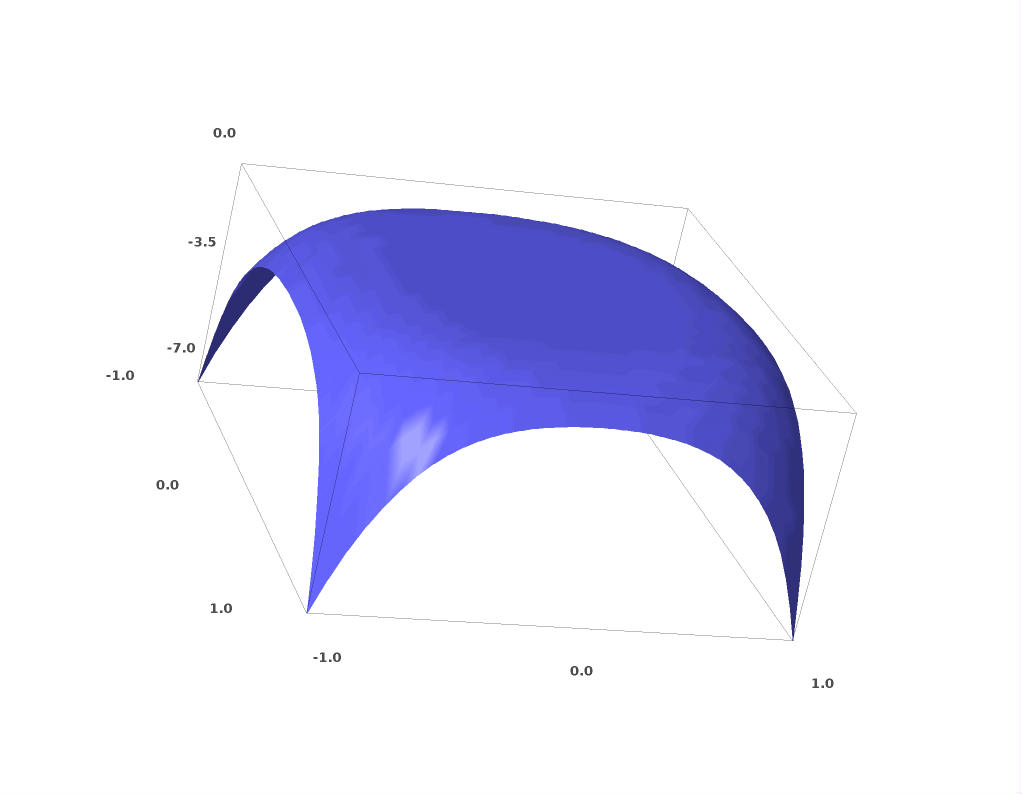
\includegraphics[scale=0.2]{figures/surface_1.jpg} 
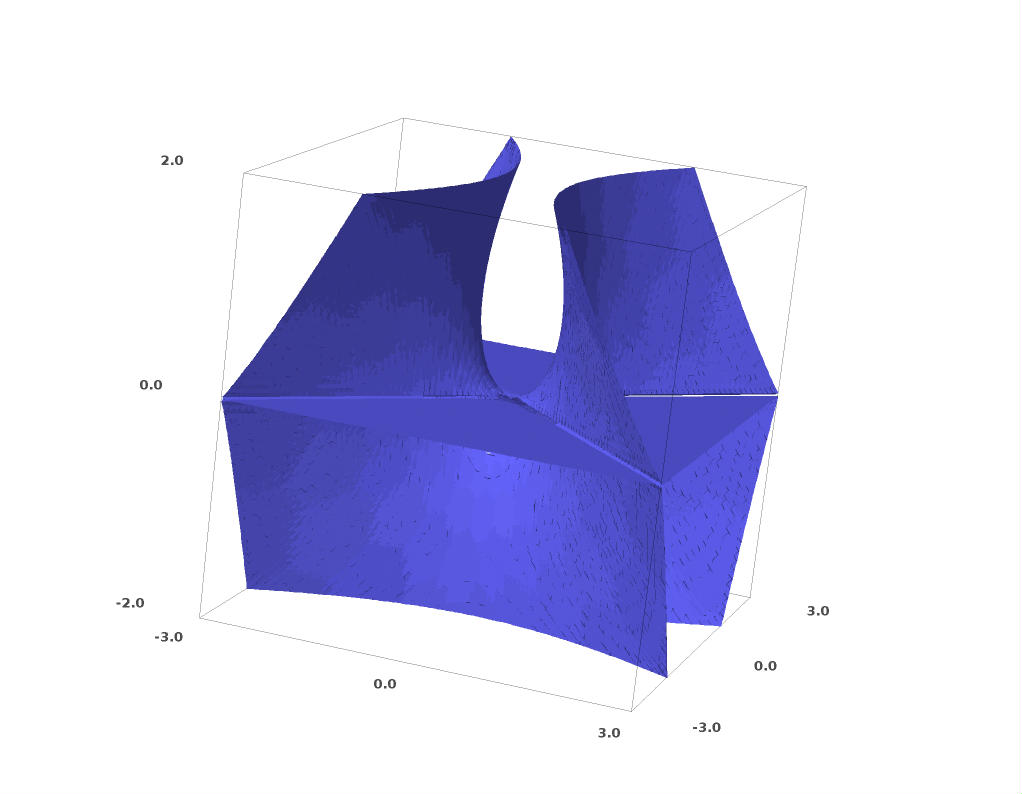
\includegraphics[scale=0.2]{figures/surface_2.jpg} \\ 
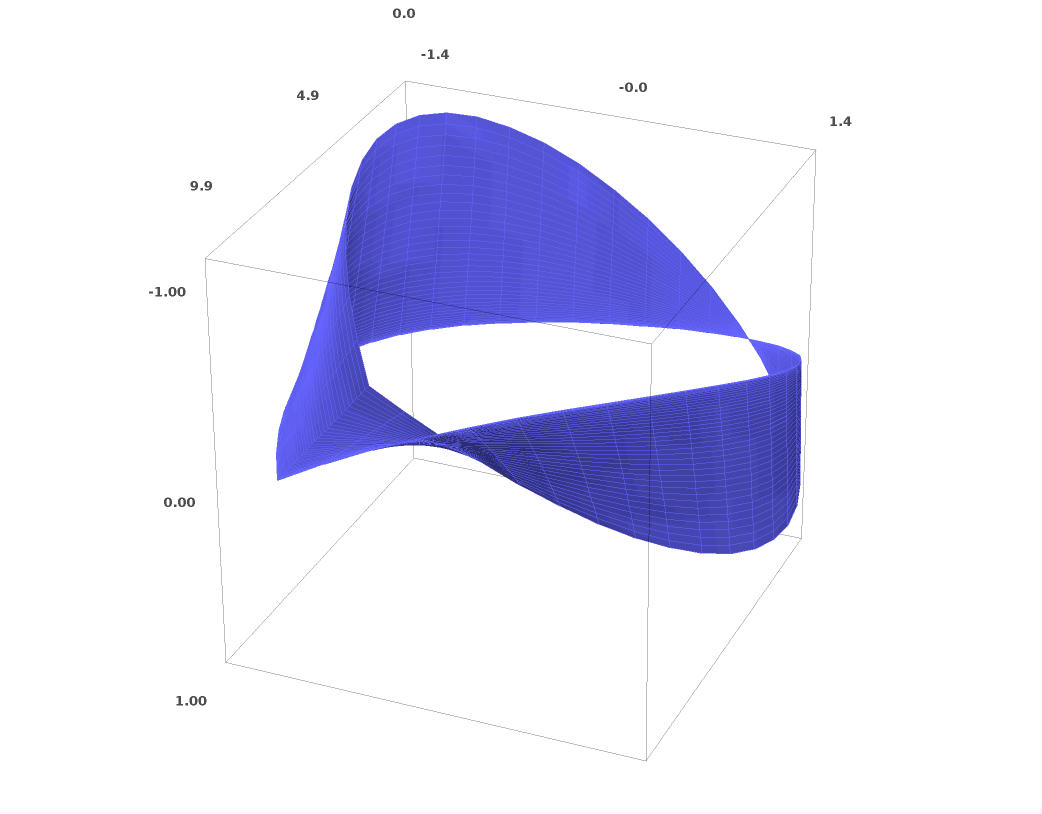
\includegraphics[scale=0.2]{figures/surface_3.jpg} \\
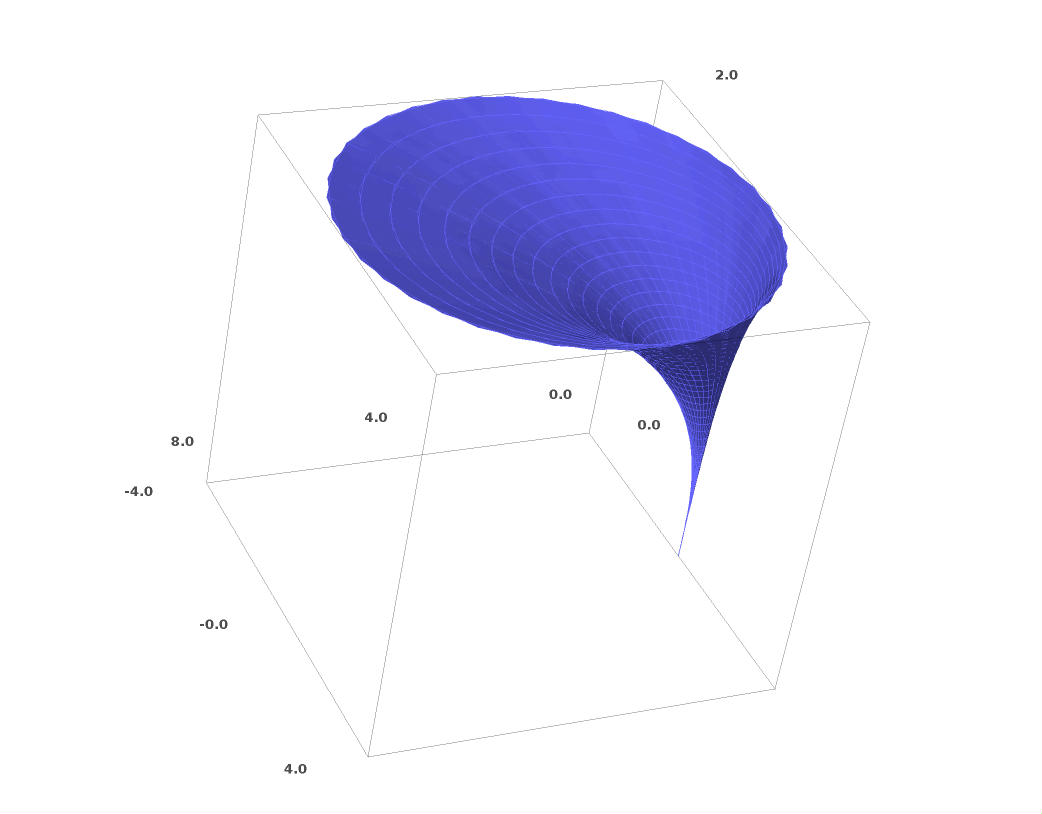
\includegraphics[scale=0.2]{figures/surface_4.jpg} 
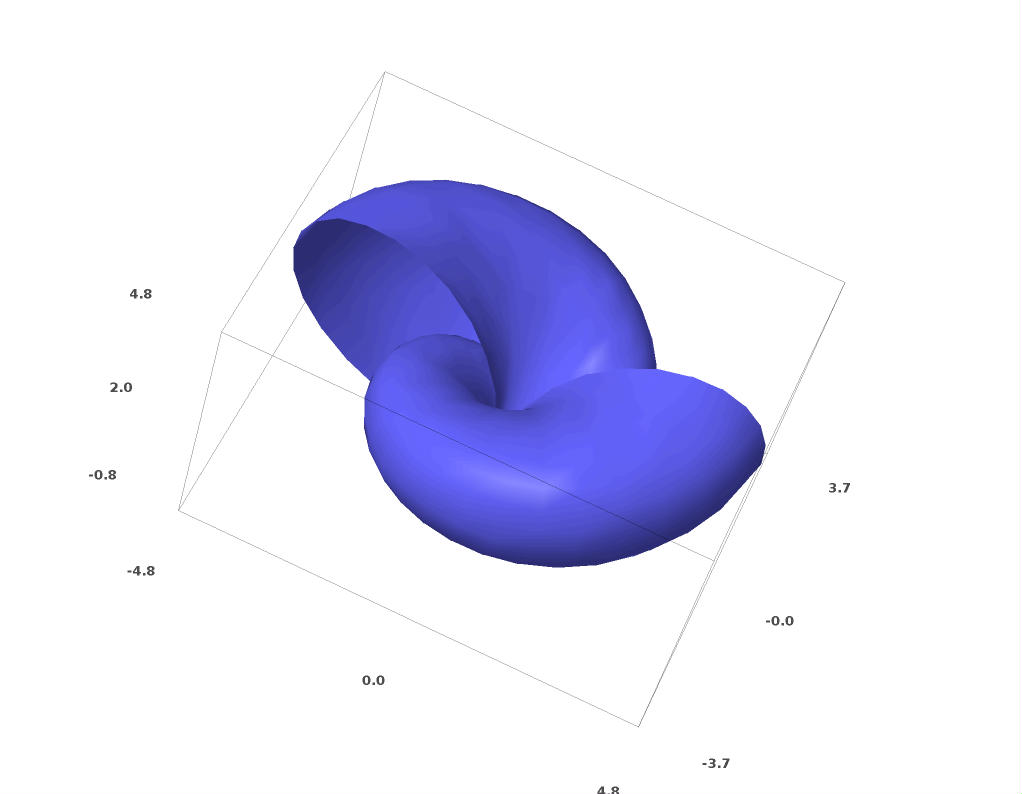
\includegraphics[scale=0.2]{figures/surface_5.jpg}  
\end{center}




%--------------------------------------------------------
\subsection{\'Etude d'une courbe paramétrée}

\begin{tp}
\'Etudier en détail la courbe paramétrée du plan définie par 
  $$\left\{
  \begin{array}{l}
  x(t) =  t^3-2t\\[1mm]
  y(t) =  t^2-t
  \end{array}
  \right.\qquad  t \in \Rr.$$
\begin{enumerate}
  \item Tracer la courbe.
  
  \item Trouver les points d'intersection de la courbe avec l'axe des ordonnées.
  
  \item Trouver les points en lesquels la tangente est verticale, puis horizontale.
  
  \item Trouver les coordonnées des points doubles.
\end{enumerate}
\end{tp}



\begin{center}
  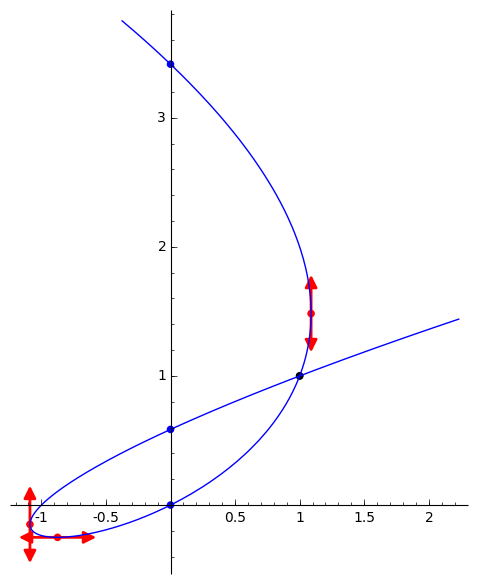
\includegraphics[scale=0.5]{figures/courbe.png} 
\end{center}



\begin{enumerate}
  \item La courbe a l'allure d'une boucle.
  \item On définit \codeinline{x = t^3-2*t} et \codeinline{y = t^2-t}.
On obtient les valeurs de $t$ correspondant aux points d'intersection de la courbe
avec l'axe $(x=0)$ en résolvant l'équation $x(t)=0$ : \codeinline{solve(x==0,t)}.
On obtient trois solutions $t \in \{-\sqrt2,0,+\sqrt2\}$ correspondant aux trois points
$\{(0,2+\sqrt2),(0,0),(0,2-\sqrt2)\}$
  
  \item On définit les fonctions dérivées $x'(t)$ et $y'(t)$
  par \codeinline{xx = diff(x,t)} et \codeinline{yy = diff(y,t)},
  les valeurs de $t$ pour lesquelles la tangente à la courbe est verticale s'obtiennent en résolvant
  l'équation $x'(t)=0$, ce qui s'écrit \codeinline{solve(xx==0,t)}.
  
  \item Trouver les points doubles est souvent un calcul délicat (même pour un logiciel de calcul formel).
  Il s'agit ici de résoudre le système d'équations polynomiales :
   $$\left\{
  \begin{array}{l}
  x(s) =  x(t)\\[1mm]
  y(s) =  y(t)
  \end{array}
  \right.\qquad  s,t \in \Rr.$$ 
  Mais il faut exclure la solution évidente $t=s$. Algébriquement cela signifie
  que $(s-t)$ divise les polynômes de deux variables $x(s)-x(t)$ et
  $y(s)-y(t)$. Autrement dit, il s'agit de résoudre :
   $$\left\{
  \begin{array}{l}
  \dfrac{x(s)-x(t)}{s-t} = 0  \\[1mm]
  \dfrac{y(s)-y(t)}{s-t} = 0
  \end{array}
  \right.\qquad  s,t \in \Rr.$$   
  Le code suivant fournit la solution 
  $(s,t) = \big(\frac{1-\sqrt5}{2}, \frac{1+\sqrt5}{2}\big)$, il y a un unique 
  point double ayant pour coordonnées $(1,1)$.
  \insertcode{algos/courbe-tex.sage}{courbe.sage} 
\end{enumerate}



%--------------------------------------------------------
\subsection{La projection stéréographique}

\begin{tp}
Soit $ \mathcal{S}$ la sphère centrée à l'origine de $\Rr^3$ et de rayon $1$.
On note $N = (0,0,1)$ le pôle Nord. Soit $\mathcal{P}$ le plan
équatorial d'équation $(z=0)$. La \defi{projection stéréographique}
est l'application $\Phi : \mathcal{S} \setminus \{N\} \to \mathcal{P}$
qui à un point $S$ de la sphère associe le point $P = (NS) \cap \mathcal{P}$
défini par l'intersection de la droite $(NS)$ avec le plan $\mathcal{P}$.

\begin{enumerate}
  \item En écrivant la relation $\vect{NP} = k \vect{NS}$ et sachant que $P \in \mathcal{P}$, trouver
  $k$ et en déduire $P$.
  
  Vérifier ainsi que l'application $\Phi$ est définie par :
  $$\Phi : \mathcal{S} \setminus \{N\} \to \mathcal{P} \qquad 
  \Phi(x,y,z) = \left( \frac{x}{1-z}, \frac{y}{1-z} \right)$$
  Définir la fonction correspondante avec \Sage.
  
  \item  Définir et vérifier que l'application inverse est :
  $$\Psi : \mathcal{P} \to \mathcal{S} \setminus \{N\} \qquad
  \Psi (X,Y) = \left( \frac{2X}{\rho},\frac{2Y}{\rho},1-\frac{2}{\rho}  \right) \quad \text{ avec } \rho = 1+X^2+Y^2$$
      
  \item \'Ecrire une fonction qui dessine une courbe paramétrée $\mathcal{C}'$ : $\big( x(t),y(t) \big)$, $t\in[a,b]$
  du plan $\mathcal{P}$, et qui dessine aussi l'image inverse de la courbe sur la sphère, $\mathcal{C} = 
  \Psi(\mathcal{C}')$.
 
  
  \item Vérifier graphiquement deux propriétés fondamentales de la projection stéréographique :
  \begin{enumerate}
    \item \og La projection stéréographique envoie les cercles de la sphère sur des cercles ou des droites du plan.\fg
    \item \og La projection stéréographique préserve les angles.\fg\ En particulier, deux courbes qui se coupent
    à angle droit, s'envoient sur deux courbes qui se coupent à angle droit.
  \end{enumerate}
  
  \item Soit $\mathcal{C}'$ la spirale logarithmique d'équation
  $\big( e^t \cos t, e^t \sin t \big)$, $t \in \Rr$.
  Tracer la loxodromie de la sphère qui est $\mathcal{C} = 
  \Psi(\mathcal{C}')$. 
  
  \item  Soit la courbe $\mathcal{C} \subset \mathcal{S}$
  définie par $\frac{1}{13t^2 - 6t + 2}\big(4t, -6t + 2, 13t^2 - 6t\big)$.
  Montrer que son image $\mathcal{C}' = \Phi(\mathcal{C}) \subset \mathcal{P}$
  est une droite, dont vous déterminerez une équation.
  
\end{enumerate}

\end{tp}

\begin{enumerate}
  \item ~
  

\begin{center}
  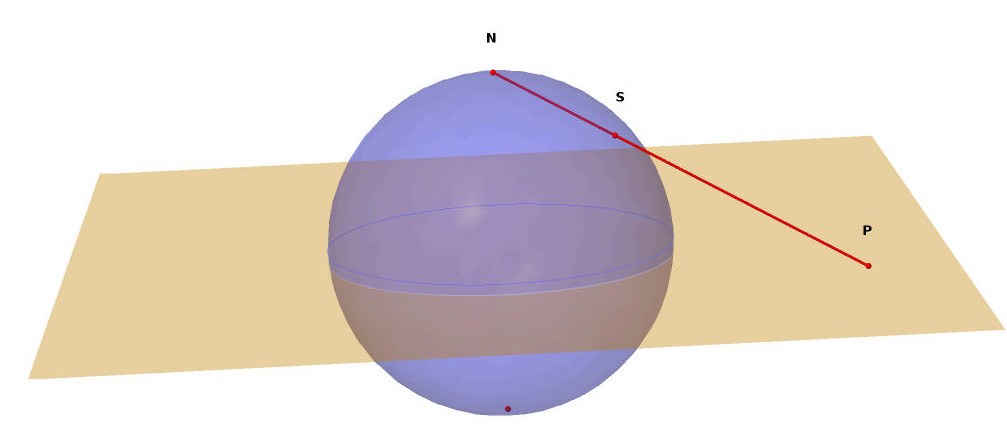
\includegraphics[scale=0.3]{figures/stereo1bis.jpg} 
\end{center}

  Le vecteur $\vect{NP}$ est colinéaire au vecteur $\vect{NS}$, donc il existe
  $k\in \Rr$ tel que  $\vect{NP} = k \vect{NS}$. Mais en plus on veut que
  $P \in \mathcal{P}$, c'est-à-dire $z_P = 0$. Ce qui permet de trouver $k$
  et d'en déduire $P = N + k\vect{NS}$. 
  On laisse \Sage\ faire les calculs :
 \insertcode{algos/stereographic-tex1.sage}{stereographic.sage (1)}
 
  On obtient $k = \frac{1}{1-z}$, et alors si $S=(x,y,z)$,
  $P = \left( \frac{x}{1-z}, \frac{y}{1-z}, 0 \right)$.
  En identifiant les points du plan à $\Rr^2$, on a ainsi prouvé 
  $\Phi(x,y,z) = \left( \frac{x}{1-z}, \frac{y}{1-z} \right)$.
  D'où la définition de la fonction $\Phi$ : 
\insertcode{algos/stereographic-tex2.sage}{stereographic.sage (2)}  

  \item Voici la fonction $\Psi$ :
\insertcode{algos/stereographic-tex3.sage}{stereographic.sage (3)}  
  
  On profite du fait que l'on nous donne le candidat, 
  pour se contenter de vérifier que c'est bien la bijection réciproque, c'est-à-dire
  $\Phi\big( \Psi(X,Y) \big) = (X,Y)$ pour tout $(X,Y) \in \Rr^2$.
  La composition s'écrit
\insertcode{algos/stereographic-tex4.sage}{stereographic.sage (4)}
 et comme on obtient \codeinline{newX = X} et \codeinline{newY = Y}, cela prouve le résultat.
 
 Il est possible de composer les fonctions de plusieurs variables, mais il faut rajouter
 une \og\codeinline{*}\fg\ devant la fonction à composer :\\
 \centerline{\codeinline{stereo(*inverse_stereo(X,Y)))}}
 cela renvoie \codeinline{X,Y} ce qui prouve bien 
  $\Phi\big( \Psi(X,Y) \big) = (X,Y)$.
  (L'opérateur \og\codeinline{*}\fg\ devant une liste permet de la décompacter, par exemple
  \codeinline{*(2,5,7)}  s'interprète comme \codeinline{2,5,7} qui peut alors être passé en argument à une fonction.)
  
  Pour prouver $\Psi\big( \Phi(x,y,z) \big) = (x,y,z)$, il faudrait se souvenir
  que $(x,y,z) \in \mathcal{S}$, donc $x^2+y^2+z^2=1$.
 
  \item  Voici comment tracer les courbes.
  La courbe du plan est tracée comme une ligne polygonale,
  avec un pas assez petit. Ensuite on calcule l'image par 
  $\Psi$ de chacun de ces points.
  
 \insertcode{algos/stereographic-tex5.sage}{stereographic.sage (5)} 
 
 Par exemple \codeinline{G = courbes(t^3,t^2,-2,2)}, trace la courbe
 du plan d'équation paramétrique $\big(t^3,t^2\big)$, $t\in[-2,2]$, ainsi
 que son image par la projection stéréographique inverse.
 
 Voici le cas d'un cercle et d'une droite du plan qui se coupent à angle droit,
 de même que les cercles de la sphères.
 

\begin{center}
  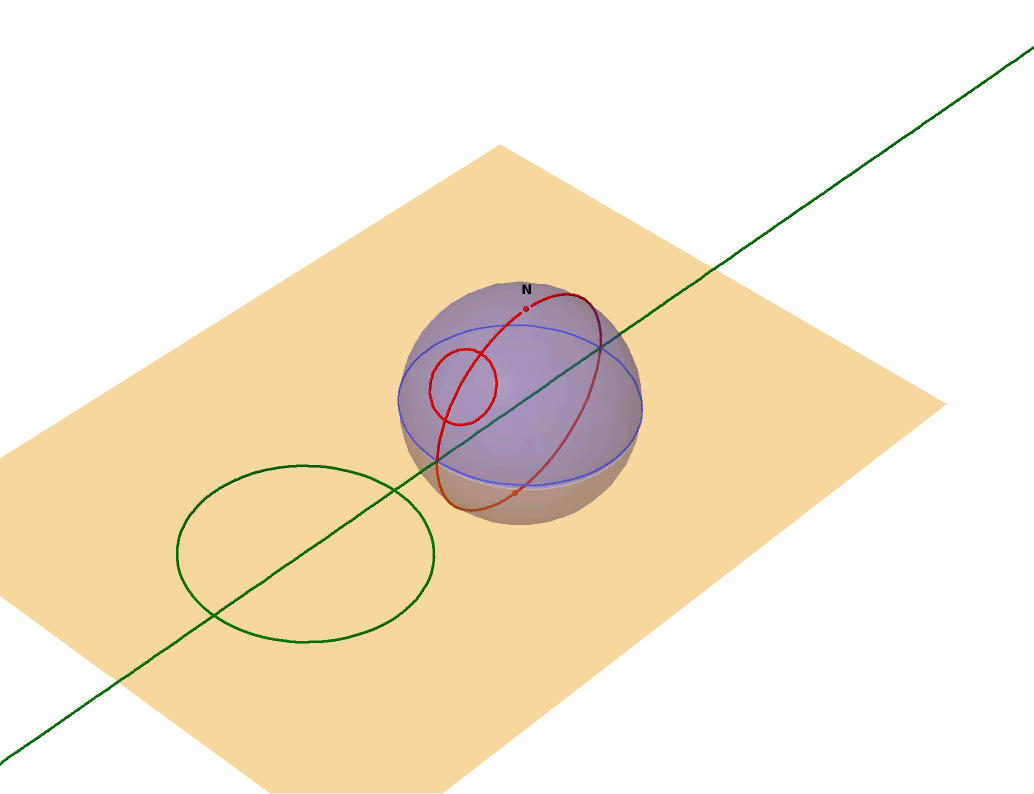
\includegraphics[scale=0.3]{figures/stereo2.jpg} 
\end{center}


  \item Voici une loxodromie de la sphère, courbe utilisée par les navigateurs, car elle
  correspond à une navigation à cap constant.
  

\begin{center}
  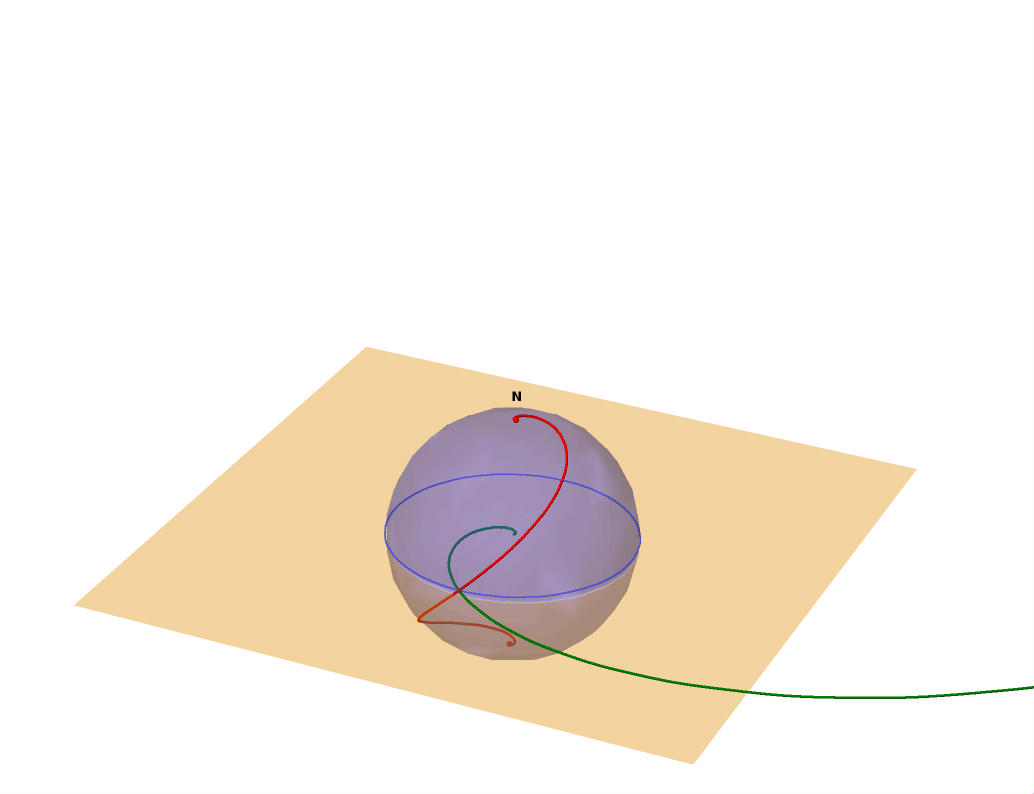
\includegraphics[scale=0.3]{figures/stereo3.jpg} 
\end{center}




  \item Pour $x,y,z$ définis par la paramétrisation, on calcule l'image par la projection stéréographique
  avec \codeinline{X,Y = stereo(x,y,z)}, on n'oublie pas de simplifier à l'aide de 
  \codeinline{full_simplify()}. Cela donne une paramétrisation de l'image,
  $x(t) = 2t$, $y(t) = -3t + 1$, qui est bien l'équation d'une droite.
  
\end{enumerate}



%%%%%%%%%%%%%%%%%%%%%%%%%%%%%%%%%%%%%%%%%%%%%%%%%%%%%%%%%%%%%%%%
\section{Calculs d'intégrales}

%--------------------------------------------------------
\subsection{\Sage\ comme une super-calculatrice}



\begin{tp}
Calculer à la main les primitives des fonctions suivantes. 
Vérifier vos résultats à l'ordinateur.
\begin{enumerate}
  \item $f_1(x) = x^4 + \frac{1}{x^2} + \exp(x)+ \cos(x)$
  \item $f_2(x) = x \sin(x^2)$ 
  \item $f_3(x) = \frac{\alpha}{\sqrt{1-x^2}} + \frac{\beta}{1+x^2} + \frac{\gamma}{1+x}$
  \item $f_4(x) = \frac{x^4}{x^2-1}$ 
  \item $f_5(x) = x^n \ln x$ pour tout $n\ge0$
\end{enumerate}
\end{tp}

Pour une fonction $f$, par exemple \codeinline{f(x) = x*sin(x^2)} donnée, la commande
\codeinline{integral(f(x),x)} renvoie une primitive de $f$.
Le résultat obtenu ici est \codeinline{-1/2*cos(x^2)}.

Quelques remarques :
\begin{itemize}
  \item La machine renvoie une primitive. Pour avoir l'ensemble des primitives, il faut
  bien entendu ajouter une constante.

  \item La fonction \codeinline{log} est la fonction logarithme népérien usuel, habituellement
  notée $\ln$.
  
  \item \codeinline{integral(1/x,x)} renvoie \codeinline{log(x)} alors
  que $\int \frac{\dd x}{x} = \ln |x|$. \Sage\ omet les valeurs absolues, ce qui ne l'empêche pas de faire
  des calculs exacts même pour les valeurs négatives. (En fait \Sage\ travaille avec le logarithme complexe.).
  
  \item Souvent, pour intégrer des fractions rationnelles, on commence par écrire 
  la décomposition en éléments simples. C'est possible avec
  la commande \codeinline{partial_fraction}. Par exemple pour
  \codeinline{f = x^4/(x^2-1)} la commande \codeinline{f.partial_fraction(x)} 
  renvoie la décomposition sur $\Qq$ : 
  $f(x) = x^2  + 1 - \frac12\frac{1}{x + 1} + \frac12\frac{1}{x - 1}$.
  
\end{itemize}



\begin{tp}
Calculer à la main et à l'ordinateur les intégrales suivantes.
\begin{enumerate}
  \item $\displaystyle I_1 = \int_1^3 x^2 + \sqrt{x} + \frac1x + \sqrt[3]{x} \; \dd x$
  \item $\displaystyle I_2 = \int_0^\frac{\pi}{2} \sin x (1+\cos x)^4 \; \dd x$
  \item $\displaystyle I_3 = \int_0^{\frac\pi6} \sin^3 x \; \dd x$
  \item $\displaystyle I_4 = \int_0^{\sqrt3} \frac{3x^3 - 2x^2 - 5x - 6}{(x + 1)^2(x^2 + 1)} \; \dd x$
\end{enumerate}
\end{tp}

Par exemple \codeinline{integral(sin(x)^3,x,0,pi/6)} renvoie 
$\frac23 - \frac{3\sqrt{3}}{8}$.



%--------------------------------------------------------
\subsection{Intégration par parties}

\begin{tp}
Pour chaque $n\ge 0$, nous allons déterminer une primitive de la fonction 
$$f_n(x) = x^n \exp(x).$$

\begin{enumerate}
  \item \Sage\ connaît-il directement la formule ?
  
  \item Calculer une primitive $F_n$ de $f_n$ pour les premières valeurs de $n$.
  
  \item 
  \begin{enumerate}
    \item \'Emettre une conjecture reliant $F_n$ et $F_{n-1}$.
    \item Prouver cette conjecture.
    \item En déduire une fonction récursive qui calcule $F_n$.
  \end{enumerate}
  
  \item 
  \begin{enumerate}
    \item \'Emettre une conjecture pour une formule directe de $F_n$.
    \item Prouver cette conjecture.
    \item En déduire une expression qui calcule $F_n$.
  \end{enumerate}  
\end{enumerate} 
\end{tp}

\begin{enumerate}
  \item La commande \codeinline{integral(x^n*exp(x),x)}
  renvoie le résultat \codeinline{(-1)^n*gamma(n + 1, -x)}. 
  Nous ne sommes pas tellement avancés ! \Sage\ renvoie une \emph{fonction spéciale} $\Gamma$ 
  que l'on ne connaît pas.  
  En plus (à l'heure actuelle, pour la version 6.6), dériver la primitive avec \Sage\ ne 
  redonne pas la même expression que $f_n$.
  
  \item Par contre, il n'y a aucun problème pour calculer les primitives $F_n$ 
  pour les premières valeurs de $n$. On obtient :
  $$\begin{array}{rcl}
    F_0(x) &=& \exp(x) \\
    F_1(x) &=& (x - 1)\exp(x) \\
    F_2(x) &=& (x^2 - 2x + 2)\exp(x) \\
    F_3(x) &=& (x^3 - 3x^2 + 6x - 6)\exp(x) \\
    F_4(x) &=& (x^4 - 4x^3 + 12x^2 - 24x + 24)\exp(x) \\
    F_5(x) &=& (x^5 - 5x^4 + 20x^3 - 60x^2 + 120x - 120)\exp(x) \\
  \end{array}$$  
   
    
  \item
  \begin{enumerate}
    \item Au vu des premiers termes, on conjecture $F_n(x) = x^n \exp(x) - nF_{n-1}(x)$.
    On vérifie facilement sur les premiers termes que cette conjecture est vraie.
    
    \Sage\ ne sait pas (encore) vérifier formellement cette identité 
    (avec $n$ une variable formelle). La commande suivante échoue à trouver $0$  : \\
    \centerline{\codeinline{integral(x^n*exp(x),x) - x^n*exp(x) + n*integral(x^(n-1)*exp(x),x)}}
    
    \item Nous prouverons la validité de cette formule en faisant 
    une intégration par parties
    (on pose par exemple $u=x^n$, $v'=\exp(x)$ et donc $u'=nx^{n-1}$, $v = \exp(x)$) :
    
    $$F_n(x) 
    = \int x^n \exp(x)\; \dd x 
    = \big[x^n\exp(x)\big] - \int nx^{n-1}\exp(x)\; \dd x
    = x^n\exp(x) - n F_{n-1}(x).$$
    
    \item Voici l'algorithme récursif pour le calcul de $F_n$ utilisant 
    la relation de récurrence.
    
    \insertcode{algos/integrales-ipp-tex1.sage}{integrales-ipp (1)}
    
  \end{enumerate} 
  
  \item Avec un peu de réflexion, on conjecture la formule 
  $$F_n(x) = \exp x \sum_{k=0}^n (-1)^{n-k} \frac{n!}{k!} x^k$$
  où $\frac{n!}{k!} =  n(n-1)(n-2)\cdots (k+1)$.
  
  Pour la preuve, on pose $G_n(x) = \exp(x)\sum_{k=0}^n (-1)^{n-k} \frac{n!}{k!} x^k$.
  On a 
  $$G_n(x) = \exp(x)\sum_{k=0}^{n-1} (-1)^{n-k} \frac{n!}{k!} x^k  + \exp(x)x^n
  = n G_{n-1}(x)+ \exp(x)x^n.$$ 
  Ainsi 
  $G_n$ vérifie la même relation de récurrence que $F_n$.
  De plus $G_0(x)=\exp x = F_0(x)$. Donc pour tout $n$, $G_n=F_n$.
  
  On peut donc ainsi calculer directement notre intégrale par la formule : \\  
  \centerline{\codeinline{exp(x)*sum((-1)^(n-k)*x^k*factorial(n)/factorial(k),k,0,n)}}
 
\end{enumerate}



%--------------------------------------------------------
\subsection{Changement de variable}

Soit $f$ une fonction définie sur un intervalle $I$ et $\varphi : J \to I$ 
une bijection de classe $\mathcal{C}^1$.
La formule de changement de variable pour les primitives est :
$$\int f(x) \; \dd x = \int f\big(\varphi(u)\big)\cdot\varphi'(u) \; \dd u.$$

La formule de changement de variable pour les intégrales, pour tout $a,b\in I$, est :
$$\int_a^b f(x) \; \dd x 
= \int_{\varphi^{-1}(a)}^{\varphi^{-1}(b)} f\big(\varphi(u)\big)\cdot\varphi'(u) \; \dd u.$$

\begin{tp}
\sauteligne
\begin{enumerate}
  \item Calcul de la primitive $\displaystyle\int \sqrt{1-x^2} \; \dd x$.
  \begin{enumerate}
    \item Poser $f(x) = \sqrt{1-x^2}$ et le changement de variable $x = \sin u$, c'est-à-dire on pose 
    $\varphi(u) = \sin u$.
    \item Calculer $f\big( \varphi(u) \big)$ et $\varphi'(u)$.
    \item Calculer la primitive de $g(u) = f\big(\varphi(u)\big)\cdot\varphi'(u)$.
    \item En déduire une primitive de $f(x) = \sqrt{1-x^2}$.
  \end{enumerate}
  
  \item Calcul de la primitive $\displaystyle\int \frac{\dd x}{1+\left(\frac{x+1}{x}\right)^{1/3}}$.
  \begin{enumerate}  
    \item Poser le changement de variable défini par l'équation $u^3 = \frac{x+1}{x}$.
    
    \item En déduire le changement de variable $\varphi(u)$ et $\varphi^{-1}(x)$.
  \end{enumerate}
  
  
  \item \'Ecrire une fonction \codeinline{integrale_chgtvar(f,eqn)} qui calcule
  une primitive de $f(x)$ par le changement de variable défini par l'équation 
  \codeinline{eqn} reliant $u$ et $x$.
  
  En déduire $\displaystyle\int (\cos x + 1)^n \cdot \sin x \; \dd x$, en posant $u= \cos x + 1$.
  
  \item Même travail avec \codeinline{integrale_chgtvar_bornes(f,a,b,eqn)}
  qui calcule l'intégrale de $f(x)$ entre $a$ et $b$ par changement de variable.
  
  En déduire $\displaystyle\int_0^{\frac\pi4} \frac{\dd x}{2+\sin^2 x}$, en posant $u = \tan x$.
\end{enumerate}
\end{tp}


\begin{enumerate}
  \item 
  \begin{enumerate}
    \item La fonction est $f(x) = \sqrt{1-x^2}$ et 
    on pose la fonction $\varphi(u) = \sin u$, c'est-à-dire que l'on 
    espère que le changement de variable $x = \sin u$ va simplifier le calcul de l'intégrale :
    
    \centerline{\codeinline{f = sqrt(1-x^2)} \qquad \codeinline{phi = sin(u)}}
    
    \item 
    On obtient $f\big( \varphi(u) \big)$ en substituant la variable $x$ par $\sin u$ :
    cela donne $f\big( \varphi(u) \big) = \sqrt{1-\sin^2 u} = \sqrt{\cos^2 u} = |\cos u|$.
    Ce qui s'obtient par la commande \codeinline{frondphi = f(x=phi)} (puis en simplifiant).    
    (Notez que \Sage\ \og oublie \fg{} les valeurs absolues, car il calcule en fait la 
    racine carrée complexe et pas réelle.
    Ce sera heureusement sans conséquence pour la suite.
    En effet pour que $f(x)$ soit définie, il faut $x \in [-1,1]$, comme $x = \sin u$
    alors $u \in [-\frac\pi2,\frac\pi2]$ et donc $\cos u \ge 0$.)    
    Enfin $\varphi'(u) = \cos u$ s'obtient par \codeinline{dphi = diff(phi,u)}.
    
    \item On pose $g(u) = f\big(\varphi(u)\big)\cdot\varphi'(u) = \cos^2 u = \frac{1+\cos(2u)}{2}$.
    Donc $\int g(u)\; \dd u = \frac{u}{2} + \frac{\sin(2u)}{4}$.
    
    \item Pour obtenir une primitive de $f$, on utilise la formule de changement de variable :
    $$\int \sqrt{1-x^2} \; \dd x = \int f(x)\; \dd x = \int g(u) \; \dd u =  \frac{u}{2} + \frac{\sin(2u)}{4}.$$
    Mais il ne faut pas oublier de revenir à la variable $x$,
    Comme $x = \sin u$ alors $u = \arcsin x$, donc 
    $$\int \sqrt{1-x^2} \; \dd x = \frac{\arcsin x}{2} + \frac{\sin(2\arcsin x)}{4}.$$
    
    Les commandes sont donc \codeinline{G = integral(g,u)} puis
    \codeinline{F = G(u = arcsin(x))} donne la primitive recherchée.
    Après simplification de $\sin(2\arcsin x)$, on obtient :
    $$\int \sqrt{1-x^2} \; \dd x = \frac{\arcsin x}{2} + \frac x2 \sqrt{1-x^2}.$$
    
  \end{enumerate}
  
  \item Pour calculer la primitive $\int \frac{\dd x}{1+\left(\frac{x+1}{x}\right)^{1/3}}$, l'énoncé
    nous recommande le changement de variable $u^3 = \frac{x+1}{x}$.
  La seule difficulté supplémentaire est qu'il faut exprimer $x$ en fonction de $u$
  et aussi $u$ en fonction de $x$.
  Pour cela on définit l'équation \codeinline{u^3 == (x+1)/x} reliant $u$ et $x$ : 
  \codeinline{eqn = u^3 == (x+1)/x}. On peut maintenant résoudre l'équation afin d'obtenir
  $\phi(u)$ ($x$ en fonction de $u$) :  \codeinline{phi = solve(eqn,x)[0].rhs()} et $\phi^{-1}(x)$ ($u$ en fonction de $x$) : \codeinline{phi_inv = solve(eqn,u)[0].rhs()}.
  Le reste se déroule comme précédemment.
 
  
  \item On automatise la méthode précédente :
  \insertcode{algos/integrales-chgtvar-tex1.sage}{integrales-chgtvar (1)}
  Ce qui s'utilise ainsi :
  \insertcode{algos/integrales-chgtvar-tex3.sage}{integrales-chgtvar (2)} 
  Et montre que 
  $$\int (\cos x + 1)^n \cdot \sin x \; \dd x =  -\frac{1}{n + 1}(\cos x + 1)^{n + 1}.$$
 
  \item Pour la formule de changement de variable des intégrales, on adapte la procédure précédente
  en calculant l'intégrale $\int_{\varphi^{-1}(a)}^{\varphi^{-1}(b)} g(u) \; \dd u$.
  
  Pour cela on calcule 
  $\varphi^{-1}(a)$ (par  \codeinline{a_inv = phi_inv(x=a)}) et 
  $\varphi^{-1}(b)$ (par  \codeinline{b_inv = phi_inv(x=b)}).
 
  Pour calculer $\int_0^{\frac\pi4} \frac{\dd x}{2+\sin^2 x}$,
  on pose  $u = \tan x$.
  Donc $x = \phi(u) = \arctan u$ et $u = \varphi^{-1}(x) = \tan x$.
  Nous avons $\phi'(u)= \frac{1}{1+u^2}$. D'autre part,
  comme $a=0$ alors $\varphi^{-1}(a) = \tan 0 = 0$
  et comme $b = \frac\pi4$ alors $\varphi^{-1}(b) = \tan \frac\pi4 = 1$.
  Ainsi la formule de changement de variable :
  $$\int_a^b f(x) \;\dd x =
  \int_{\varphi^{-1}(a)}^{\varphi^{-1}(b)} f\big(\varphi(u)\big)\cdot\varphi'(u) \; \dd u$$
  devient 
  $$I = \int_0^{\frac\pi4} \frac{1}{2+\sin^2 x} \; \dd x = 
  \int_0^1 \frac{1}{2+\sin^2 (\arctan u)} \frac{1}{1+u^2}  \; \dd u.$$
  Mais $\sin^2(\arctan u ) = \frac{u^2}{1+u^2}$ donc
  $$I = \int_0^1 \frac{1}{2+\frac{u^2}{1+u^2}} \frac{1}{1+u^2}  \; \dd u
  = \int_0^1 \frac{\dd u}{2+3u^2}  \; \dd u = \left[\frac{1}{\sqrt6}\arctan\left(\frac{\sqrt6}{2}\right)\right]_0^1
  = \frac{1}{\sqrt6}\arctan\left(\frac{\sqrt6}{2}\right).$$
  Ce que l'ordinateur confirme !
\end{enumerate}
%
%%%%%%%%%%%%%%%%%%%%%%%%%%%%%%%%%%%%%%%%%%%%%%%%%%%%%%%%%%%%%%%%%
%\section{Polynômes}
%
%%--------------------------------------------------------
%\subsection{Manipuler les polynômes}
%
%\begin{tp}
%Soient  $P(X) = X^4-3X^2-1$, $Q(X) = (X+1)^4$ des polynômes de $\Qq[X]$.
%Après avoir déclaré l'anneau des polynômes $\Qq[X]$ par \codeinline{R.<X> = QQ[]} 
%(où \codeinline{QQ} désigne le corps des rationnels), répondre aux questions suivantes :
%\begin{enumerate}
%  \item Est-ce que $\deg(P \cdot Q) = \deg P + \deg Q$ ?
%  \item Est-ce que $\deg(P - Q) = \max( \deg P, \deg Q )$ ?
%  \item Développer $Q$. Quel est le coefficient devant $X^3$ ?
%  \item Quel est le quotient de la division euclidienne de $P$ par $(X+1)^2$ ?
%  Et le reste ?
%  \item Quelles sont les racines de $Q$ ? Et celles de $P$ ?
%\end{enumerate}
%\end{tp}
%
%\begin{enumerate}
%  \item (et 2.) La commande \codeinline{degree()} permet d'obtenir le degré ; ainsi, 
%  après avoir déclaré l'anneau de polynômes $\Qq[X]$ et avoir défini les deux polynômes 
%  $P$ et $Q$, on teste les égalités sur les degrés.
%  
%\insertcode{algos/intro-polynome-tex1.sage}{intro-polynome.sage (1)} 
%
%  La première égalité est vraie, par contre la seconde est fausse (il n'y a pas toujours égalité des degrés).
%  Les énoncés vrais en toute généralité pour des polynômes non nuls sont :
%  $$\deg(P \cdot Q) = \deg P + \deg Q \quad\text{ et }\quad \deg(P + Q) \le \max( \deg P, \deg Q )$$
%
%  \setcounter{enumi}{2}
%  \item On développe un polynôme par \codeinline{expand(Q)}.
%  On récupère les coefficients comme si le polynôme était une liste :
%  \codeinline{Q[k]} renvoie le coefficient $a_k$ devant $X^k$.
%  
%  \item On obtient le quotient et le reste comme avec les entiers.
%  Le quotient \codeinline{P // (X+1)^2} vaut $X^2 - 2X$. 
%  Le reste \codeinline{P \% (X+1)^2} vaut $2X - 1$.
%  
%  \item La question est ambigüe ! Il faut préciser dans quel ensemble on cherche les racines.
%  Est-ce dans $\Qq$, $\Rr$ ou $\Cc$ ? Souhaitons-nous une racine exacte ou approchée ?
%  \begin{itemize}
%    \item \codeinline{P.roots()} : renvoie les racines du corps de base (ici $\Qq$). 
%    Renvoie ici une liste vide car $P$ n'a pas de racines rationnelles.
%    \item \codeinline{Q.roots()} renvoie \codeinline{[(-1, 4)]} car $-1$ est une racine de multiplicité $4$.
%    \item \codeinline{P.roots(QQbar)} : racines exactes dans $\Cc$ (pour un polynôme à coefficients dans $\Qq$).
%    Ici renvoie deux racines réelles et deux racines imaginaires pures :
%    \codeinline{-1.817354021023971?},
%    \codeinline{1.817354021023971?}, 
%    \codeinline{-0.5502505227003375?*I},
%    \codeinline{0.5502505227003375?*I}. 
%    Le point d'interrogation en fin d'écriture signifie que \Sage\ calcule avec les valeurs exactes, 
%    mais n'affiche que les premières décimales.
%    \item \codeinline{P.roots(RR)} : racines réelles \emph{approchées} :
%    \codeinline{-1.81735402102397}, \codeinline{1.81735402102397}. On quitte donc la résolution formelle
%    pour une résolution numérique approchée.
%    \item \codeinline{P.roots(CC)} : racines complexes \emph{approchées}.        
%  \end{itemize}
%\end{enumerate}
%
%
%
%\begin{tp}
%\sauteligne
%\begin{itemize}
%  \item Pour un polynôme $P \in \Cc[X]$ et un réel $r>0$, tracer l'image par $P$ du cercle 
%centré à l'origine de $\Cc$ et de rayon $r$.
%  
%  \item Faites varier $r$ (ou mieux faites une animation). 
%  En quoi cela illustre-t-il le théorème de d'Alembert-Gauss ?
%
%  
%  \item Application à $P(X) = X^4-X^3+X^2-\ii X+1 \in \Cc[X]$.
%\end{itemize}
%\end{tp}
%
%Voici quelques images de l'animation pour des valeurs de $r$ valant
%successivement : $r_0 = 0.5$, $r_1 = 0.6176\ldots$,
%$r_2 = 0.9534\ldots$, $r_3 = 1.2082\ldots$, $r_4 = 1.4055\ldots$ et $r_5 = 1.5$.
%\begin{center}
%  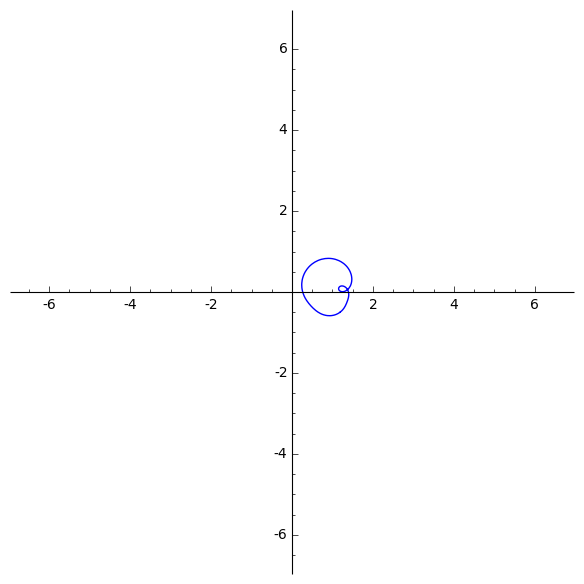
\includegraphics[scale=0.3]{figures/polynome1}\quad
%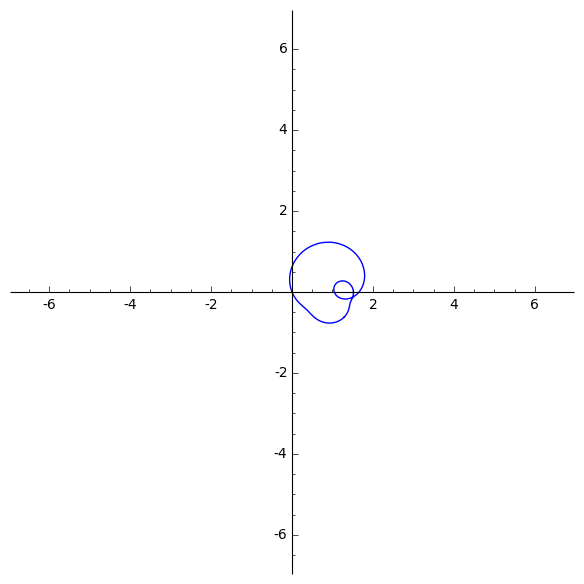
\includegraphics[scale=0.3]{figures/polynome2}\quad
%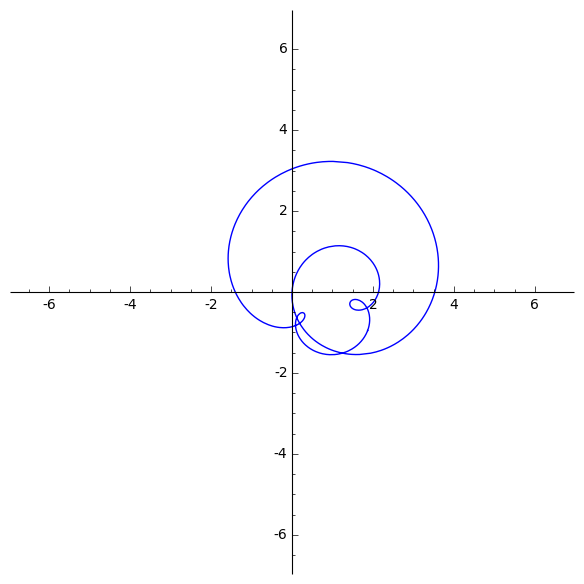
\includegraphics[scale=0.3]{figures/polynome3}
%\end{center}
%\begin{center}
%  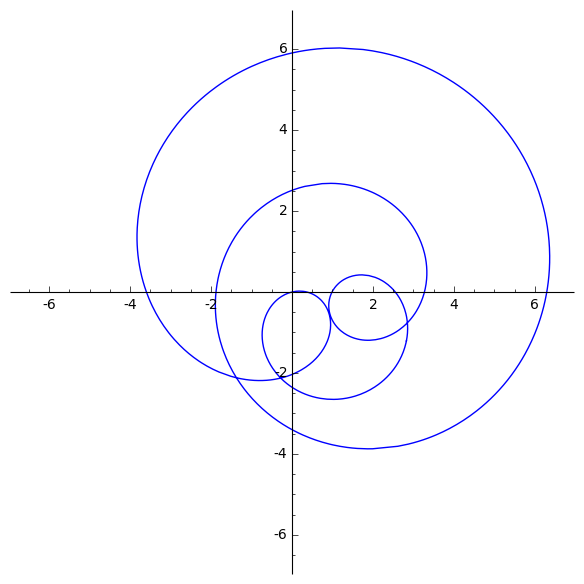
\includegraphics[scale=0.3]{figures/polynome4}\quad
%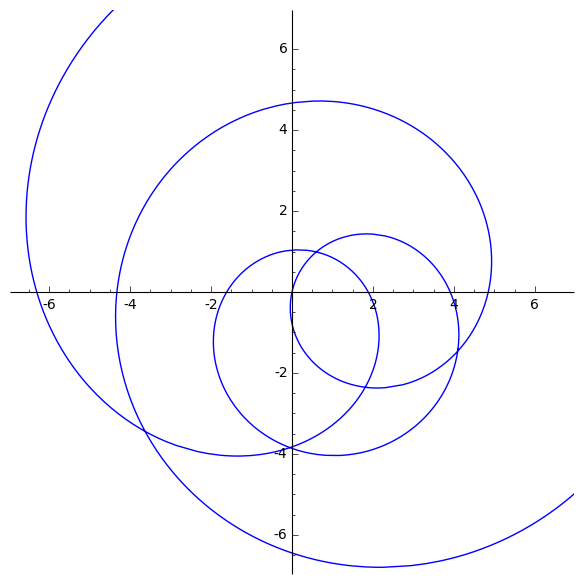
\includegraphics[scale=0.3]{figures/polynome5}\quad
%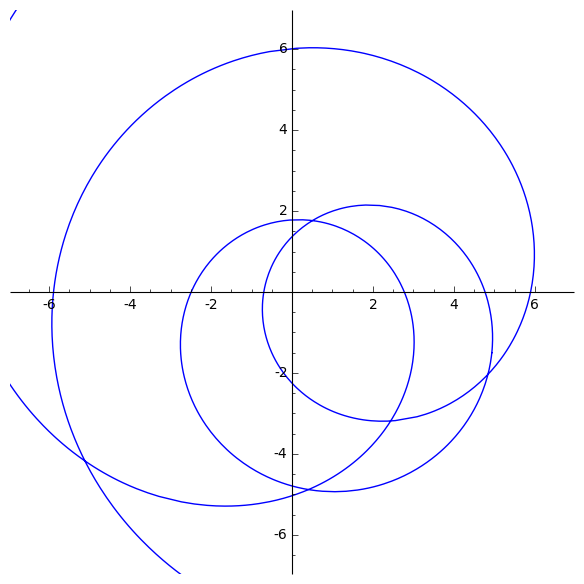
\includegraphics[scale=0.3]{figures/polynome6}
%\end{center}
%
%Quand la courbe $\mathcal{C}_r$ passe-t-elle par l'origine ? La courbe passe par l'origine
%s'il existe un nombre complexe $re^{\ii t}$ tel que $P(re^{\ii t}) = 0$ autrement dit lorsque 
%$P$ admet une racine de module $r$. D'après le théorème de d'Alembert-Gauss un polynôme de degré $n$ a au plus
%$n$ racines. Alors il y a au plus $n$ valeurs $r_1,\ldots,r_n$ pour lesquelles 
%$\mathcal{C}_{r_i}$ passe par l'origine.
%Pour notre exemple de degré $4$, il y a $4$ racines, qui conduisent ici à $4$ modules distincts,
%$r_1,\ldots,r_4$.
%
%\medskip
%
%Voici comment procéder :
%\begin{itemize}
%  \item On commence par définir l'anneau $\Cc[X]$ par \codeinline{R.<X> = CC[]}.
%  Les calculs seront donc des calculs approchés avec des nombres complexes.
%  Notre polynôme $P$ est défini par \codeinline{P = X^4-X^3+X^2-I*X+1}.
%  
%  \item 
%  Le cercle de rayon $r$ est l'ensemble des complexes de la forme $re^{\ii t}$ pour $t\in [0,2\pi]$.
%  La courbe $\mathcal{C}_r$ cherchée est donc l'ensemble 
%  $$\mathcal{C}_r = \big\{ P(re^{\ii t}) \mid t \in  [0,2\pi] \big\}.$$
%  
%  Voici la fonction qui renvoie ce tracé :
%\insertcode{algos/intro-polynome-tex2.sage}{intro-polynome.sage (2)}   
%  
%  \item Une animation est une juxtaposition d'images. 
%  On la définit par :\\  
%  \centerline{\codeinline{A = animate( [plot_image_cercle(P,r) for r in srange(0.5,1.5,0.05)] )}}  
%  puis on l'affiche par \codeinline{A.show()}.
%\end{itemize}
%
%\begin{remarque*}
%Par défaut \Sage\ fait les calculs dans un ensemble appelé \codeinline{SR} (\emph{Symbolic Ring}).
%Dans cet ensemble vous pouvez définir des expressions polynomiales et en trouver les racines.
%L'accès aux fonctions spécifiques aux polynômes (comme le degré, les coefficients,...) est un peu différent. Voici comment déclarer un polynôme, récupérer son degré ainsi que le coefficient devant $X^2$ :
% \insertcode{algos/intro-polynome-tex3.sage}{intro-polynome.sage (3)} 
%\end{remarque*}
%
%
%%--------------------------------------------------------
%\subsection{Algorithme de Horner}
%
%L'algorithme de Horner permet d'évaluer rapidement un polynôme $P$ en une valeur $\alpha$.
%Voyons comment il fonctionne à la main avec l'exemple de $P(X) = X^5 + X^4 - 5X^3 - 3X - 2$
%et $\alpha = 2$.
%
%Sur la première ligne du tableau, on écrit les coefficients de $P$, $a_n,a_{n-1},\ldots,a_1,a_0$.
%On reporte en troisième ligne première colonne, $a_n$, le coefficient dominant de $P$.
%On multiplie ce nombre par $\alpha$, on l'écrit en deuxième ligne, deuxième colonne, 
%% (sur la deuxième ligne, décalé d'un cran à droite),
%puis on ajoute $a_{n-1}$ que l'on écrit en troisième ligne, deuxième colonne.
%% (sur la troisième ligne juste en dessous). 
%Et on recommence. À chaque étape, on multiplie le dernier nombre obtenu par $\alpha$ et on lui ajoute un coefficient de $P$. 
%Le dernier nombre obtenu est $P(\alpha)$.
%
%\myfigure{1}{
%\tikzinput{fig_formel_polynome01}
%}
%
%Ici le dernier nombre est $0$, donc $P(2)=0$. Conclusion : $2$ est racine de $P$.
%
%
%Avec le même polynôme et $\alpha=-1$ le tableau se complète ainsi :
%\myfigure{1}{
%\tikzinput{fig_formel_polynome02}
%}
%
%ce qui implique $P(-1)=6$.
%
%Le travail à faire suivant formalise cette procédure et montre que l'algorithme de Horner permet des calculs efficaces avec les polynômes.
%
%\begin{tp}
%On fixe un corps $K$, et $\alpha\in K$. Soit $P(X) = a_nX^n+a_{n-1}X^{n-1}+\cdots +a_kX^k+\cdots+ a_1X+a_0 \in K[X]$.
%%Fixons $\alpha \in K$. 
%
%%Faire les applications avec 
%On pourra prendre pour les applications 
%$P(X) = X^5 + X^4 - 5X^3 - 3X - 2$ et $\alpha = 2$, puis $\alpha = -1$.
%
%\begin{enumerate}
%  \item Compter et comparer le nombre de multiplications nécessaires dans $K$ pour calculer 
%  $P(\alpha)$, par :
%  \begin{enumerate}
%    \item le calcul direct :
%    $$P(\alpha) = a_n \alpha^n+a_{n-1} \alpha^{n-1}+\cdots +a_k \alpha^k+\cdots+ a_1 \alpha +a_0,$$
%    
%    \item l'algorithme de Horner :
%    $$P(\alpha) =  \Big(\big((a_n \alpha+a_{n-1})\alpha +a_{n-2} \big) \alpha + \cdots +a_1\Big) \alpha +a_0.$$
%    
%    \item \'Ecrire une fonction qui calcule $P(\alpha)$ par l'algorithme de Horner.
%  \end{enumerate}
%  
%  \item On formalise le calcul précédent en définissant la suite :
%  $$b_{n} = a_n \qquad \text{ puis pour } \qquad n-1\ge k \ge 0\  : \ b_{k} = \alpha b_{k+1}  + a_k.$$
%  
%  \begin{enumerate}
%     
%    \item Montrer que dans la division euclidienne de $P(X)$ par $X-\alpha$ qui s'écrit :
%    $$P(X) = (X-\alpha) Q(X) + P(\alpha) $$
%    le reste $P(\alpha)$ est égal à $b_0$ et le quotient $Q(X)$ est égal au polynôme 
%    $b_{n}X^{n-1}+\cdots +b_2X+b_1$ 
%    %est constitué des 
%    dont les coefficients sont les $b_k$ pour $k\geq 1$.
%    
%    \emph{Indications.} Pour ce faire développer $(X-\alpha)Q(X)$ et retrouver 
%    pour les coefficients de $Q$ la même relation de récurrence que celle 
%    définissant la suite des $b_k$.
%
%  
%   \item Modifier votre fonction afin qu'elle calcule la suite $(b_{n},b_{n-1},\ldots,b_1,b_0)$
%   et qu'elle renvoie le quotient $Q$ et le reste $b_0 = P(\alpha)$.
%  
%  \item \'Ecrire une fonction qui calcule l'expression d'un polynôme $P(X)$ dans la base
%  des $(X-\alpha)^k$, c'est-à-dire calculer les $c_k \in K$ tels que :
%  $$P(X) = c_n (X-\alpha)^n+ c_{n-1}(X-\alpha)^{n-1}+ \cdots + c_1(X-\alpha) + c_0.$$
%  \end{enumerate}
%\end{enumerate}
%
%\end{tp}
%
%
%
%
%\begin{enumerate}
%  \item 
%  \begin{enumerate}
%    \item Le calcul d'un monôme $a_k\cdot \alpha^k$ de degré $k$ nécessite $k$ multiplications, donc pour calculer
%    $P(\alpha)$ il faut $n+(n-1)+\cdots+k+\cdots+1+0 = \frac{n(n+1)}{2}$ multiplications (et $n$ additions).
%    
%    \item La méthode de Horner 
%    $$P(\alpha) =  \Big(\big((a_n \alpha+a_{n-1})\alpha +a_{n-2} \big) \alpha + \cdots + a_1\Big) \alpha +a_0.$$
%    nécessite seulement $n$ multiplications (et $n$ additions). 
%    On passe d'un coût d'ordre $\frac12n^2$ à un coût d'ordre $n$ ; le gain est donc énorme.
%     
%    \item Pour l'implémentation, on note que la formule de récurrence 
%    se fait pour des indices $k$ allant en décroissant.
%  
%    \insertcode{algos/horner-tex1.sage}{horner.sage (1)}   
%  
%
%
%  \end{enumerate} 
%  \item 
%  \begin{enumerate}
%    \item On note la division euclidienne de $P(X)$ par $X-\alpha$ sous la forme
%    $P(X) = (X-\alpha)Q(X) + R$. Le polynôme $Q$ est de degré $n-1$ et on le note
%    $Q(X) = b_{n}'X^{n-1}+\cdots+ b_k'X^{k-1}+\cdots +b_2'X+b_1'$ (on veut montrer $b'_k=b_k$).
%    Le reste $R$ est de degré strictement inférieur à $\deg (X-\alpha) = 1$ donc $R$ est un polynôme constant.
%    En évaluant l'égalité de la division euclidienne en $\alpha$, on a immédiatement $P(\alpha)=R$, 
%    que l'on note pour l'instant $b_0'$.
%    
%    L'égalité $P(X) = (X-\alpha)Q(X) + R$ s'écrit :
%    $$P(X) = (X-\alpha)\big(b_{n}'X^{n-1}+\cdots +b_k'X^{k-1}+\cdots +b_2'X+b_1'\big) + b_0'.$$
%   On développe le terme de droite et on regroupe les monômes de même degré :
%   $$P(X) = b'_{n}X^{n}+(b'_{n-1}-\alpha b_n')X^{n-1} + \cdots + (b'_{k}-\alpha b'_{k+1})X^{k} 
%    +\cdots+(b_1'-\alpha b_2')X+(b_0'-\alpha b_1')$$
%   On identifie coefficient par coefficient :
%   $$\left\{
%   \begin{array}{rcl}
%   b_n' &=& a_n \\
%   b'_{n-1}-\alpha b_n' &=& a_{n-1} \\
%   &\cdots& \\
%   b'_{k}-\alpha b'_{k+1}&=& a_k \\
%   &\cdots& \\
%   b_0'-\alpha b_1' &=& a_0 \\
%   \end{array}
%   \right.
%   \qquad \text{ donc }\qquad
% \left\{
%   \begin{array}{rcl}
%   b_n' &=& a_n \\
%   b_{n-1'} &=& \alpha b_n' + a_{n-1} \\
%   &\cdots& \\
%   b_{k}' &=& \alpha b'_{k+1} + a_k \\
%   &\cdots& \\
%   b_0'&=& \alpha b_1' + a_0 \\
%   \end{array}
%   \right.$$
%   Les suites $(b_k')$ et $(b_k)$ sont définies par le même terme initial $a_n$ et 
%   la même relation de récurrence, elles sont donc égales.
%          
%    \item On modifie légèrement le code précédent. La suite
%    $(b_{n},b_{n-1},\ldots,b_1)$ donne les coefficients de $Q$ (attention au décalage) et $b_0$
%    donne le reste qui n'est autre que $P(\alpha)$.
%    
%    \insertcode{algos/horner-tex2.sage}{horner.sage (2)}   
%
%    \begin{itemize}
%      \item Pour notre polynôme $P(X) = X^5 + X^4 - 5X^3 - 3X - 2$ 
%    et $\alpha = 2$, l'appel de la fonction définie ci-dessus : \codeinline{division_horner(P,alpha)}
%    renvoie un reste $R$ nul et un quotient $Q(X) = X^4 + 3X^3 + X^2 + 2X + 1$.
%    Ce qui signifie que $X-2$ divise $P(X)$, ou encore $P(2)=0$.
%
%      \item Pour ce même polynôme et $\alpha = -1$, la commande 
%      \codeinline{division_horner(P,alpha)}
%    renvoie $Q(X) =X^4 - 5X^2 + 5X - 8$ et un reste $R = 6$.
%    
%    \end{itemize}    
%    
%    \item On obtient les $c_k$ comme restes de divisions euclidiennes successives par $X-\alpha$.
%    On commence par la division euclidienne de $P(X)$ par $X-\alpha$.
%    On a vu comment calculer le quotient $Q_1$ et le reste $b_0 = P(\alpha)$.
%    En évaluant l'expression 
%    $P(X) = c_n (X-\alpha)^n+ \cdots + c_1(X-\alpha) + c_0$ en $\alpha$ on voit que l'on a aussi 
%    $c_0 = P(\alpha)$ donc $c_0$ est le reste de la première division par $X-\alpha$.
%    
%    On a donc $P(X) = (X-\alpha)Q_1(X) + c_0$.
%    On recommence en divisant $Q_1$ par $X-\alpha$, on obtient un quotient $Q_2$ et un reste qui va être $c_1$. Donc
%    $P(X) = (X-\alpha)\big( (X-\alpha)Q_2+c_1 \big) + c_0$.
%    
%    On continue ainsi de suite jusqu'à ce que le quotient soit nul (au bout de $n+1$ étapes), on a alors 
%    $$P(X) =  \Big(\big((c_n (X-\alpha)+c_{n-1})(X-\alpha) +c_{n-2} \big) (X-\alpha) + \cdots c_1\Big) (X-\alpha) +c_0$$    
%    soit en développant :
%    $$P(X) = c_n (X-\alpha)^n+ \cdots + c_1(X-\alpha) + c_0$$
%    
%    Le code suivant renvoie les coefficients $(c_0,c_1,\ldots,c_n)$.
%    \insertcode{algos/horner-tex3.sage}{horner.sage (3)} 
%    
%    \begin{itemize}
%      \item Pour $P(X) = X^5 + X^4 - 5X^3 - 3X - 2$ 
%    et $\alpha = 2$, la commande \codeinline{developpe_horner(P,alpha)}
%    renvoie la liste \codeinline{[0, 49, 74, 43, 11, 1]}, ce qui signifie :
%    $$P(X) = 1\cdot(X-2)^5+11\cdot (X-2)^4+43\cdot(X-2)^3+74\cdot(X-2)^2+49\cdot(X-2).$$
%    
%    
%      \item Pour le même polynôme et $\alpha = -1$, la fonction renvoie 
%      \codeinline{[6, -17, 11, 1, -4, 1]}, donc
%    $$P(X) = 1\cdot(X+1)^5-4\cdot (X+1)^4+1\cdot(X+1)^3+11\cdot(X+1)^2-17\cdot(X-2)+6.$$      
%  
%    \end{itemize}
%  \end{enumerate}
%\end{enumerate}
%
%
%%--------------------------------------------------------
%\subsection{Interpolation de Lagrange}
%
%
%
%
%\begin{theoreme}[Interpolation de Lagrange]
%Soient $(x_i,y_i)$, $i=0,\ldots,n$, une suite de $n+1$ points, d'abscisses deux à deux distinctes. 
%Il existe un unique polynôme $P$ de degré inférieur ou égal à $n$ tel que
%$$P(x_i)=y_i \quad \text{ pour } i=0,\ldots,n.$$
%\end{theoreme}
%
%En particulier, pour toute fonction $f$ continue sur un intervalle contenant $x_0,\ldots,x_n$, 
%il existe un unique polynôme $P$ de degré inférieur ou égal à $n$ tel que
%$$P(x_i)=f(x_i) \quad \text{ pour } i=0,\ldots,n.$$
%
%
%\begin{tp}
%\sauteligne
%\begin{enumerate}
%  \item Montrer l'unicité du polynôme $P$ dans le théorème d'interpolation de Lagrange. 
%  
%  \item Pour l'existence, étant donnés $x_0,\ldots, x_n$, on définit les polynômes de Lagrange $L_0,L_1,\ldots,L_n$:
%  $$L_i(X) = \prod_{j \neq i} \frac{X-x_j}{x_i-x_j}$$
%  Montrer que le polynôme :
%  $$P(X) = \sum_{i=0}^{n} y_i L_i(X)$$
%  répond au problème : $P(x_i)=y_i$ ($i=0,\ldots,n$) et $\deg P \le n$.
%    
%  \item \'Ecrire une fonction qui, étant donnée une liste de points, renvoie le polynôme
%  d'interpolation $P$.
%  
%  \item Interpoler la fonction définie par $f(x) = \sin(2\pi x)e^{-x}$
%  sur l'intervalle $[0,2]$, avec une subdivision régulière de $n+1$ points.
%  Tracer les graphes de la fonction $f$ et des polynômes d'interpolation
%  correspondant à différentes valeurs de $n$.
%  
%  \item Faire le même travail avec la fonction définie par $f(x) = \frac{1}{1+8x^2}$
%  sur l'intervalle $[-1,1]$, avec une subdivision régulière de $n+1$ points.
%  Quel problème apparaît ? C'est le \emph{phénomène de Runge}.
%\end{enumerate}
%\end{tp}
%
%\begin{enumerate}
%  \item Supposons que $P$ et $Q$ soient deux polynômes de degré $\le n$ vérifiant
%  tous les deux $P(x_i)=y_i$. Alors le polynôme $P-Q$ vérifie
%  $(P-Q)(x_i)=0$, $i=0,\ldots,n$. Ainsi $P-Q$ est un polynôme de degré inférieur à $n$ 
%  ayant $n+1$ racines. D'après le théorème de d'Alembert-Gauss, c'est nécessairement le polynôme nul.
%  Ainsi $P-Q=0$, donc $P=Q$.
%  
%  \item Les polynômes $L_i$ sont de degré exactement $n$ et sont définis de sorte que
%  $$L_i(x_i) = 1 \quad \text{ et } \quad L_i(x_j)=0 \quad\text{ pour } j\neq i.$$
%  Il est alors clair que $P(X) = \sum_{j=0}^{n} y_j L_j(X)$
%  est aussi de degré inférieur à $n$ et vérifie pour  $i=0,\ldots,n$ : 
%  $$P(x_i)=  \sum_{j=0}^{n} y_j L_j(x_i) = y_iL_i(x_i) = y_i.$$
%  
%   
%  \item On commence par définir :
%  \begin{itemize}
%    \item \codeinline{R.<X> = RR[]} : l'anneau de polynômes (les coefficients sont des réels approchés) ;
%    \item \codeinline{f = sin(2*pi*x)*exp(-x)} : la fonction ;
%    \item \codeinline{liste_points = [ (2*i/n, f(x=2*i/n)) for i in range(n+1) ]} : une liste de points
%    du graphe de $f$.
%  \end{itemize}
%
%  La fonction suivante renvoie le polynôme interpolateur d'une liste de points.
%  
%   \insertcode{algos/interpolation-tex.sage}{interpolation.sage}   
%  
%  \item Voici les tracés (en rouge la fonction, en bleu le polynôme) pour l'interpolation
%  de  $f(x) = \sin(2\pi x)e^{-x}$ avec $n=3,4,5,6,7,8$.
%  Pour $n=4$, le polynôme est le polynôme nul. À partir de $n=8$, il devient difficile de distinguer le
%  graphe de la fonction, du graphe du polynôme.
%  
%  \begin{center}
%    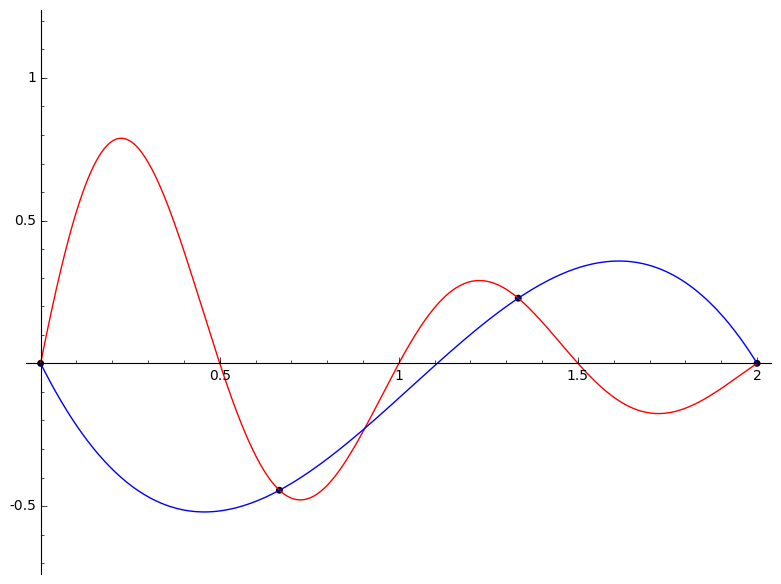
\includegraphics[scale=0.2]{figures/lagrange1}\quad
%    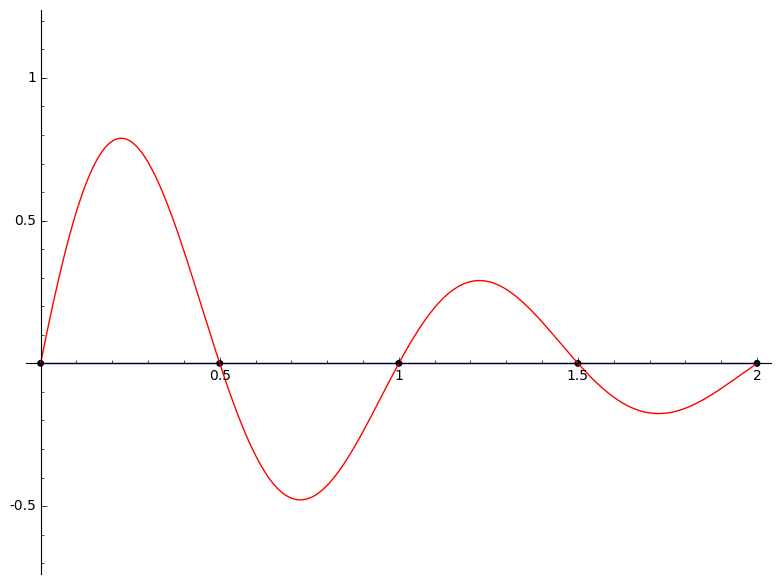
\includegraphics[scale=0.2]{figures/lagrange2}\quad
%    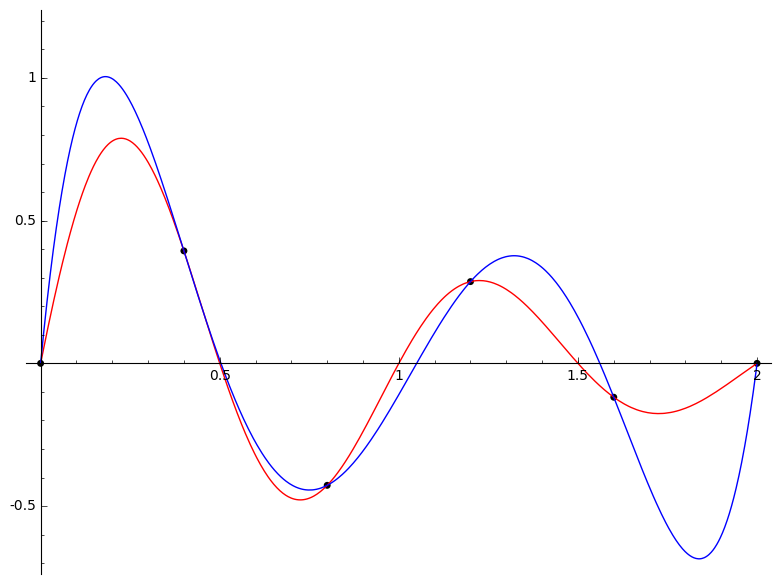
\includegraphics[scale=0.2]{figures/lagrange3}
%  \end{center}
%  \begin{center}
%    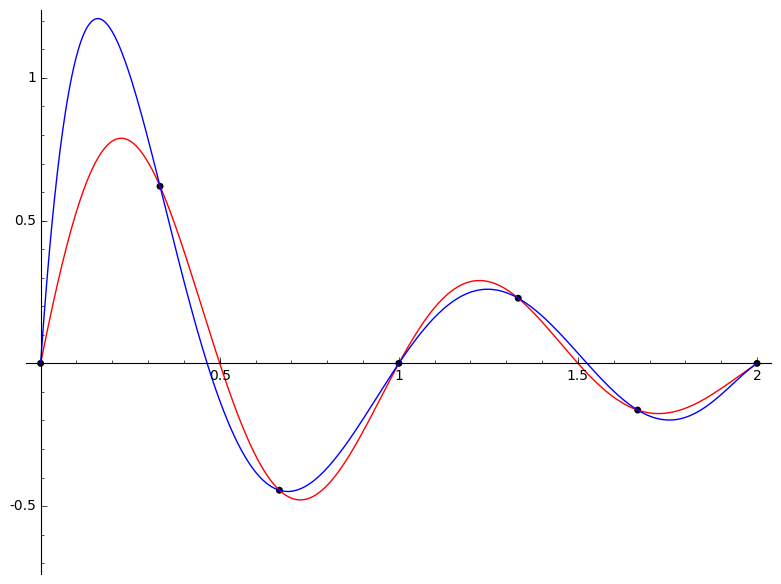
\includegraphics[scale=0.2]{figures/lagrange4}\quad
%    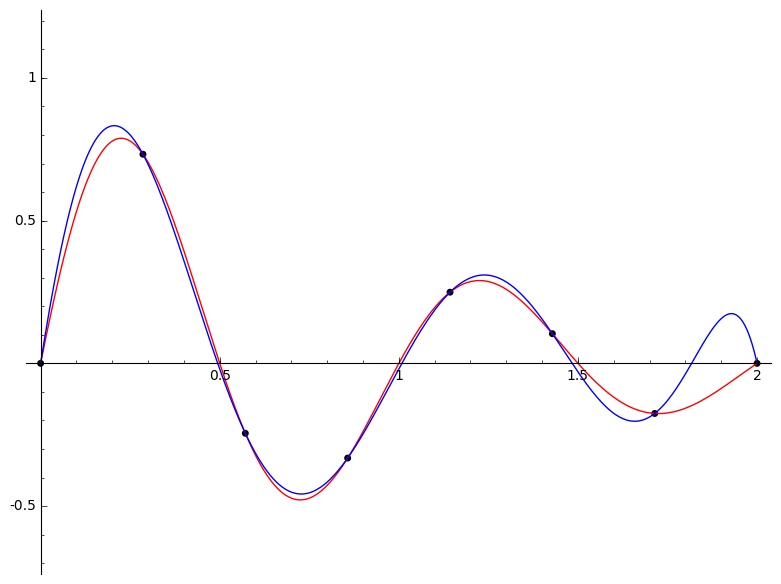
\includegraphics[scale=0.2]{figures/lagrange5}\quad
%    \includegraphics[scale=0.2]{figures/lagrange6}
%  \end{center}
%  
%  \item Voici l'interpolation de $f(x) = \frac{1}{1+8x^2}$
%  pour $n=7,10, 18$. La zone centrale de la courbe est bien interpolée mais autour de $-1$ et $+1$,
%  des <<bosses>>\ apparaissent. Ces bosses deviennent de plus en plus grandes en se décalant vers les extrémités. 
%  Il y a convergence simple mais pas convergence uniforme. Pour éviter ce phénomène, il faudrait mieux choisir les 
%  $x_i$.
%  \begin{center}
%    \includegraphics[scale=0.22]{figures/runge1}\quad
%    \includegraphics[scale=0.22]{figures/runge2}\quad
%    \includegraphics[scale=0.22]{figures/runge3}
%  \end{center} 
%  
%\end{enumerate}
%
%%%%%%%%%%%%%%%%%%%%%%%%%%%%%%%%%%%%%%%%%%%%%%%%%%%%%%%%%%%%%%%%%
%\section{\'Equations différentielles}
%
%
%%--------------------------------------------------------
%\subsection{\'Equations différentielles $y' = f(x,y)$}
%
%La commande \codeinline{desolve} permet de résoudre formellement des équations différentielles.
%Consultez la documentation, accessible par \codeinline{help(desolve)}.
%
%\begin{tp}
%\sauteligne
%\begin{enumerate}
%  \item 
%  \begin{enumerate}
%    \item Résoudre l'équation différentielle :
%  $$y' = y + x + 1.$$
%  Il s'agit donc de trouver toutes les fonctions $x\mapsto y(x)$ dérivables, telles que
%  $y'(x) = y(x) + x + 1$, pour tout $x\in \Rr$.
%    
%    \item Résoudre l'équation différentielle avec condition initiale :
%  $$y' = y + x + 1 \quad \text{ et } \quad y(0)=1.$$
%  \end{enumerate}
%  
%  
%
%  \item 
%  \begin{enumerate}
%    \item
%    Résoudre sur $\Rr_+^*$ l'équation différentielle :
%    $$x^2y' = (x-1)y.$$ 
%    \item Trouver la solution vérifiant $y(1)=2$.
%    
%    \item Peut-on trouver une solution sur $\Rr$ ?
%  \end{enumerate}
%    
%  \item Calculer la \defi{fonction logistique} $y(x)$, solution
%  de l'équation différentielle $$y'= y(1-y) - 1.$$       
%\end{enumerate}
%\end{tp}
%
%\begin{enumerate}
%  \item ~
%  
%  \insertcode{algos/equadiff-intro-tex1.sage}{equadiff-intro.sage (1)}
%  
%  \begin{enumerate}
%  \item 
%On commence par déclarer la variable $x$. 
%On définit une fonction $x \mapsto y(x)$ ainsi que sa dérivée $y'(x)$ 
%par \codeinline{diff(y,x)}. 
%On prendra ici la convention de noter $y'$ par \codeinline{yy}.
%L'équation différentielle $y' = y + x + 1$
%s'écrit donc \codeinline{yy == y+x+1}.
%On lance la résolution de l'équation différentielle par la fonction  
%\codeinline{desolve}, avec pour argument 
%l'équation différentielle à résoudre, ainsi que la fonction inconnue, qui est ici $y$. 
%\Sage\ renvoie :\\
%\centerline{\codeinline{-((x + 1)*e^(-x) - _C + e^(-x))*e^x}}
%\codeinline{_C} désigne une constante.
%Après simplification évidente, les solutions sont les :
%$$y(x) = -x-2 + C \exp(x) \quad \text{ où } \quad C \in \Rr.$$
%
%    \item Il est possible de préciser une condition 
%initiale grâce à l'argument optionnel \codeinline{ics} 
%(voir la dernière ligne du code ci-dessus), ici on 
%spécifie donc que l'on cherche la solution vérifiant $y(0)=1$.
%L'unique solution est alors : $y(x) = -x-2 + 3\exp(x)$, c'est-à-dire $C=3$.
%
%  \end{enumerate}
%
%  \item ~
%\insertcode{algos/equadiff-intro-tex2.sage}{equadiff-intro.sage (2)}
%
%  \begin{enumerate}
%    \item En se restreignant à $\Rr_+^*$ ($x>0$), on trouve $y(x) = Cx \exp(\frac1x)$, $C\in \Rr$.
%    
%    \item La solution vérifiant $y(1)=2$ est $y(x) = 2x \exp(\frac1x - 1)$,
%    c'est-à-dire $C = 2 \exp(-\frac1e)$.
%    
%    \item Sur $\Rr_-^*$ ($x<0$), les solutions sont aussi de la forme $y(x) = Cx \exp(\frac1x)$.
%
%    La seule solution définie sur $\Rr$ est donc la fonction nulle $y(x) = 0$ (et $C=0$). 
%    En effet si $C \neq 0$ il n'y a pas de limite finie en $0$.
%  \end{enumerate}
%  
%  \item ~ 
%  
%  \insertcode{algos/equadiff-intro-tex3.sage}{equadiff-intro.sage (3)}  
%  
%  \Sage\ ne résout pas directement cette équation différentielle. En effet, il renvoie une 
%  équation vérifiée par $y$ : 
%  \begin{equation}
%  \label{eq:diff1}
%  \frac{2}{3} \, \sqrt{3} \arctan\left(\frac{1}{3} \, \sqrt{3} {\big(2 \, y\left(x\right) - 1\big)}\right) = C + x.
%  \end{equation}
%  On demande alors à \Sage\ de résoudre cette équation, pour obtenir :
%  \begin{equation}
%  \label{eq:diff2}
%  y\left(x\right) = -\frac{\sqrt{3}}{2} \tan\left(\frac{\sqrt{3}}{2} C + \frac{\sqrt{3}}{2}  x\right) + \frac{1}{2}.
%  \end{equation}  
%  L'équation (\ref{eq:diff1}) a l'avantage d'être valide quel que soit $x$, alors 
%  que pour l'équation (\ref{eq:diff2}) il faudrait préciser l'intervalle de définition.
%  
%  
%
%\end{enumerate}
%
%
%%--------------------------------------------------------
%\subsection{Interprétation géométrique}
%
%
%\begin{itemize}
%  \item Les \defi{courbes intégrales} d'une équation différentielle $y' = f(x,y)$
%sont les graphes des solutions de cette équation.
%  
%  \item \`A chaque point d'une courbe intégrale, on associe un vecteur tangent.
%Si $y(x)$ est une solution de l'équation différentielle alors
%au point $(x,y(x))$ la tangente est portée par le vecteur $(x',y'(x))$.
%D'une part $x' = 1$ et d'autre part comme $y$ est solution de l'équation différentielle
%alors $y'(x) = f(x,y)$. Ainsi un \defi{vecteur tangent} en $(x,y)$ est $\big( 1 , f(x,y) \big)$.
%
%  \myfigure{1.3}{
%    \tikzinput{fig_formel_equadiff_vecteurs}\ \      
%  }
%  
%  \item %Gardons une équation différentielle $y' = f(x,y)$, dont nous ne connaissons pas les solutions.
%  Le \defi{champ de vecteurs} associé à l'équation différentielle
%$y' = f(x,y)$ est, en chaque point $(x,y)$ du plan, 
%le vecteur $\big( 1 , f(x,y) \big)$.
%
%  \item Voici ce qui signifie géométriquement \og résoudre \fg\ une équation différentielle.
%\`A partir d'un champ de vecteur, c'est-à-dire la donnée d'un vecteur
%attaché à chaque point du plan, il s'agit de trouver une courbe intégrale,
%c'est-à-dire une courbe qui en tout point est tangente aux vecteurs.
%
%
%  \item Comme on ne s'occupera pas de la norme des vecteurs, la donnée d'un champ de vecteur
%revient ici à associer à chaque point, la pente de la tangente au graphe 
%d'une solution passant par ce point.
%\end{itemize}
%
%\begin{tp}
%Nous allons étudier graphiquement l'équation différentielle 
%  $$y' = -xy.$$
%\begin{enumerate}
%  \item Représenter le champ de vecteurs associé à cette équation différentielle.
% 
%  \item 
%  \begin{enumerate}
%    \item Résoudre l'équation.
%    
%    \item Tracer, sur un même graphe, les courbes intégrales correspondant aux solutions
%    définies par $y(0)=k$, pour différentes valeurs de $k\in\Rr$.
%    
%    \item Que remarquez-vous ? Quel théorème cela met-il en évidence ? 
%  \end{enumerate}
%  
%  \item Tracer quelques isoclines de cette équation différentielle.
%\end{enumerate}
%\end{tp}
%
%Les \defi{isoclines} de l'équation différentielle $y' = f(x,y)$ sont les courbes sur lesquelles la tangente d'une courbe intégrale a 
%une pente donnée $c$, c'est-à-dire qu'une isocline est un ensemble
%$$\big\lbrace (x,y) \in \Rr^2 \mid f(x,y) = c \big\rbrace.$$
%\`A ne pas confondre avec les solutions ! En chaque point d'une isocline, 
%la solution passant par ce point croise cette isocline avec une pente $c$. 
%
%
%Voici quelques graphes :
%\begin{itemize}
%  \item Le champ de vecteurs (en rouge). 
%  \item Les courbes intégrales (en bleu).
%  \item Le champ de vecteurs superposé aux courbes intégrales : 
%  les vecteurs sont bien tangents aux courbes intégrales.
%
%  \item Les isoclines (en vert). Pour une isocline fixée, vérifier que chaque intersection 
%  avec les courbes intégrales se fait en des points où la tangente a toujours la même pente.
%\end{itemize}
%
%
%\begin{center}
% \includegraphics[scale=0.35]{figures/equadiff-courbe1.png} \qquad
%\includegraphics[scale=0.35]{figures/equadiff-courbe2.png} \\
%\includegraphics[scale=0.35]{figures/equadiff-courbe3.png} \qquad
%\includegraphics[scale=0.35]{figures/equadiff-courbe4.png} \\ 
%\end{center}
%
%
%\begin{enumerate}
%  \item Voici comment tracer le champ de vecteurs associé à $y' = f(x,y)$.
%  
%  \insertcode{algos/equadiff-courbe-tex1.sage}{equadiff-courbe.sage (1)}
%  
%  \begin{itemize}
%    \item Les variables de la fonction $f$ sont ici $u$ et $v$ pour ne pas interférer avec
%  la variable $x$ et la fonction $y$.
%  
%    \item N'hésitez pas à renormaliser les vecteurs $v$, (par exemple en $v/10$) pour plus de lisibilité. 
%  
%    \item  En fait la fonction \codeinline{plot_vector_field}, prédéfinie dans \Sage, trace aussi les champs de
%  vecteurs.
%  \end{itemize}
%
%  
% 
% 
%  
%  \item 
%  \begin{enumerate}
%    \item Les solutions de l'équation sont les
%    $$y(x) = C \exp\left(-\frac{x^2}{2}\right) \quad \text{ où } \quad C \in \R.$$
%    
%    \item Le code suivant résout l'équation différentielle et trace la solution 
%    avec la condition initiale $y(0)=k$, pour $k$ variant de \codeinline{ymin} à \codeinline{ymax}
%    avec un pas de \codeinline{delta}.
%    
%\insertcode{algos/equadiff-courbe-tex2.sage}{equadiff-courbe.sage (2)}
%    
%    \item Les courbes intégrales forment une partition 
%de l'espace : par un point il passe exactement une courbe intégrale. C'est 
%une conséquence du théorème d'existence et d'unicité de Cauchy-Lipschitz. 
%% Du point de vue de la physique, on pourrait dire que l'équation différentielle 
%% régit le comportement d'un système qui évolue de manière déterministe.
%
%  \end{enumerate}
%  \item Les isoclines sont définies par l'équation $f(x,y) = c$.
%  Elles se tracent par la commande \\
%  \centerline{\codeinline{implicit_plot(f-c, (x,xmin,xmax), (y,ymin, ymax))}}
%  
%  Ici les isoclines ont pour équation $-xy=c$, ce sont donc des hyperboles.
%  
%\end{enumerate}
%
%
%
%%--------------------------------------------------------
%\subsection{\'Equations différentielles du second ordre}
%
%\begin{tp}
%L'équation différentielle
%$$x''(t) +f x'(t)+ \frac{k}{m} x(t) = 0$$ 
%correspond au mouvement d'une masse $m$ 
%attachée à un ressort de constante $k>0$
%et des frottements $f\ge0$.
%
%  \myfigure{0.7}{
%    \tikzinput{fig_formel_equadiff_ressort}\ \      
%  }
%
%Résoudre et tracer les solutions pour 
%différentes valeurs de $f\ge0$ (prendre $k=1$, $m=1$), 
%avec les conditions initiales :
%$$x(0)= 1 \quad \text{ et } \quad x'(0)=0.$$
%\end{tp}
%
%Pour une valeur de $f$, l'équation se résout par : \\
%\centerline{\codeinline{desolve(diff(x,t,2) + f*diff(x,t) + k/m*x(t) == 0, x, ics=[0,1,0])}}
%
%Voici les solutions pour $f=0$, $f=1$, $f=2$ :
%
%\begin{center}
%\includegraphics[scale=0.25]{figures/equadiff-ressort1} \quad
%\includegraphics[scale=0.25]{figures/equadiff-ressort2} \quad
%\includegraphics[scale=0.25]{figures/equadiff-ressort3} 
%\end{center}
%
%
%\begin{itemize}
%  \item Cas $f=0$. Il n'y a pas de frottement. L'équation différentielle s'écrit
%  $x''+ \frac{k}{m} x = 0$. Pour $k=1$, $m=1$ alors l'équation est juste
%  $x''+ x = 0$ dont les solutions sont de la forme
%  $$x(t) = \lambda \cos t + \mu \sin t \qquad \lambda,\mu \in\Rr.$$
%  Avec les conditions initiales $x(0)=1$ et $x'(0)=0$, l'unique solution est 
%  $$x(t) = \cos t.$$
%  Il s'agit donc d'un mouvement périodique.
%  
%  \item Cas $0 < f < 2$. Les frottements sont faibles.
%  Par exemple pour $f=1$ la solution est 
%  $$\left(\frac{\sqrt{3}}{3} \sin\left(\frac{\sqrt{3}}{2} t\right) + 
%   \cos\left(\frac{\sqrt{3}}{2} t\right)\right)
%  e^{-\frac{1}{2} t}. $$
%  Il s'agit d'un mouvement amorti oscillant autour de la position d'origine $x=0$.
%  
%  \item Cas $f \ge 2$. Les frottements sont forts. 
%  Par exemple pour $f=2$ la solution est
%  $$x(t) = (t + 1)e^{-t}.$$
%  Il n'y a plus d'oscillations autour de la position d'origine.
%\end{itemize}
%


\auteurs{

\begin{itemize}
  \item Arnaud Bodin, Niels Borne, François Recher
  \item D'après un cours de calcul formel de Saïd Belmehdi, Jean-Paul Chehab, Bernard Germain-Bonne, François Recher donné à l'université Lille 1.
  \item Relu par Marc Mezzarobba et Paul Zimmermann.
\end{itemize}

}

\finchapitre
\end{document}

